\ChapterImageStar[cap:disenio]{Diseño de la solución}{./images/fondo.png}\label{cap:disenio}
\mbox{}\\

El presente capítulo tiene como objetivo fundamental traducir la decisión estratégica —la implementación de los universos Grid y Parallel— en un diseño técnico y estratégico concreto y ejecutable. Aquí se especifica la arquitectura de la solución, detallando los componentes de HTCondor que serán configurados o modificados, los flujos de trabajo establecidos para cada universo y los criterios de interoperabilidad con el universo Vanilla preexistente. Este diseño busca establecer las bases técnicas y metodológicas para la fase de implementación, propendiendo por la robustez, escalabilidad e integridad de la infraestructura de computación distribuida resultante. Además, busca ayudar al Grupo \GRID con el cumplimiento de sus objetivos estratégicos y el cierre de la brecha identificada en la caracterización.

\section{Definición de estrategia}
\noindent
La definición de la estrategia de diseño se fundamenta en una filosofía de desarrollo guiado por pruebas (\TDD), que es una disciplina de diseño y programación donde cada línea de código está escrita en respuesta a una prueba que el programador escribe justo antes de escribir el código \citep{4163024}. Antes de especificar los componentes arquitectónicos, se establece un conjunto de casos de prueba estructurados que definen de manera formal y verificable el comportamiento esperado de los universos Grid y Parallel. Estos casos, que funcionan como criterios de aceptación guiarán de manera iterativa el diseño de la solución, asegurando que cada decisión de implementación esté directamente alineada con la validación funcional del sistema.

Por último, se considera necesario establecer un nombre para el sistema. Esto con el fin de dar mayor claridad al lector y hacer más visibles los momentos en los que se habla del sistema resultado de este proyecto. Se opta por la \textit{Grid App} haciendo referencia al Grupo \GRID, que es el sujeto nuclear de este proyecto; al universo Grid, que es uno de los universos que se decidió implementar para este proyecto de aplicación después de la toma de decisiones estructurada mediante el análisis \DAR y el modelo computacional \textit{Grid} que es básicamente una infraestructura que provee gran capacidad computacional a un sistema distribuido haciendo uso de recursos geográficamente distribuidos \citep{8974490}.

\section{Casos de prueba}
\noindent

\subsection{Definición de requisitos}
\noindent
Para iniciar con la definición de casos de prueba, se establecen los requisitos que debe cumplir la \textit{Grid App} que están fundamentados en el análisis preliminar hecho anteriormente, principalmente en la descripción de la oportunidad para el Grupo \GRID.

\subsubsection{Requisitos funcionales}
\noindent
Según \cite{159342} un requisito funcional especifica una función que el sistema o que un componente del sistema es capaz de hacer. A continuación se definen los requisitos funcionales para la \textit{Grid App}.
\begin{table}[H]
	\centering
	\sffamily\scriptsize
	\setlength{\tabcolsep}{4pt}
	\renewcommand{\arraystretch}{1.3}
	\caption{Requisitos funcionales para \textit{Grid App}}
	\label{table:requisitosFuncionales}
	\begin{tabular}{|p{0.1\textwidth}|p{0.2\textwidth}|p{0.7\textwidth}|}
		\toprule
		\textbf{ID}                              & \textbf{Título}                               & \textbf{Descripción} \\
		\midrule
		RF1 & Soporte para Universos adicionales & El sistema debe permitir la ejecución de trabajos en al menos dos Universos adicionales a Vanilla (Grid y Parallel) \\
		\midrule
		RF2 & Orquestación de múltiples clústeres & El sistema debe permitir enviar trabajos hacia diferentes clústeres (Parallel, Vanilla) a través del Universo Grid. \\
		\midrule
		RF3 & Selección de destino & El sistema debe permitir que el usuario especifique el clúster de destino. \\
		\midrule
		RF4 & Monitoreo de trabajos & El sistema debe permitir el monitoreo de los trabajos enviados a los clústeres, mostrando su estado al usuario. \\
		\midrule
		RF5 & Ejecución MPI en Parallel & Un clúster debe soportar ejecución de trabajos basados en MPI en múltiples nodos (≥ N nodos configurados). \\
		\midrule
		RF6 & Redirección Grid-Parallel & El Grid Manager debe aceptar trabajos enviados al Universo Grid y, si la naturaleza del trabajo es paralelo, redirigirlos correctamente al Universo Parallel. \\
        \midrule
		RF7 & Redirección Grid-Vanilla & El Grid Manager debe aceptar trabajos enviados al Universo Grid y, si la naturaleza del trabajo es distribuido, redirigirlos correctamente al Universo Vanilla. \\
        \midrule
		RF8 & Registro centralizado de errores & El Grid Manager debe centralizar \textit{logs} de fallos de ejecución provenientes de cada clúster. \\
		\bottomrule
	\end{tabular}
\end{table}

\subsubsection{Requisitos no-funcionales}
\noindent
Según \cite{4384163} un requisito no-funcional es un atributo o una restricción de un sistema. A continuación se definen los requisitos no-funcionales para la \textit{Grid App}.
\begin{table}[H]
	\centering
	\sffamily\scriptsize
	\setlength{\tabcolsep}{4pt}
	\renewcommand{\arraystretch}{1.3}
	\caption{Requisitos no-funcionales para \textit{Grid App}}
	\label{table:requisitosNoFuncionales}
	\begin{tabular}{|p{0.1\textwidth}|p{0.2\textwidth}|p{0.7\textwidth}|}
		\toprule
		\textbf{ID}                              & \textbf{Título}                               & \textbf{Descripción} \\
		\midrule
		RNF1 & Transparencia de uso & El usuario no debe preocuparse por las configuraciones internas de cada clúster; el Grid Manager abstrae el destino mediante una interfaz más amigable. \\
		\midrule
		RNF2 & Usabilidad & La configuración de los nuevos Universos debe estar documentada y ser accesible mediante manual de despliegue para los usuarios del Grupo GRID. \\
		\midrule
		RNF3 & Disponibilidad & En caso de que un clúster esté inactivo, el Grid Manager debe registrar el error y permitir redirección a otro clúster disponible si el Universo es compatible. \\
		\bottomrule
	\end{tabular}
\end{table}

\subsection{Pruebas}
\noindent
Para esta sección, se definen las pruebas y los pasos para ejecutar cada prueba.
\begin{table}[H]
	\centering
	\renewcommand{\arraystretch}{1.2} % Espaciado reducido
	\fontsize{9pt}{10pt}\selectfont % Tamaño de fuente 8pt
	\begin{tabular}{|p{2cm}|p{4cm}|p{2.5cm}|p{4.7cm}|} % Total: 14cm
		\hline
		\textbf{ID del escenario de pruebas}    & ESC-01                                                                              & \textbf{ID de requisito}        & RF1, RF2, RF3, RF4, RF7, RF8, RNF1, RNF2, RNF3                      \\
		\textbf{Título de la prueba}            & Ejecución de trabajos en Universo Grid con repeticiones de iguales parámetros       & \textbf{Prerrequisitos}         & Grid Manager configurado con al menos un clúster soportando Vanilla \\
		\textbf{Descripción del caso de prueba} & Validar que el sistema soporta ejecución en Universo Grid hacia el Universo Vanilla & \textbf{Prioridad de la prueba} & Alta                                                                \\
		\hline
		\multicolumn{4}{|c|}{\textbf{Pasos de ejecución de las pruebas}}                                                                                                                                                                      \\
		\hline
		\textbf{ID de paso}                     & \textbf{Acción}                                                                     & \textbf{Datos de prueba}        & \textbf{Resultado esperado}                                         \\
		1                                       & Ingresar a la página                                                                & Link de la aplicación           & Página principal de la aplicación mostrada                          \\
		2                                       & Subir binario a través del selector de archivos                                     & Binario de ejecución            & Binario almacenado en el sistema de envío                           \\
		3                                       & Escribir argumentos adicionales (Opcional)                                          & Argumentos adicionales          & Argumentos seteados en el submit file dinámico                      \\
		4                                       & Seleccionar la naturaleza del trabajo (Distribuido)                                 & Naturalezas permitidas          & Universo seteado en el submit file dinámico                         \\
		5                                       & Seleccionar la información de distribución (Repeticiones con mismos parámetros)     & Distribuciones permitidas       & Agregada estructura necesaria al Submit file                        \\
		6                                       & Seleccionar cantidad de repeticiones                                                & Repeticiones necesarias         & Ciclo de envío en el archivo de shell creado                        \\
		7                                       & Seleccionar clúster más favorable                                                   & Métricas de clústeres           & Recurso remoto del grid en el submit file establecido               \\
		8                                       & Enviar trabajo                                                                      & Submit file generado            & Shell de envío y submit file ejecutado                              \\
		9                                       & Ver resultados a medida que van terminando                                          & Resultados de trabajos          & Salida de cada ejecución mostrada de forma organizada               \\
		\hline
	\end{tabular}
	\caption{Información ESC-01}
	\label{table:esc-01}
\end{table}

\begin{table}[H]
	\centering
	\renewcommand{\arraystretch}{1.2} % Espaciado reducido
	\fontsize{9pt}{10pt}\selectfont % Tamaño de fuente 8pt
	\begin{tabular}{|p{2cm}|p{4cm}|p{2.5cm}|p{4.7cm}|} % Total: 14cm
		\hline
		\textbf{ID del escenario de pruebas}    & ESC-02                                                                              & \textbf{ID de requisito}        & RF1, RF2, RF3, RF4, RF7, RF8, RNF1, RNF2, RNF3                      \\
		\textbf{Título de la prueba}            & Ejecución de trabajos en Universo Grid con variables parametrizables                & \textbf{Prerrequisitos}         & Grid Manager configurado con al menos un clúster soportando Vanilla \\
		\textbf{Descripción del caso de prueba} & Validar que el sistema soporta ejecución en Universo Grid hacia el Universo Vanilla & \textbf{Prioridad de la prueba} & Alta                                                                \\
		\hline
		\multicolumn{4}{|c|}{\textbf{Pasos de ejecución de las pruebas}}                                                                                                                                                                      \\
		\hline
		\textbf{ID de paso}                     & \textbf{Acción}                                                                     & \textbf{Datos de prueba}        & \textbf{Resultado esperado}                                         \\
		1                                       & Ingresar a la página                                                                & Link de la aplicación           & Página principal de la aplicación mostrada                          \\
		2                                       & Subir binario a través del selector de archivos                                     & Binario de ejecución            & Binario almacenado en el sistema de envío                           \\
		3                                       & Escribir argumentos adicionales (Opcional)                                          & Argumentos adicionales          & Argumentos seteados en el submit file dinámico                      \\
		4                                       & Seleccionar la naturaleza del trabajo (Distribuido)                                 & Naturalezas permitidas          & Universo seteado en el submit file dinámico                         \\
		5                                       & Seleccionar la información de distribución (Repeticiones con mismos parámetros)     & Distribuciones permitidas       & Agregada estructura necesaria al Submit file                        \\
		6                                       & Seleccionar variable parametrizable (De los argumentos adicionales)                 & Variables parametrizables       & Ciclo de envío en el archivo de shell creado                        \\
		7                                       & Establecer valor inicial                                                            & Valor inicial                   & Valor inicial del ciclo establecido                                 \\
		8                                       & Establecer valor final                                                              & Valor final                     & Valor final del ciclo establecido                                   \\
		9                                       & Establecer incremento                                                               & Incremento                      & Incremento del ciclo establecido                                    \\
		10                                      & Ver cantidad de repeticiones                                                        & Repeticiones necesarias         & Cantidad de repeticiones calculadas                                 \\
		11                                      & Seleccionar clúster más favorable                                                   & Métricas de clústeres           & Recurso remoto del grid en el submit file establecido               \\
		12                                      & Enviar trabajo                                                                      & Submit file generado            & Shell de envío y submit file ejecutado                              \\
		13                                      & Ver resultados a medida que van terminando                                          & Resultados de trabajos          & Salida de cada ejecución mostrada de forma organizada               \\
		\hline
	\end{tabular}
	\caption{Información ESC-02}
	\label{table:esc-02}
\end{table}

\begin{table}[H]
	\centering
	\renewcommand{\arraystretch}{1.2} % Espaciado reducido
	\fontsize{9pt}{10pt}\selectfont % Tamaño de fuente 9pt
	\begin{tabular}{|p{2cm}|p{4cm}|p{2.5cm}|p{4.7cm}|} % Total: 14cm
		\hline
		\textbf{ID del escenario de pruebas}    & ESC-03                                                        & \textbf{ID de requisito}        & RF1, RF2, RF3, RF4, RF5, RF6, RF8, RNF1, RNF2, RNF3                        \\
		\textbf{Título de la prueba}            & Ejecución de trabajos en Universo Parallel                    & \textbf{Prerrequisitos}         & Grid Manager configurado con al menos un clúster soportando Parallel       \\
		\textbf{Descripción del caso de prueba} & Validar que el sistema soporta ejecución en Universo Parallel & \textbf{Prioridad de la prueba} & Alta                                                                       \\
		\hline
		\multicolumn{4}{|c|}{\textbf{Pasos de ejecución de las pruebas}}                                                                                                                                                       \\
		\hline
		\textbf{ID de paso}                     & \textbf{Acción}                                               & \textbf{Datos de prueba}        & \textbf{Resultado esperado}                                                \\
		\hline
		1                                       & Ingresar a la página                                          & Link de la aplicación           & Página principal de la aplicación mostrada                                 \\
		2                                       & Subir binario a través del selector de archivos               & Binario de ejecución            & Binario almacenado en el sistema de envío                                  \\
		3                                       & Escribir argumentos adicionales (Opcional)                    & Argumentos adicionales          & Argumentos establecidos en el \textit{submit file} dinámico                \\
		4                                       & Seleccionar la naturaleza del trabajo (Paralelo)              & Naturalezas permitidas          & Universo establecido en el \textit{submit file} dinámico                   \\
		5                                       & Escribir cantidad de máquinas requeridas                      & Máquinas requeridas             & Parámetro ``\textit{machine\_count}'' del \textit{submit file} establecido \\
		6                                       & Escribir cantidad de núcleos solicitados por máquina          & Núcleos requeridos              & Parámetro ``\textit{required\_cpus}'' del \textit{submit file} establecido \\
		7                                       & Seleccionar clúster más favorable                             & Métricas de clústeres           & Recurso remoto establecido                                                 \\
		8                                       & Enviar trabajo                                                & \textit{Submit file} generado   & \textit{Script} de envío y \textit{submit file} ejecutado                  \\
		9                                       & Ver resultados a medida que van terminando                    & Resultados de trabajos          & Salida de cada ejecución mostrada de forma organizada                      \\
		\hline
	\end{tabular}
	\caption{Información ESC-03}
	\label{table:esc-03}
\end{table}


\subsection{Casos de uso}
\noindent
Luego de tener las pruebas que se van a ejecutar al sistema de la \textit{Grid App} ya definidas, se procede con la creación de un caso de uso por cada prueba. Esto tiene 3 motivaciones en este trabajo; (1) Mostrar la utilidad del sistema para un usuario ficticio, (2) Limitar el alcance del prototipo a unos casos de uso concretos y (3) Guiar el desarrollo hacia situaciones reales y la utilidad para los \textit{stakeholders}.

A continuación se definen los casos de uso:

\subsubsection{Caso 1: \textit{Montecarlo} para $\pi$}
\noindent
\begin{itemize}
    \item \textbf{Descripción:} En un laboratorio de investigación financiera, los analistas necesitan valuar instrumentos derivados complejos utilizando métodos \textit{Montecarlo} que requieren cientos de simulaciones. La infraestructura HTCondor distribuye estos cálculos estadísticos masivos a través de múltiples nodos, donde cada trabajo ejecuta una porción de las simulaciones para calcular aproximaciones de $\pi$ como prototipo, y luego consolida los resultados para obtener una mejor estimación que valide la confiabilidad del sistema en modelos de riesgo financiero.
    \item \textbf{Escenario de prueba relacionado:} ESC-01
\end{itemize}

\subsubsection{Caso 2: Conteo de números primos}
\noindent
\begin{itemize}
    \item \textbf{Descripción:} Un centro de criptografía debe analizar la distribución de números primos en intervalos grandes para evaluar la seguridad de algoritmos de encriptación RSA. HTCondor divide automáticamente estos rangos numéricos en sub intervalos que distribuye entre nodos heterogéneos, permitiendo el conteo concurrente de primos que demuestra la capacidad del sistema para manejar cargas computacionales intensivas.
    \item \textbf{Escenario de prueba relacionado:} ESC-02
\end{itemize}

\subsubsection{Caso 3: \textit{Quicksort} Paralelo}
\noindent
\begin{itemize}
    \item \textbf{Descripción:} Un instituto de genómica requiere ordenar cantidades enormes de datos de secuencias de ADN para identificar patrones de mutaciones genéticas. El algoritmo de \textit{quicksort} paralelo implementado con \MPI aprovechar los recursos agregados de memoria y procesamiento de múltiples máquinas bajo HTCondor, validando la capacidad de la infraestructura para coordinar trabajos que necesitan comunicación entre procesos (\IPC) en aplicaciones científicas.
    \item \textbf{Escenario de prueba relacionado:} ESC-03
\end{itemize}

\section{Modelado del sistema en Archimate}
\noindent
ArchiMate es un lenguaje de modelado estándar, abierto e independiente de~\textit{The Open Group} que permite representar de manera estructurada y general las diferentes capas de una arquitectura empresarial: negocio, aplicación y tecnología \citep{josey2016introduction}. Esto permite tener una visión integrada que facilita la comunicación entre los distintos actores de un negocio y que muestre cómo los procesos, los sistemas de información y la infraestructura tecnológica se relacionan entre sí.
A su vez, Archi es un Software que permite realizar diagramas de ArchiMate de forma sencilla y fue el Software elegido por el equipo de este proyecto para modelar las relaciones del proyecto con el negocio y varios elementos más. Archi permite dividir los modelos en vistas, que facilitan la organización y hacen más sencilla la labor de ampliar ciertos elementos o modelos importantes.

Cabe recalcar que algunos de los elementos como la misión y la visión no se muestran de forma completa en las vistas debido a su gran extensión textual. Sin embargo, con el fin de mostrar información completa, se mencionan y describen a continuación.

\begin{itemize}
    \item \textbf{Misión:} El Grupo de Investigación en Redes, Información y Distribución - GRID tiene como objetivo principal la realización de proyectos de investigación en temas relacionados principalmente con soluciones informáticas en Infraestructura Computacional, la Ingeniería de Software, el Análisis de Datos y la Informática Educativa. Hacer investigación en los temas mencionados, así como realizar proyectos interdisciplinarios deberá redundar en conocimientos frescos y la adopción de nuevas tecnologías que contribuyan al desarrollo académico del Programa Ingeniería de Sistemas y Computación, la Maestría en Ingeniería, y la Maestría y el Doctorado en Educación de la Universidad del Quindío. Luego de 10 años de existencia, de haber superado exitosamente los procesos de formación a nivel doctoral y de maestría de nuestros integrantes y de haber logrado la categoría C en el escalafón nacional de Ministerio de Ciencia, Tecnología e Innovación, nuestros esfuerzos estarán centrados en: (1) la formación de estudiantes a nivel de pregrado, maestría y doctorado; (2) fortalecer los lazos de amistad y colaboración con investigadores y grupos de investigación a nivel nacional e internacional; (3) la realización de proyectos de investigación y desarrollo de productos de nuevo conocimiento que busquen dar solución a problemas de la sociedad; y (4) aumentar la visibilidad del grupo y mejorar la categoría en el escalafón de MinCiencias.
    \item \textbf{Visión:} Para el año 2025, el Grupo de Investigación en Redes, Información y Distribución - GRID de la Facultad de Ingeniería de la Universidad del Quindío será un grupo consolidado y reconocido en la más alta categoría del escalafón nacional del Ministerio de Ciencia Tecnología e Innovación, que a través de sus aportes sea tenido en cuenta en la toma de decisiones a nivel regional y nacional; y con reconocimiento internacional mediante la realización de trabajos en colaboración con investigadores de otras universidades nacionales y extranjeras. Misión: Somos un grupo de profesores universitarios dedicados a realizar investigación en áreas tecnológicas orientadas a facilitar procesos y resolver problemas de la comunidad académica, de la sociedad que nos rodea y del sector productivo, mediante la adaptación de tecnologías o el desarrollo de soluciones informáticas en Infraestructura Computacional, la Ingeniería de Software, el Análisis de Datos y la Informática Educativa que constituyan un aporte al desarrollo social, económico y tecnológico de la región y el país.
    \item \textbf{Objetivo estratégico 1:} Realizar proyectos de investigación en los temas relacionados con las áreas de interés del grupo, así como proyectos interdisciplinarios que permitan la adopción de conocimientos y nuevas tecnologías que contribuyan al desarrollo de la región, del país y de la comunidad académica mundial.
    \item \textbf{Objetivo estratégico 2:} Establecer contactos con otros grupos de investigación interesados en temáticas similares, pertenecientes a otras instituciones de educación superior, tanto a nivel nacional como internacional.
    \item \textbf{Objetivo estratégico 3:} Impulsar la investigación dentro de la Universidad del Quindío y la Facultad de Ingeniería, particularmente en el programa Ingeniería de Sistemas y Computación, el programa de Maestría en Ingeniería, y los programas de Maestría y Doctorado en Educación.
    \item \textbf{Objetivo estratégico 4:} Establecer una comunidad académica con la participación de estudiantes de pregrado y posgrado, profesores y jóvenes investigadores.
\end{itemize}

\subsection{Vista de misión, visión y objetivos}
\noindent
        En la Figura \ref{fig:archiMVOView} se muestra las relaciones entre la misión, la visión y los objetivos estratégicos del negocio. Además, se muestran los ámbitos clave en los que se enfoca el negocio para cumplir con sus objetivos estratégicos. Esta última información se tomó de conversaciones informales con el representante del negocio para este proyecto, quien manifestó que estos son los enfoques que se le debe dar al proyecto y están dados por la organización a la que está adscrito el negocio, que para nuestro caso específico es el Grupo \GRID.\begin{figure}[H]
	\centering
	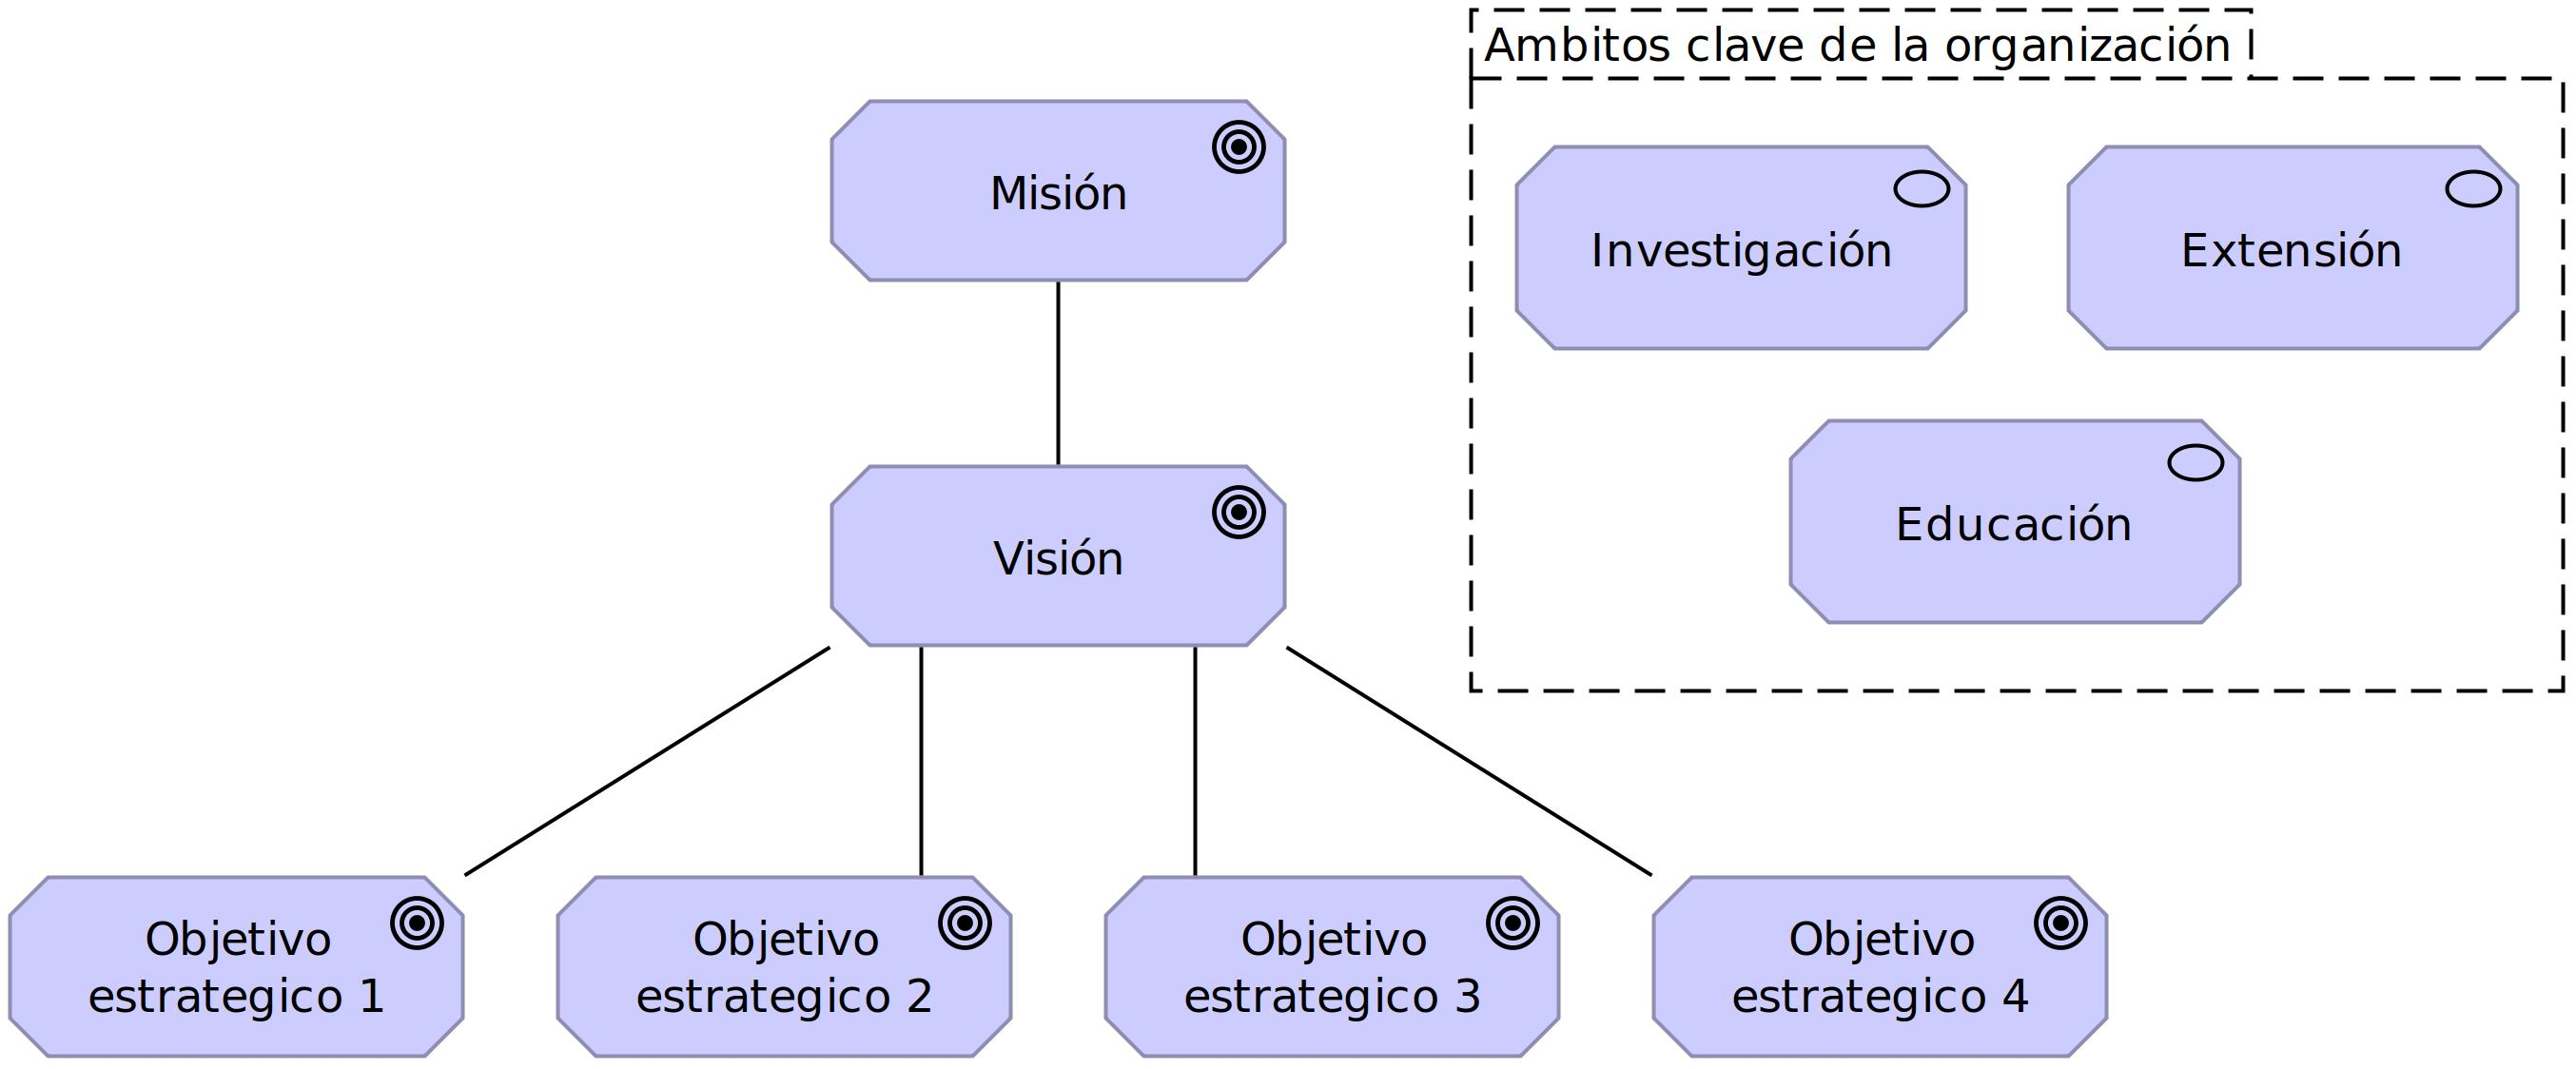
\includegraphics[scale=0.15]{tablas-images/archi/Mission-Values-Vision View.jpg}
	\caption{Vista de misión, visión y objetivos}
    \label{fig:archiMVOView}
\end{figure}

\subsection{Vista de mapa de valor estratégico}
\noindent
En la Figura \ref{fig:archiSVMView} se muestra el valor estratégico del negocio desde distintas perspectivas y su descomposición hacia otros valores más concretos. Todo esto con el fin de conocer que perspectivas son de más interés para el negocio y cuáles valores componen dichas perspectivas. Esto ocurre en capa de motivación, por lo que estos valores estratégicos identificados servirán como los principios orientadores de la estrategia del negocio.

\begin{figure}[H]
	\centering
	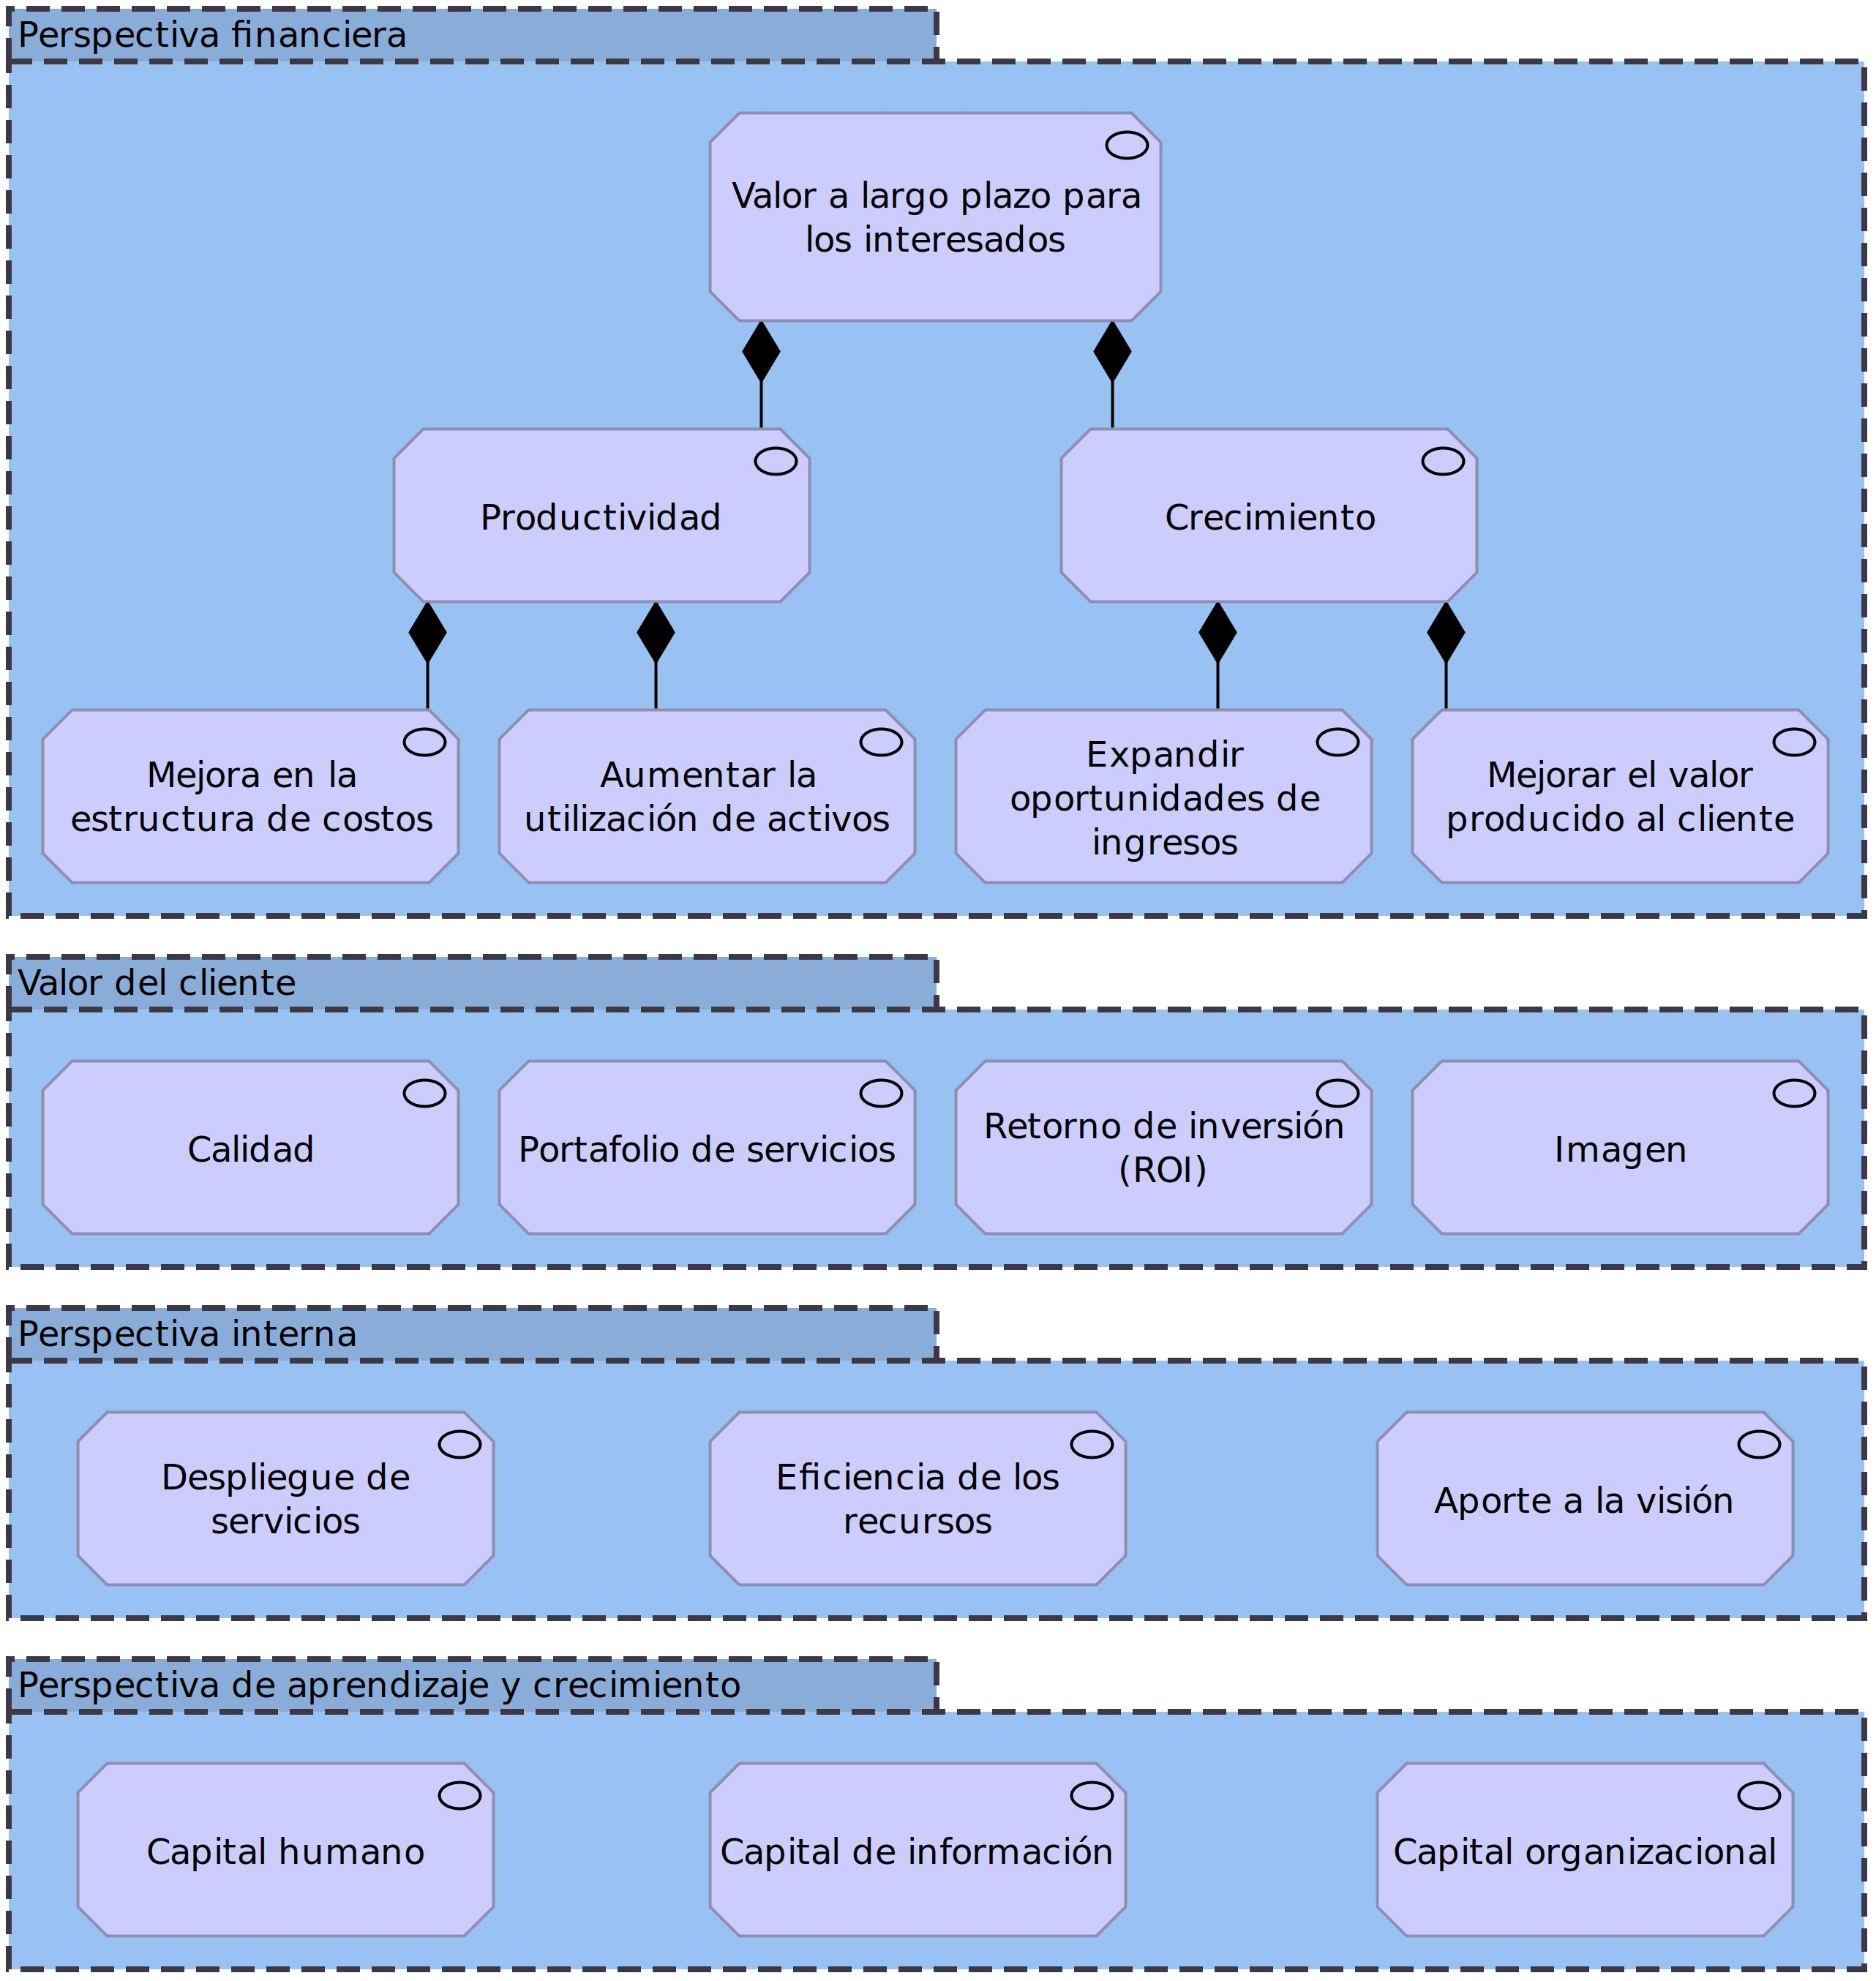
\includegraphics[scale=0.15]{tablas-images/archi/Strategic Value Map View.jpg}
	\caption{Vista de mapa de valor estratégico}
    \label{fig:archiSVMView}
\end{figure}

\subsection{Vista de objetivos}
\noindent
En la Figura \ref{fig:archiGoalsView} se muestra un desglose completo de los objetivos del negocio. Para este fin se usó una variación de una estrategia conocida como 5W, que usa cinco preguntas para obtener información completa sobre un elemento. Estas preguntas son: ¿Quién?, ¿Qué?, ¿Cuándo?, ¿Dónde? Y ¿Por qué? \citep{5WAmitava}. Para el desglose de los objetivos del negocio en esta vista del modelo se hizo necesarias solo cuatro preguntas como se muestra en la Figura \ref{fig:archiGoalsView}. Así, podemos ver como está compuesta la motivación del negocio y los elementos que están en torno a los objetivos estratégicos.

\begin{figure}[H]
	\centering
	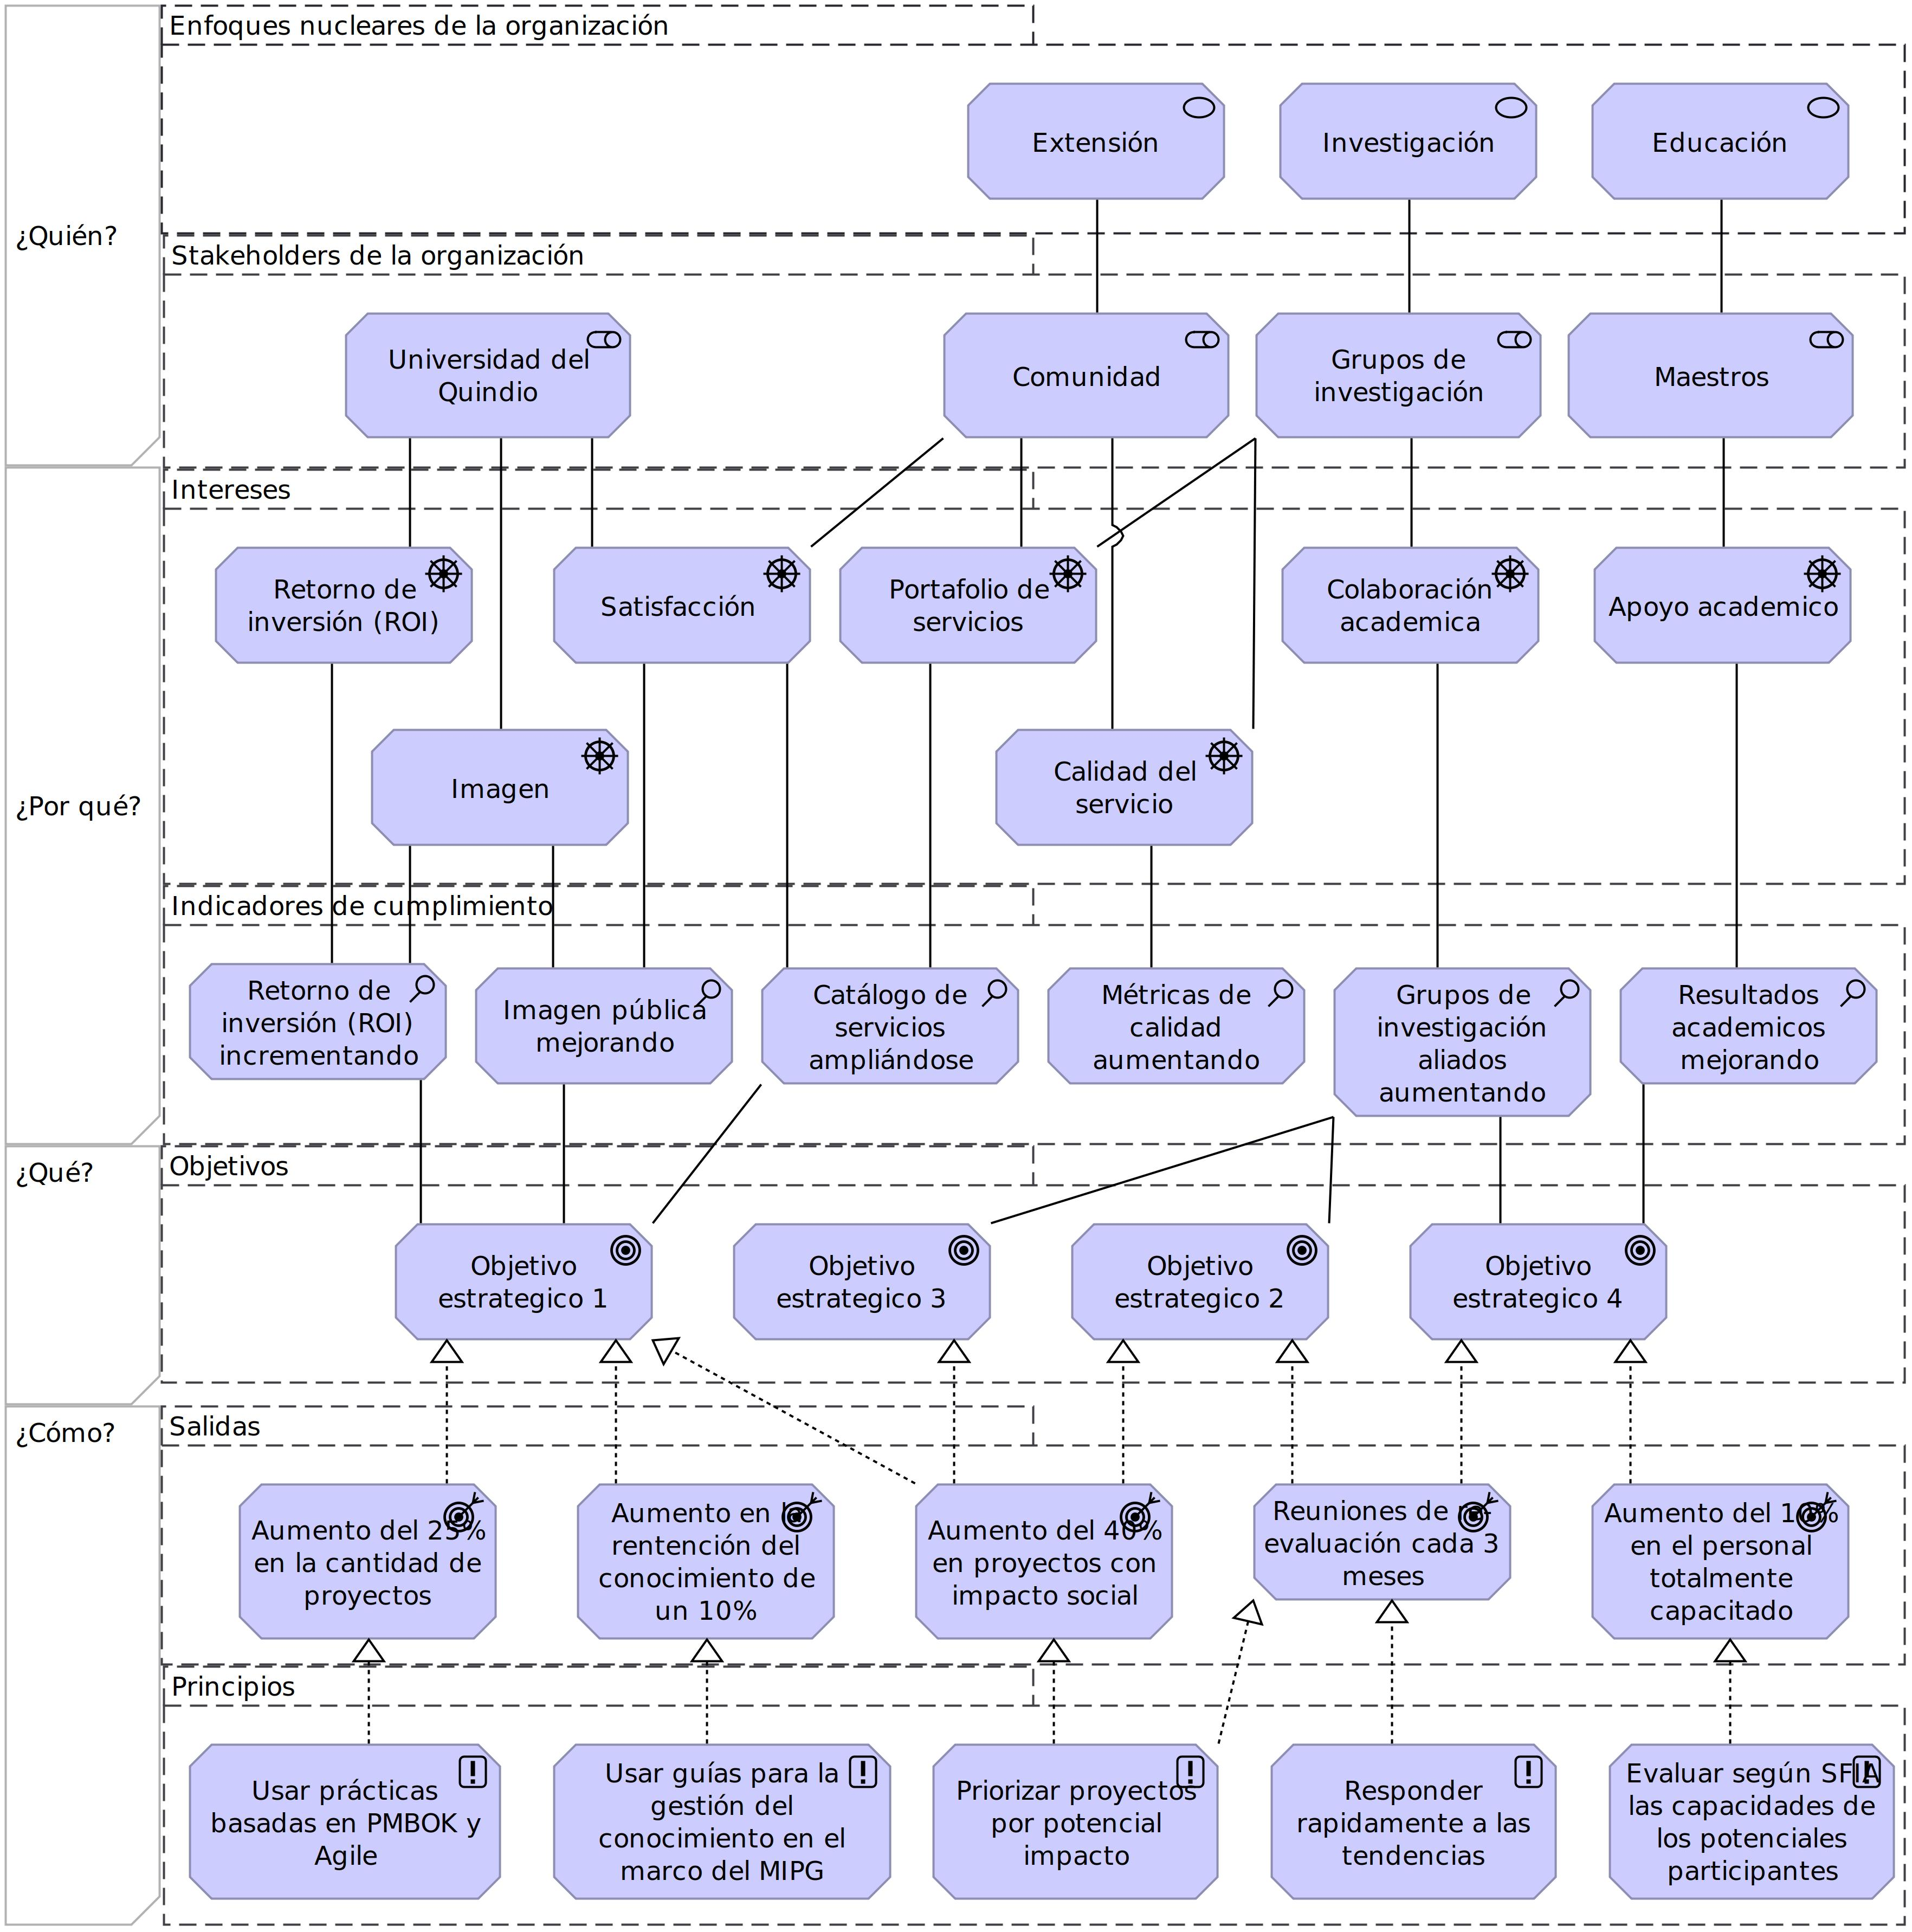
\includegraphics[scale=0.12]{tablas-images/archi/Goals View.jpg}
	\caption{Vista de objetivos}
    \label{fig:archiGoalsView}
\end{figure}

\subsection{Vista de servicio de negocio}
\noindent
En la Figura \ref{fig:archiBSView} se muestra la estructura del servicio de negocio que el proyecto relatado en este documento buscar intervenir, desde los objetivos estratégicos en cuanto a motivación hasta los componentes de aplicación, pasando por los servicios de aplicación y el servicio de negocio con una estructura mínima. Cabe recalcar que los nombres en inglés de algunos componentes corresponden a nombres propios que se le asignaron al componente

\begin{figure}[H]
	\centering
	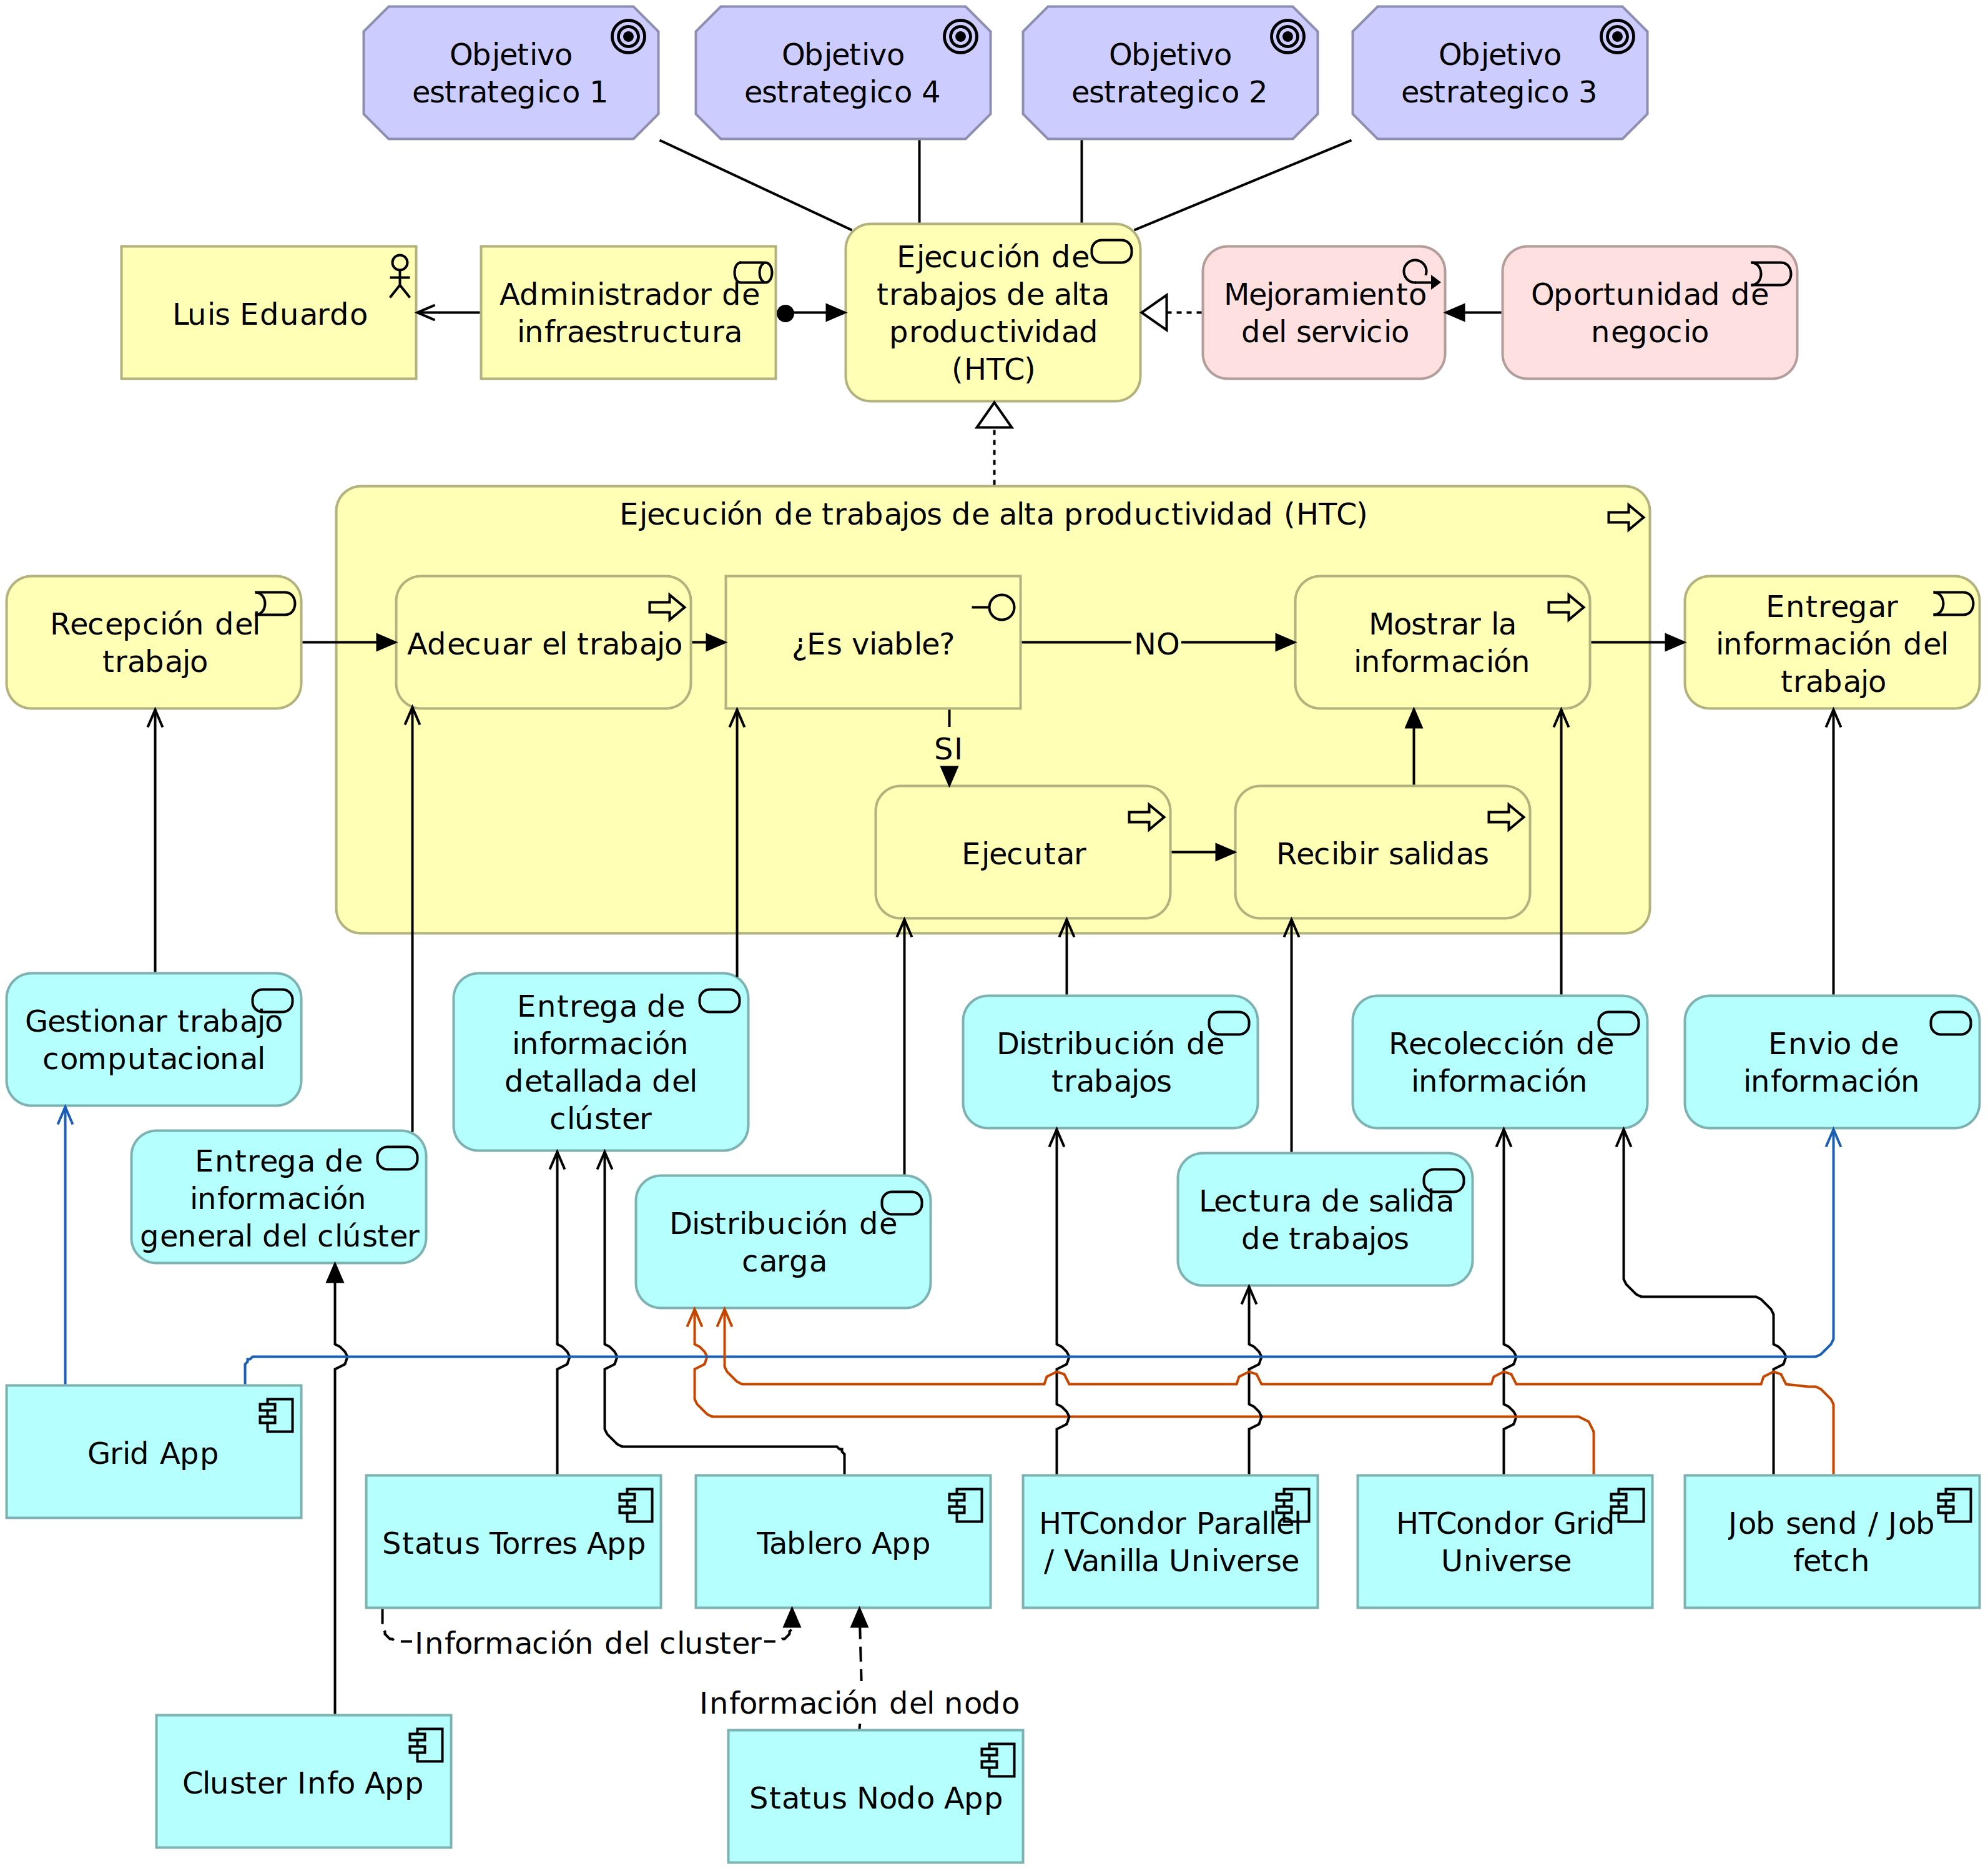
\includegraphics[scale=0.13]{tablas-images/archi/Business Service View.jpg}
	\caption{Vista de servicio de negocio}
    \label{fig:archiBSView}
\end{figure}

\subsection{Vista de aplicación}
\noindent
En la Figura \ref{fig:archiAppView} se muestran de forma general, las características y procesos de las aplicaciones que componen la solución, además de la comunicación entre dichas aplicaciones y la información de intercambio. Sin embargo, la vista que nos ofrece ArchiMate en capa de aplicación puede ser un poco limitada cuando el objetivo es describir a detalle la forma en que funciona cada componente de la aplicación y del sistema en general. Por lo que se decide complementar este modelo con otros diagramas usando otros lenguajes de modelado un poco más adelante.

\begin{figure}[H]
	\centering
	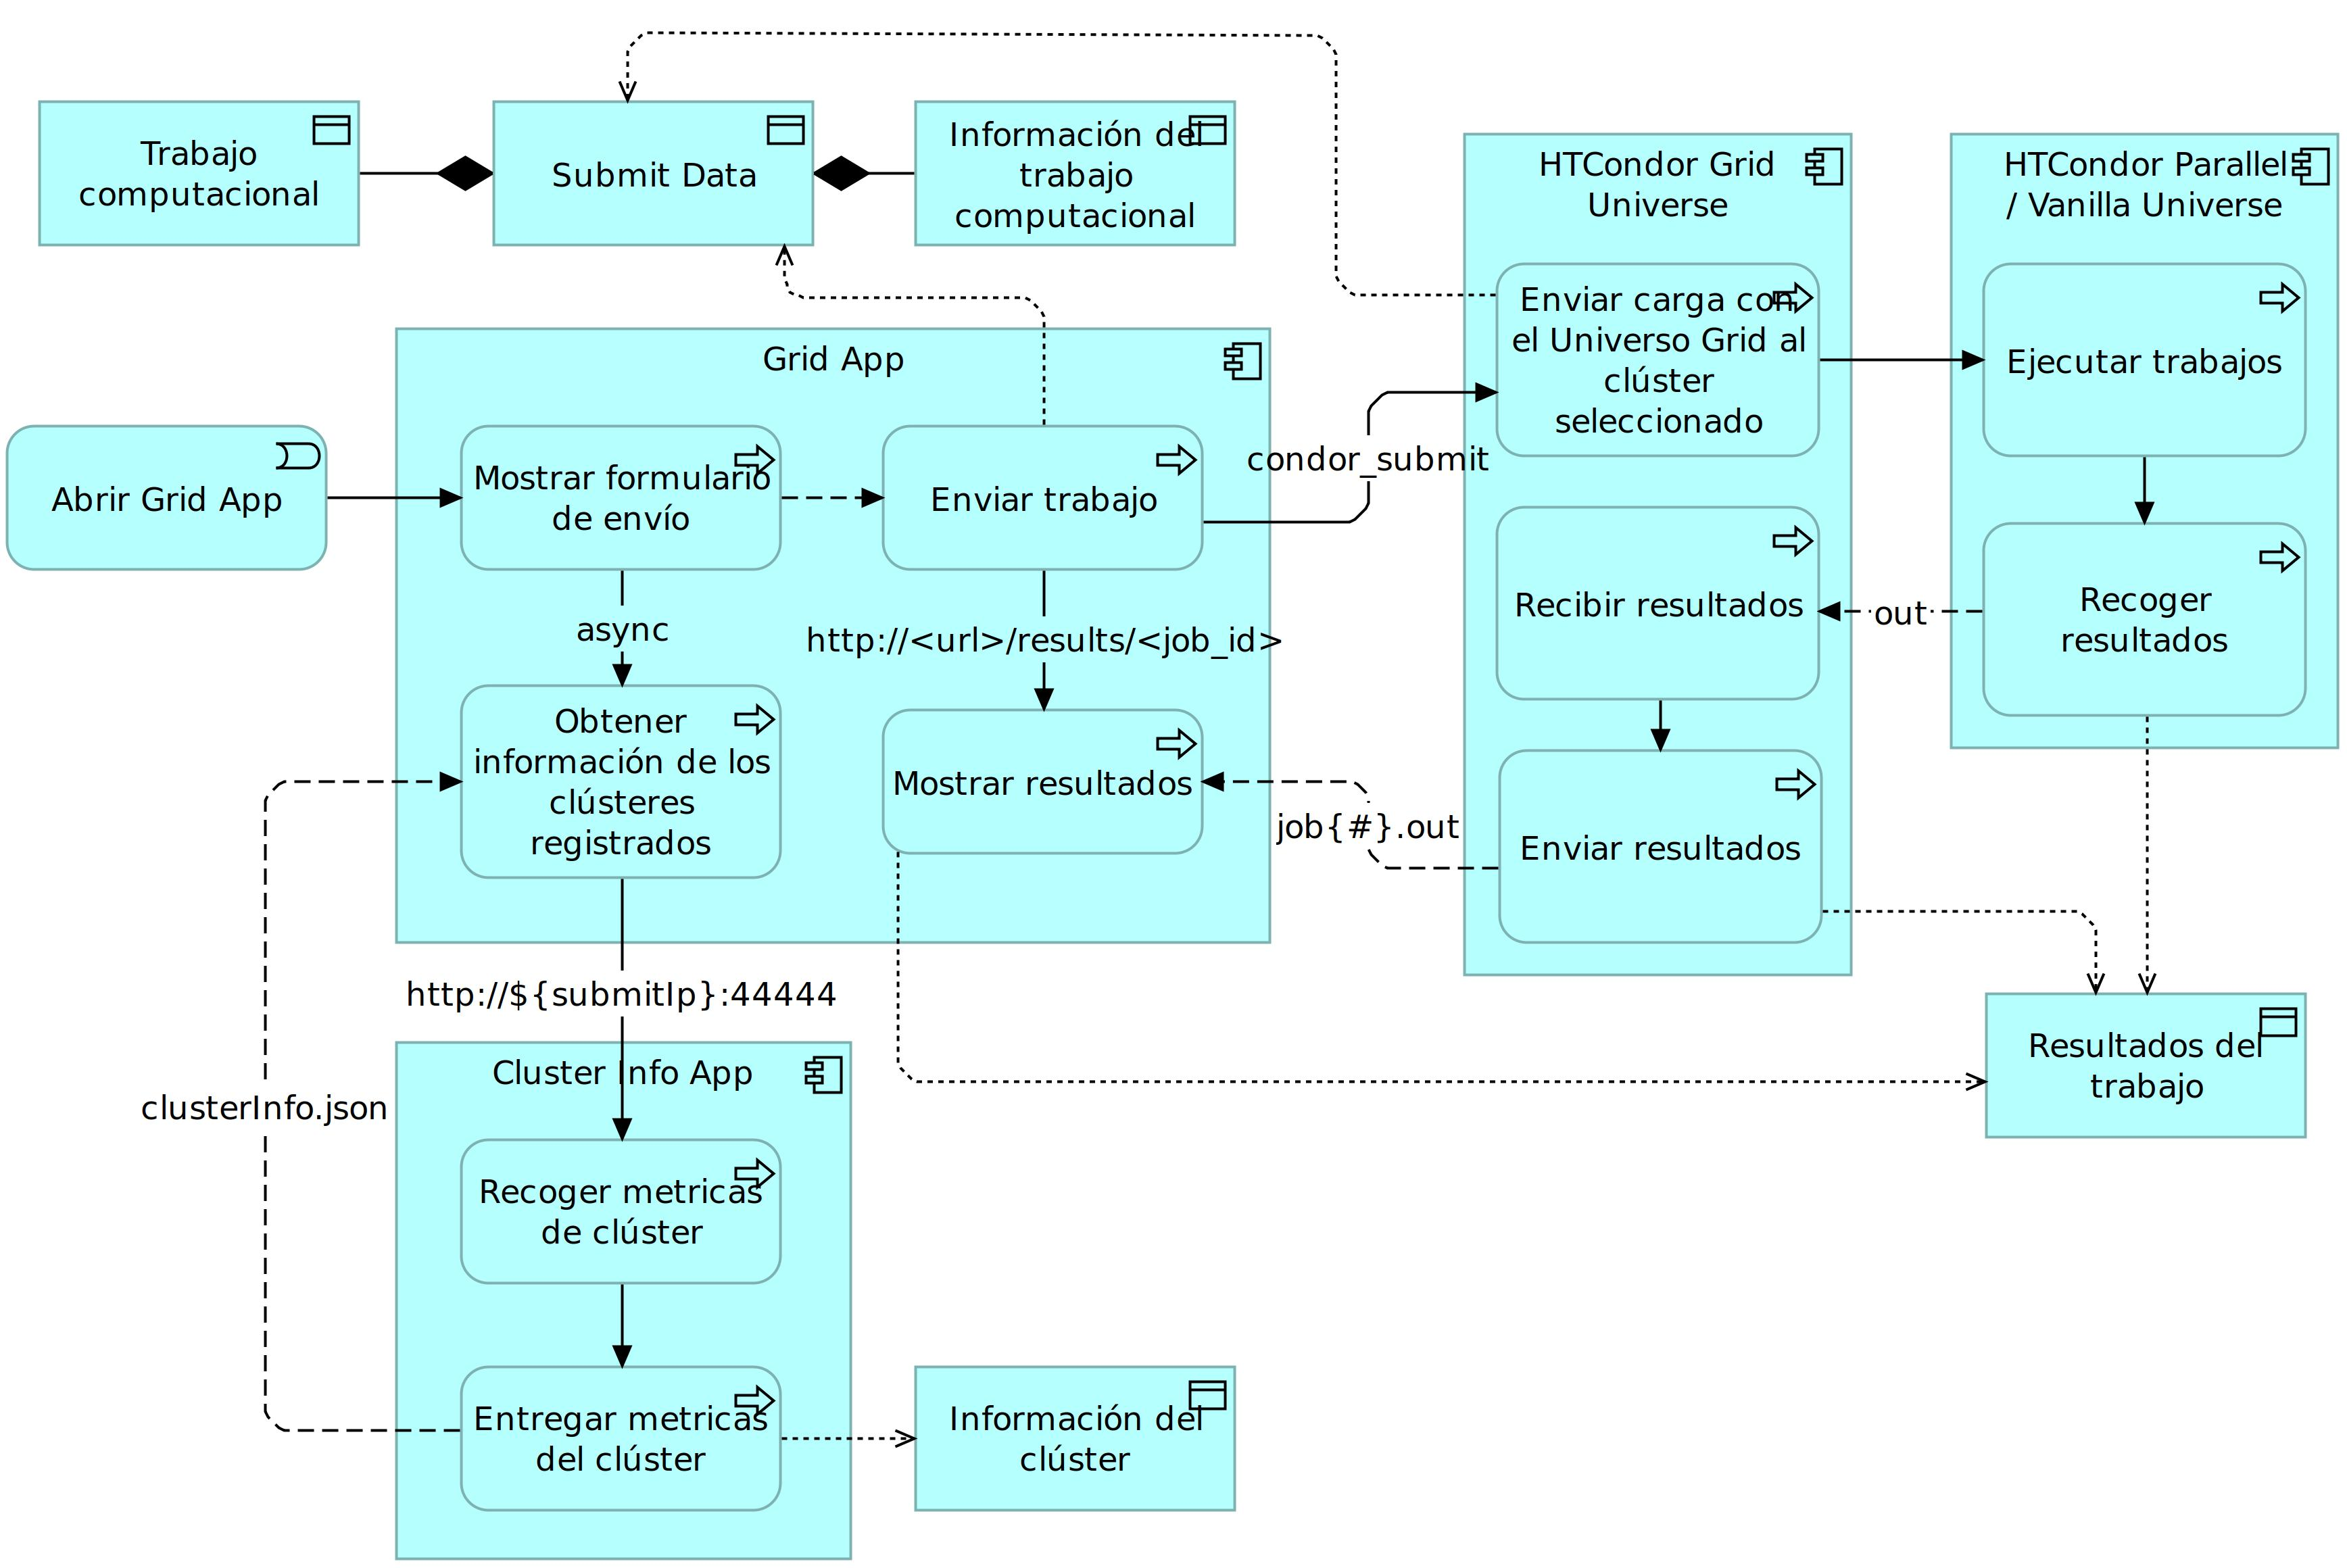
\includegraphics[scale=0.12]{tablas-images/archi/Application View.jpg}
	\caption{Vista de aplicación}
    \label{fig:archiAppView}
\end{figure}

\subsection{Vista de infraestructura}
\noindent
En la Figura \ref{fig:archiInfrastructureView} se muestran de forma general, las características de los nodos de la infraestructura que componen la solución, además de las relaciones entre dichos nodos y su relación con las aplicaciones que corren en ellos. Sin embargo, al igual que pasa en la capa de aplicación, la vista que nos ofrece ArchiMate en capa de infraestructura puede ser un poco limitada cuando el objetivo es describir a detalle la forma en que funciona cada nodo de la infraestructura y su comunicación física. Por lo que se decide complementar este modelo con otros diagramas usando otros lenguajes de modelado un poco más adelante.

\begin{figure}[H]
	\centering
	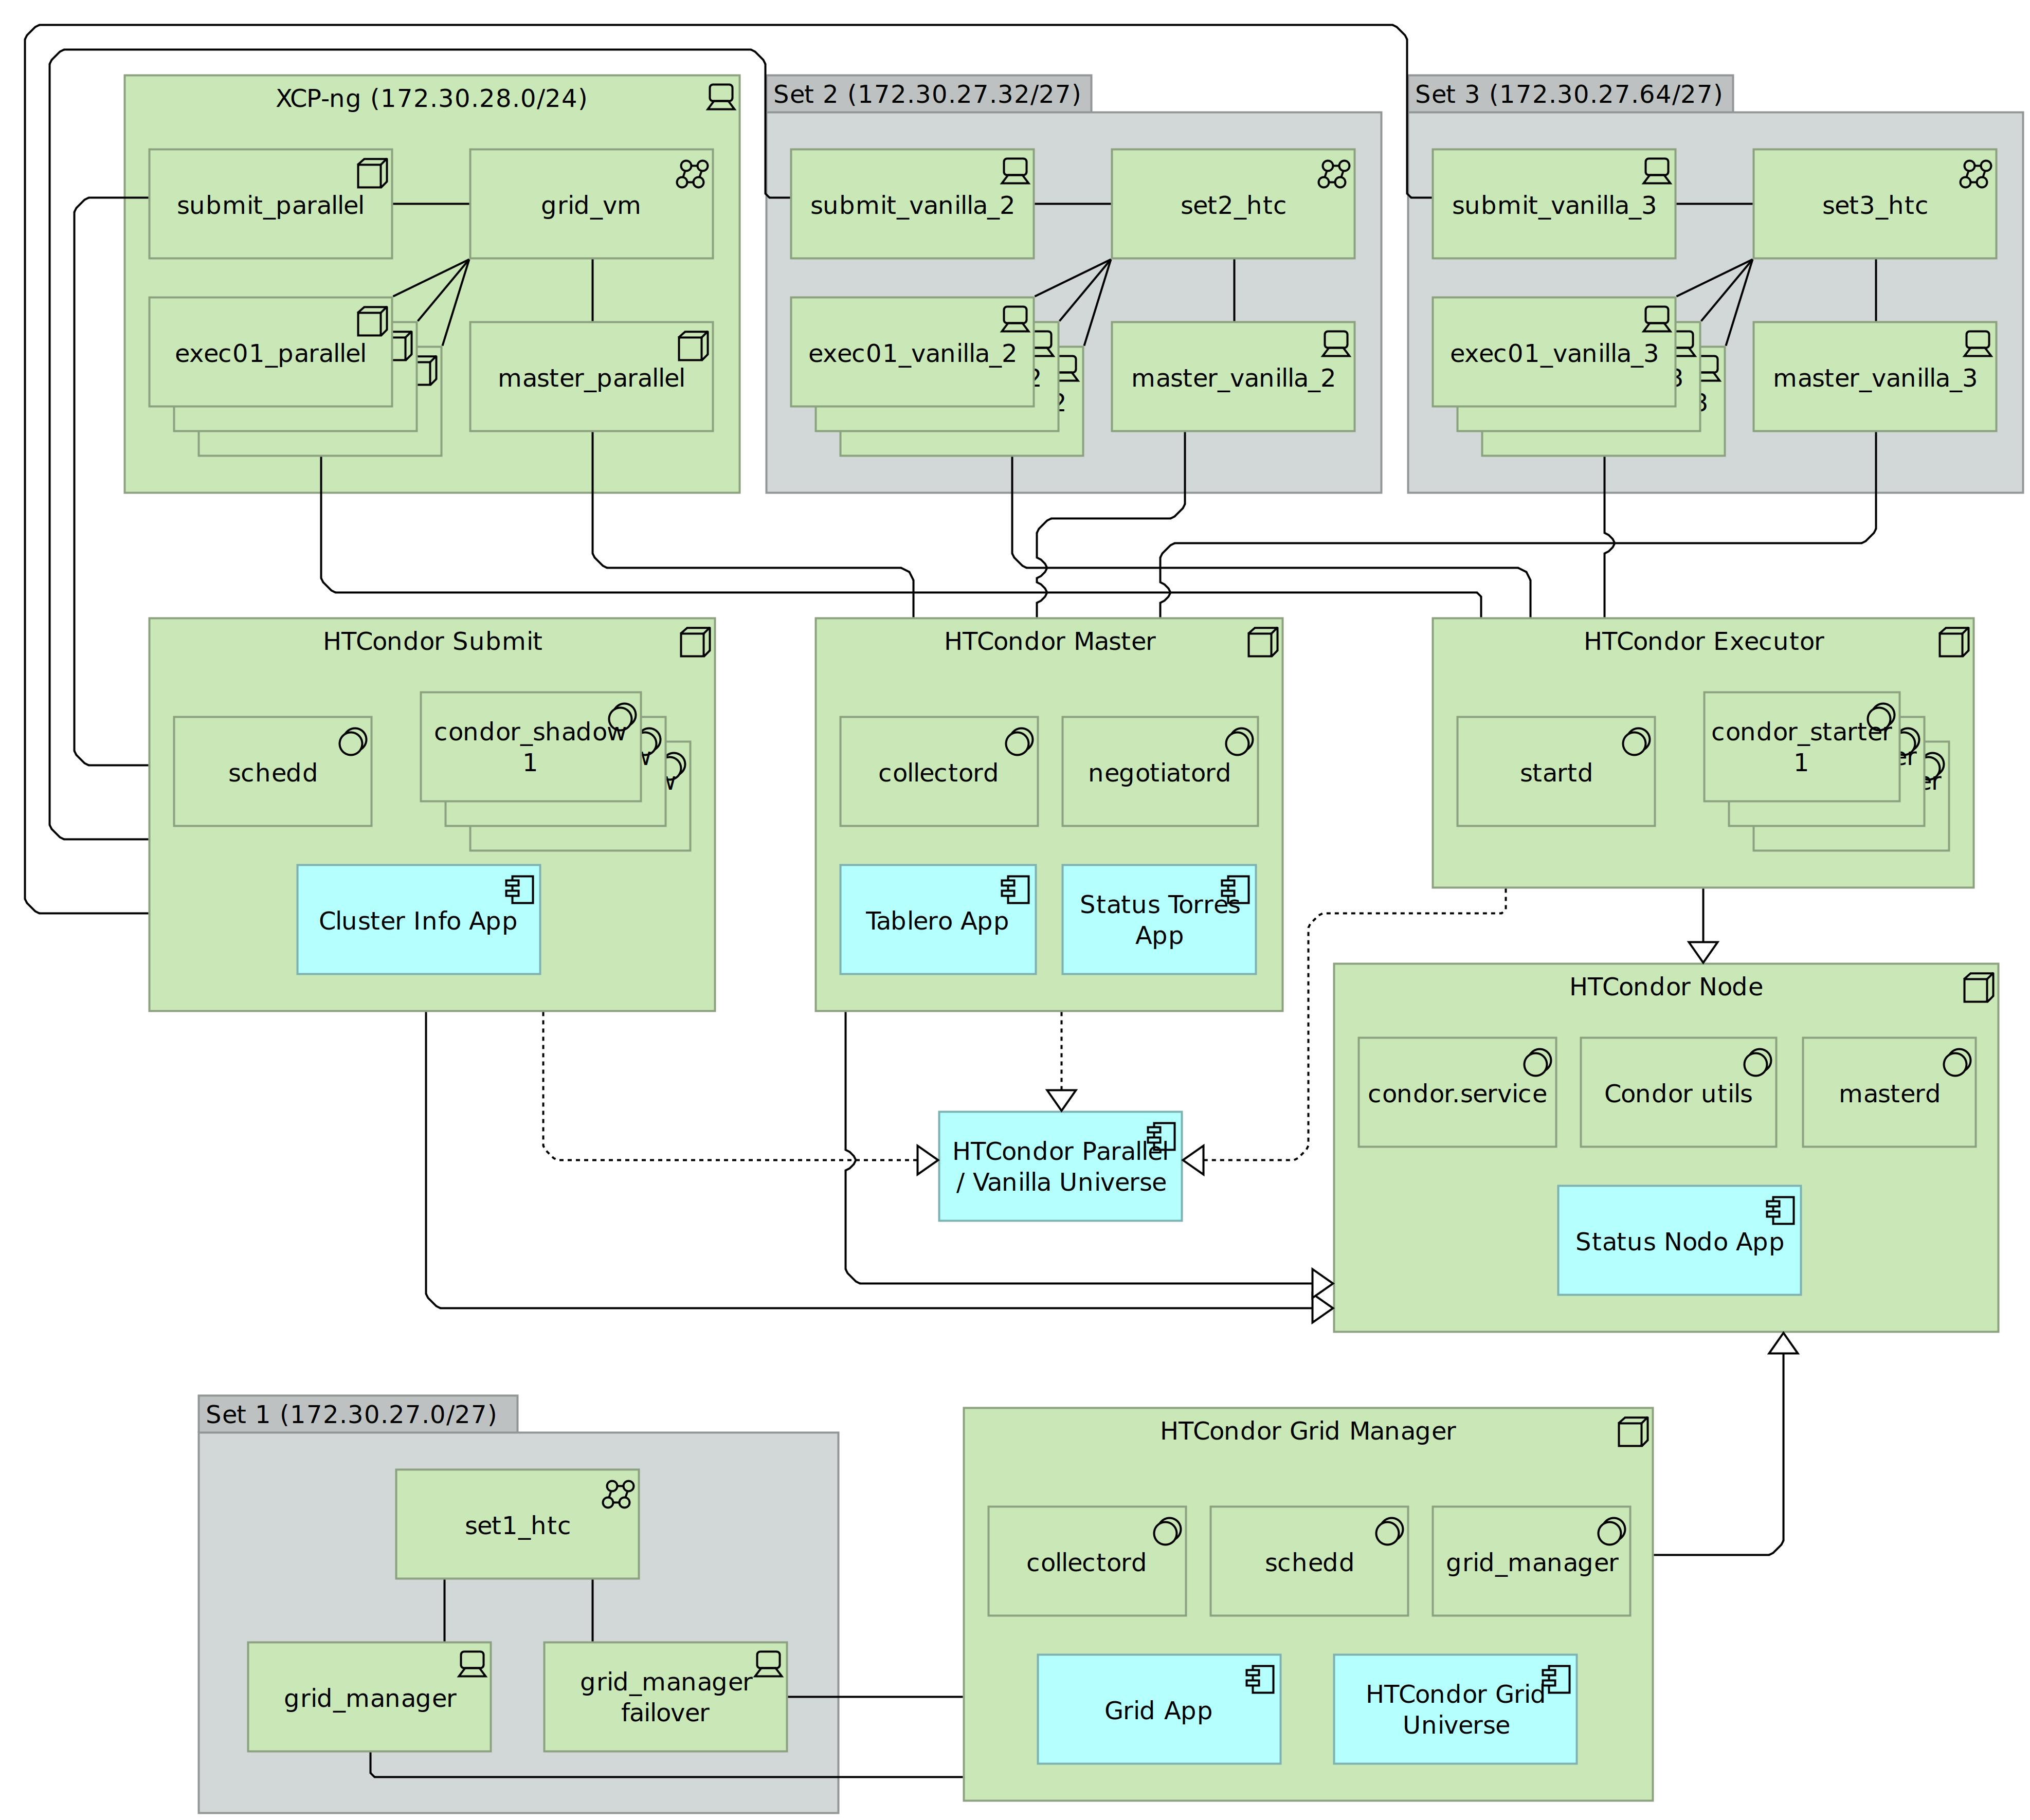
\includegraphics[scale=0.103]{tablas-images/archi/Infrastructure View.jpg}
	\caption{Vista de infraestructura}
    \label{fig:archiInfrastructureView}
\end{figure}

\subsection{Vista por capas}
\noindent
El último modelo de ArchiMate que compone la solución es el mostrado en la Figura \ref{fig:archiLayeredView} en donde se unen de forma general los demás modelos mostrados anteriormente y se muestran sus relaciones a alto nivel. Todo esto con el fin de dar una visión general de las capas que componen la solución y así tener una idea global de la forma en que cada componente se comunica con los demás.

\begin{figure}[H]
	\centering
	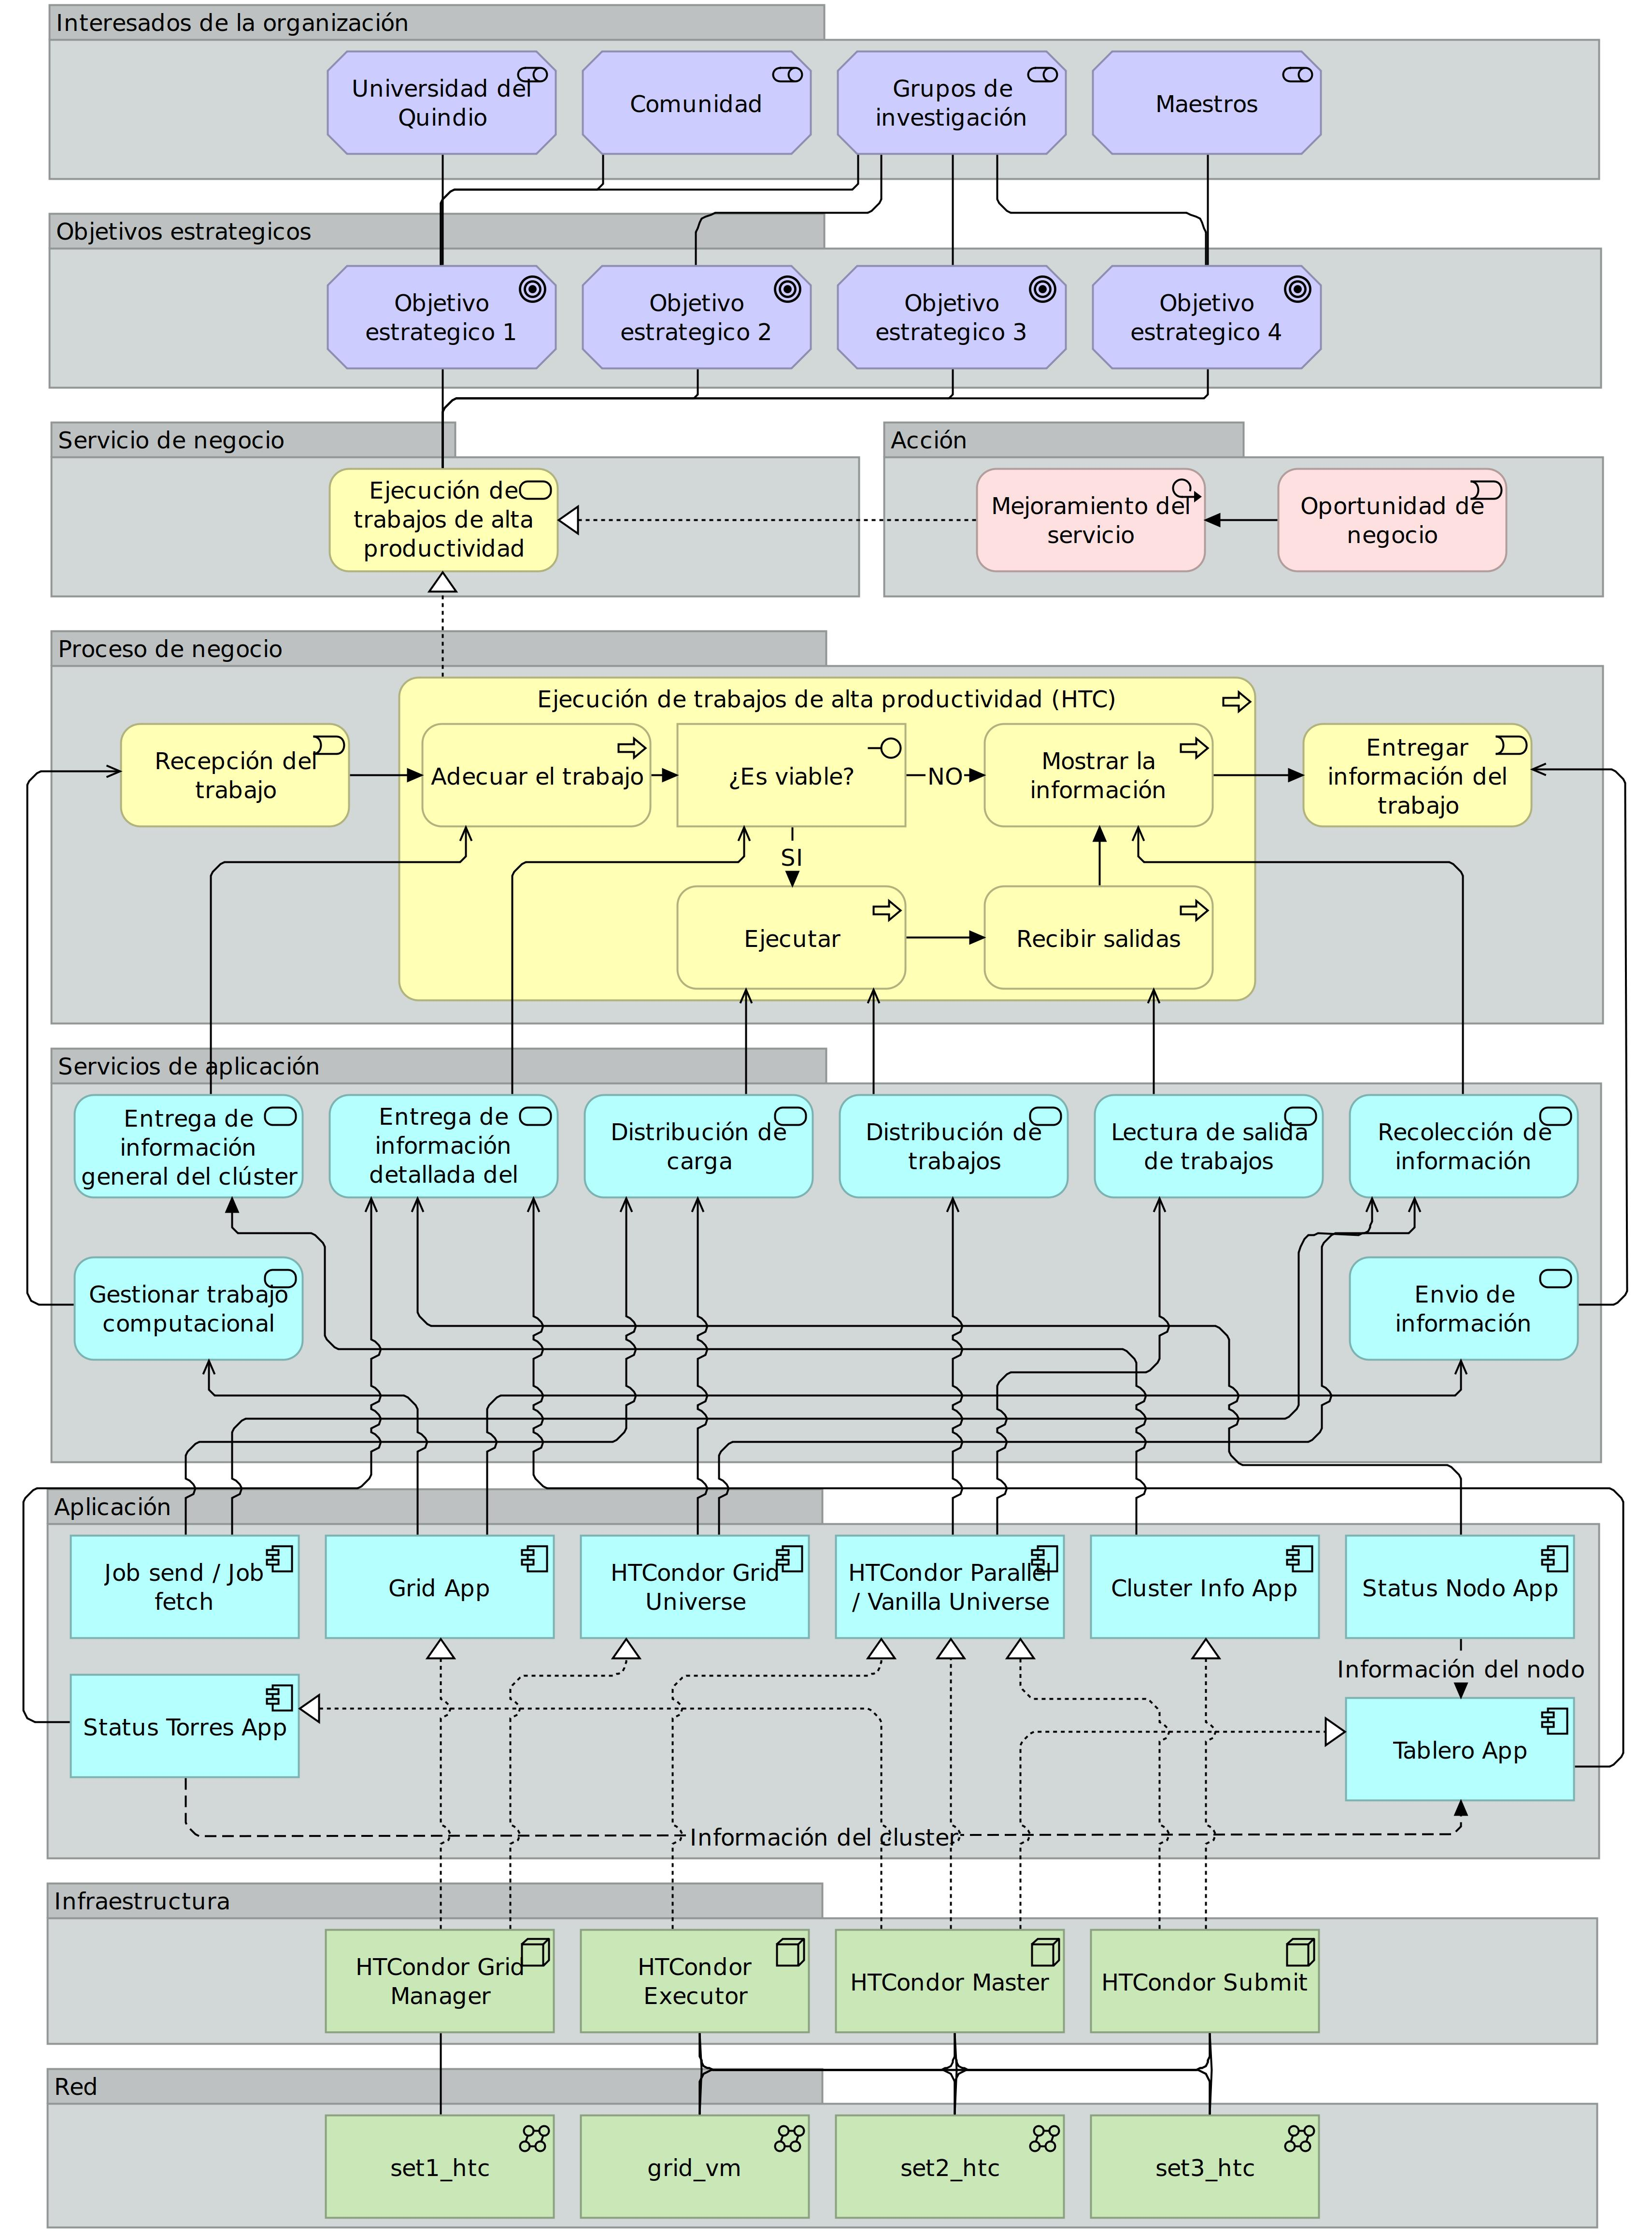
\includegraphics[scale=0.125]{tablas-images/archi/Layered View.jpg}
	\caption{Vista por capas}
    \label{fig:archiLayeredView}
\end{figure}

\section{Modelado del software con el modelo C4}
\noindent
El modelo C4 es una herramienta que ayuda a los equipos de desarrollo de software a describir y comunicar la arquitectura del software a varios niveles de detalle. De forma general el modelo C4 tiene cuatro niveles, cada una con mayor nivel de detalle que la anterior. Para el caso de uso de este proyecto se optó por usar los tres primeros niveles, ya que se considera que el último nivel no da demasiado detalle visual para representar las interacciones en el ámbito de código, por lo que para este fin se usará otro diagrama presentado más adelante.

\subsection{Nivel 1: Diagrama de contexto del sistema}
\noindent
El diagrama de contexto del sistema muestra de forma muy general y a muy alto nivel la solución que se propone. Lo que permite una visión global y generalizada, útil para comprender rápidamente los elementos de la solución.

En la Figura \ref{fig:C4Nivel1} se muestra los elementos principales de la arquitectura, los nombres de dichos elementos, la interacción entre ellos y la comunicación que realizan con el usuario. Como se puede apreciar en el diagrama, el sistema está compuesto de tres aplicaciones y los tres universos de HTCondor que componen la solución. Cabe aclarar que la aplicación denominada \textit{Tablero App} ya estaba implementada en un clúster antes del inicio de este proyecto. Sin embargo, se adiciona a la arquitectura de la solución, ya que se hizo un esfuerzo para adaptar está en todos los clústeres Vanilla que componen la solución.

\begin{figure}[H]
	\centering
	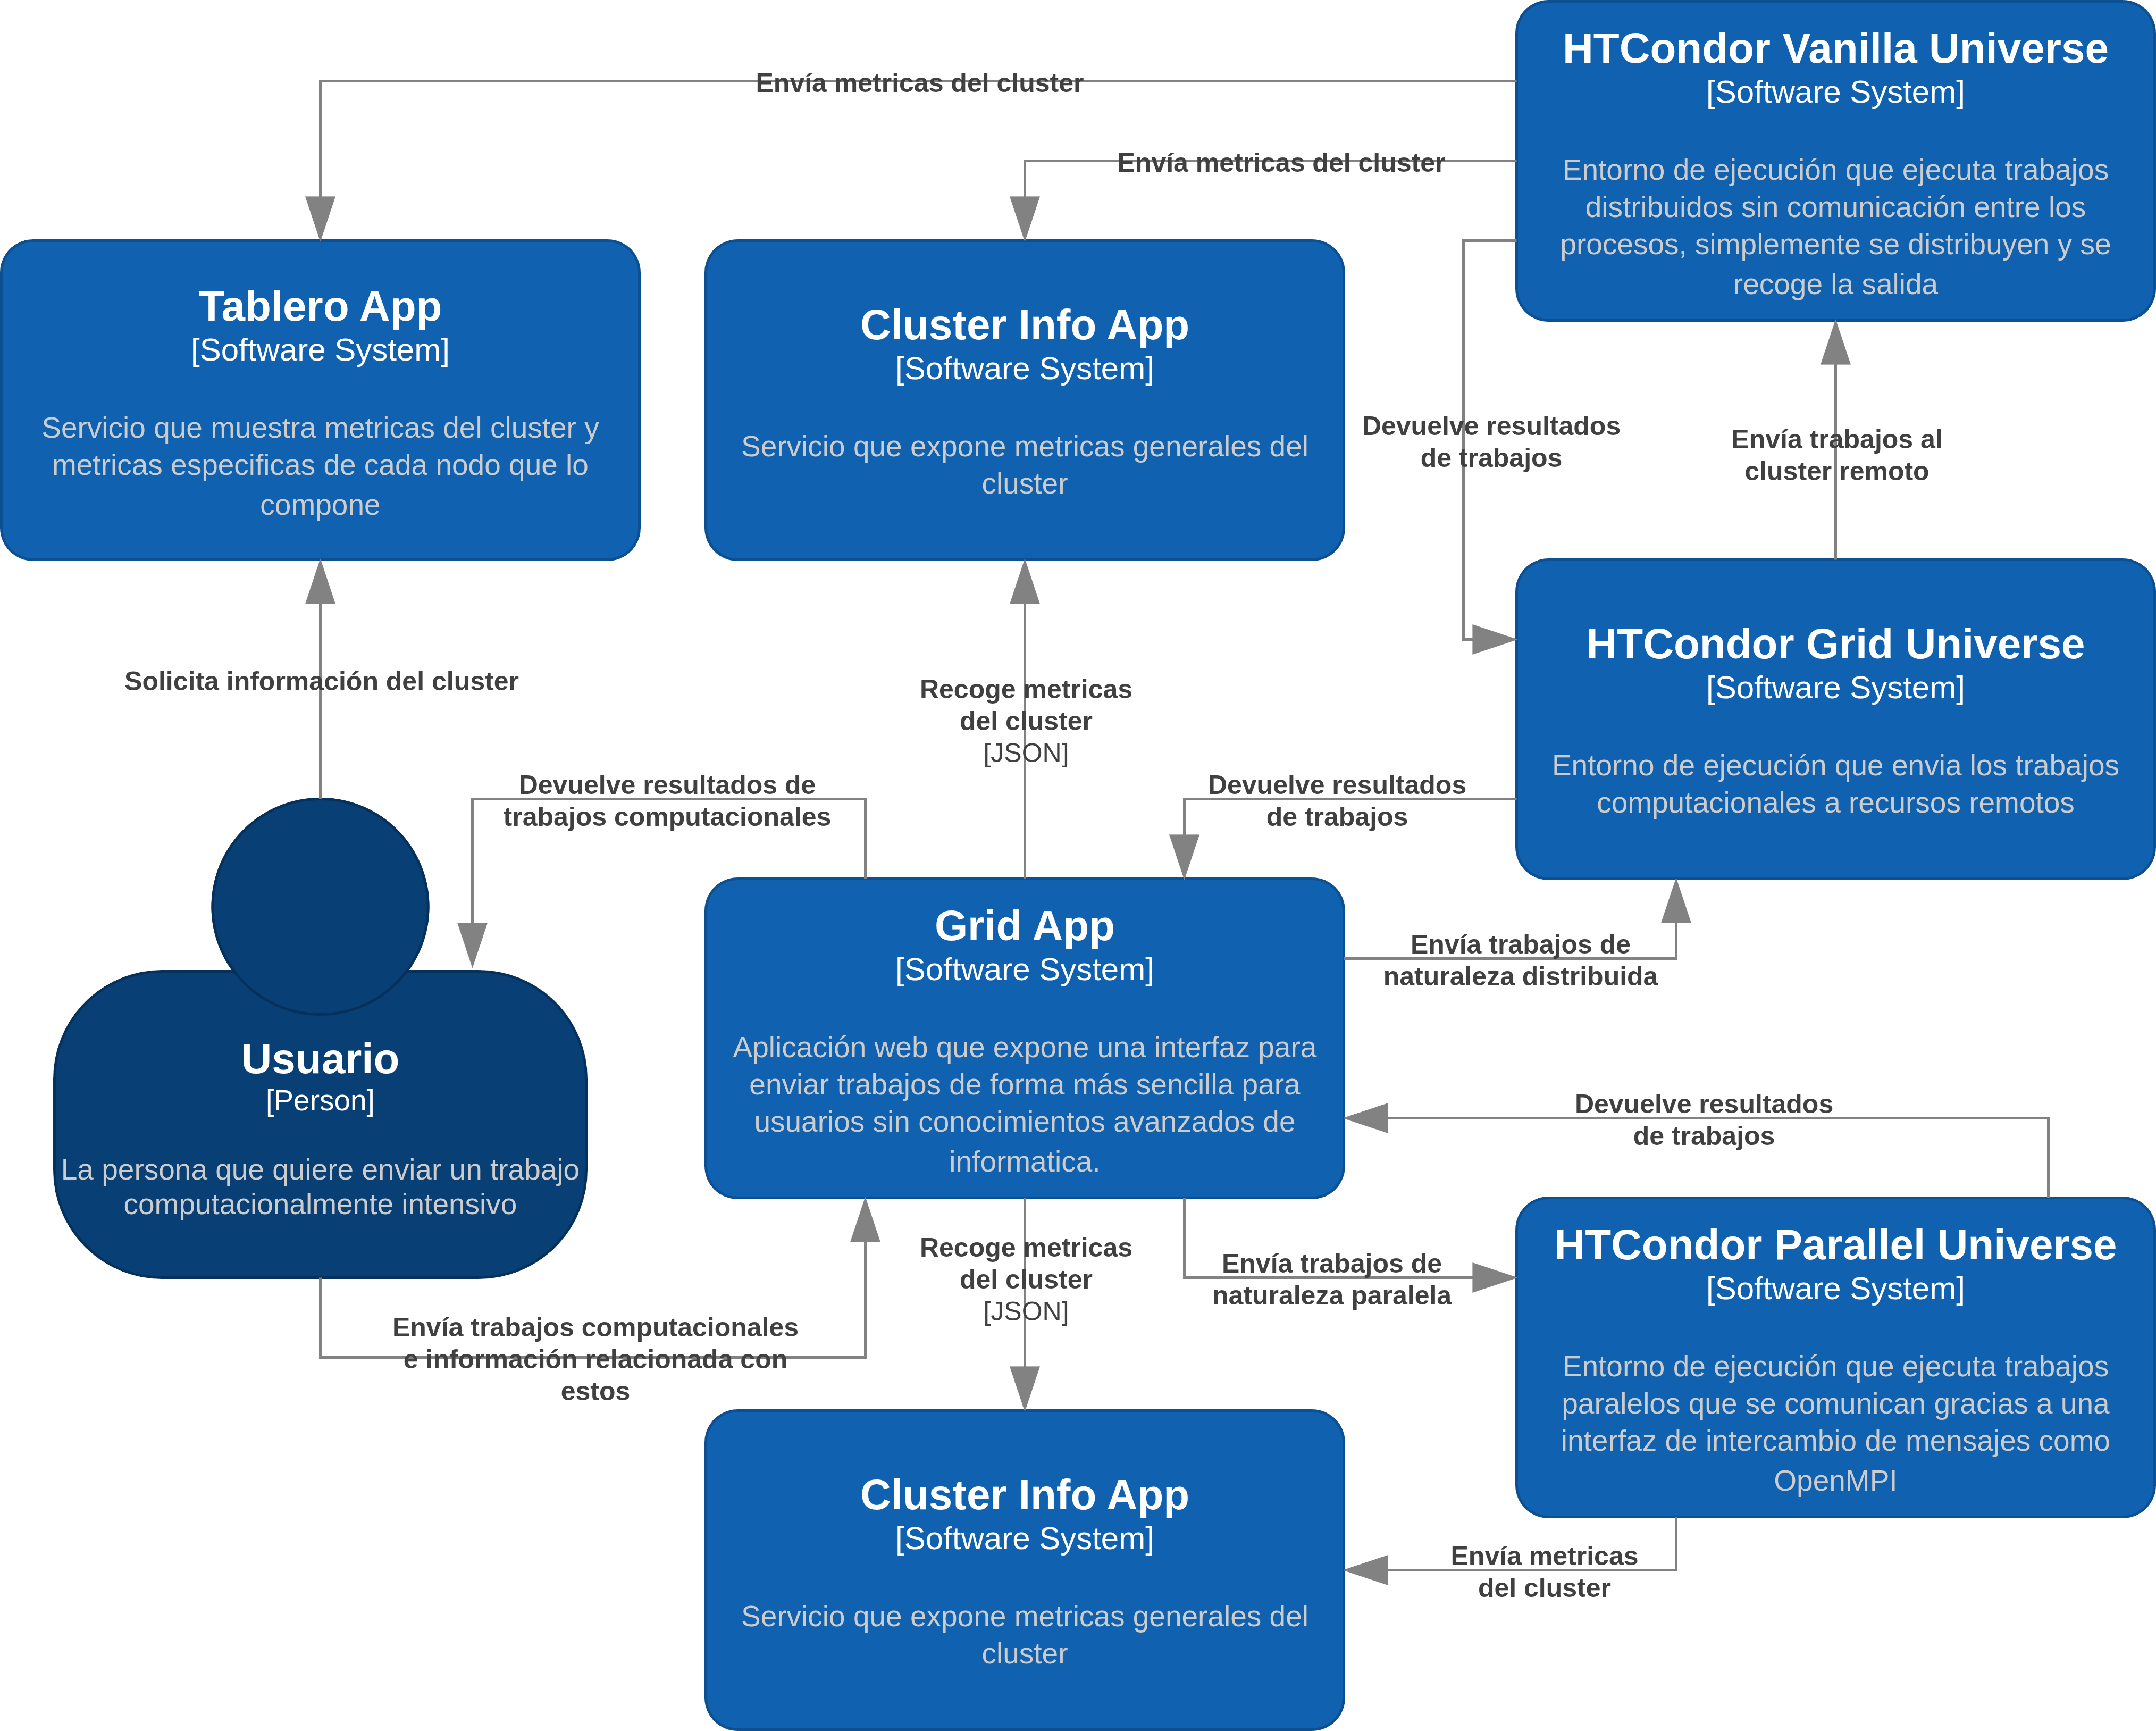
\includegraphics[scale=0.1]{tablas-images/C4/Diagramas HTCondor-Nivel 1.drawio.png}
	\caption{Diagrama de contexto del sistema}
    \label{fig:C4Nivel1}
\end{figure}

\subsection{Nivel 2: Diagrama de contenedores}
\noindent
El diagrama de contenedores muestra los elementos básicos dentro de cada sistema de Software. Lo que permite ir un poco más allá y entender como funciona cada sistema de software por dentro y como interactúa con el resto de contenedores.

En la Figura \ref{fig:C4Nivel2} se muestran los contenedores principales de la arquitectura, los nombres de dichos contenedores, la interacción entre ellos y la comunicación que realizan con el usuario. Como se puede apreciar en el diagrama, el sistema está compuesto por: (1) Un \textit{backend} que cumple dos funciones principales; la primera es renderizar las plantillas que se le van a mostrar al usuario pues estás contienen información dinámica que debe ser consultada y establecida por el servidor, la segunda es realizar toda la lógica de la aplicación como despertar otros procesos o construir los archivos maestros de HTCondor. Se optó por este enfoque en el diseño para propender por la simplicidad de la aplicación y su fácil portabilidad y despliegue en diferentes tipos de entornos. En el Apéndice XX se muestra el código de los componentes y la estructura de los directorios de este componente. (2) Un directorio dentro del sistema de archivos del equipo que sirve la aplicación \textit{Grid App} en donde se almacenan los resultados de los trabajos. (3) Los universos de HTCondor que se propusieron implementar en este proyecto, estos son, Parallel y Grid, pues el Vanilla ya estaba implementado y (4) una aplicación llamada \textit{Cluster Info App} en cada clúster de HTCondor que recoge métricas básicas y las expone en formato \JSON a través de una \API.

\begin{figure}[H]
	\centering
	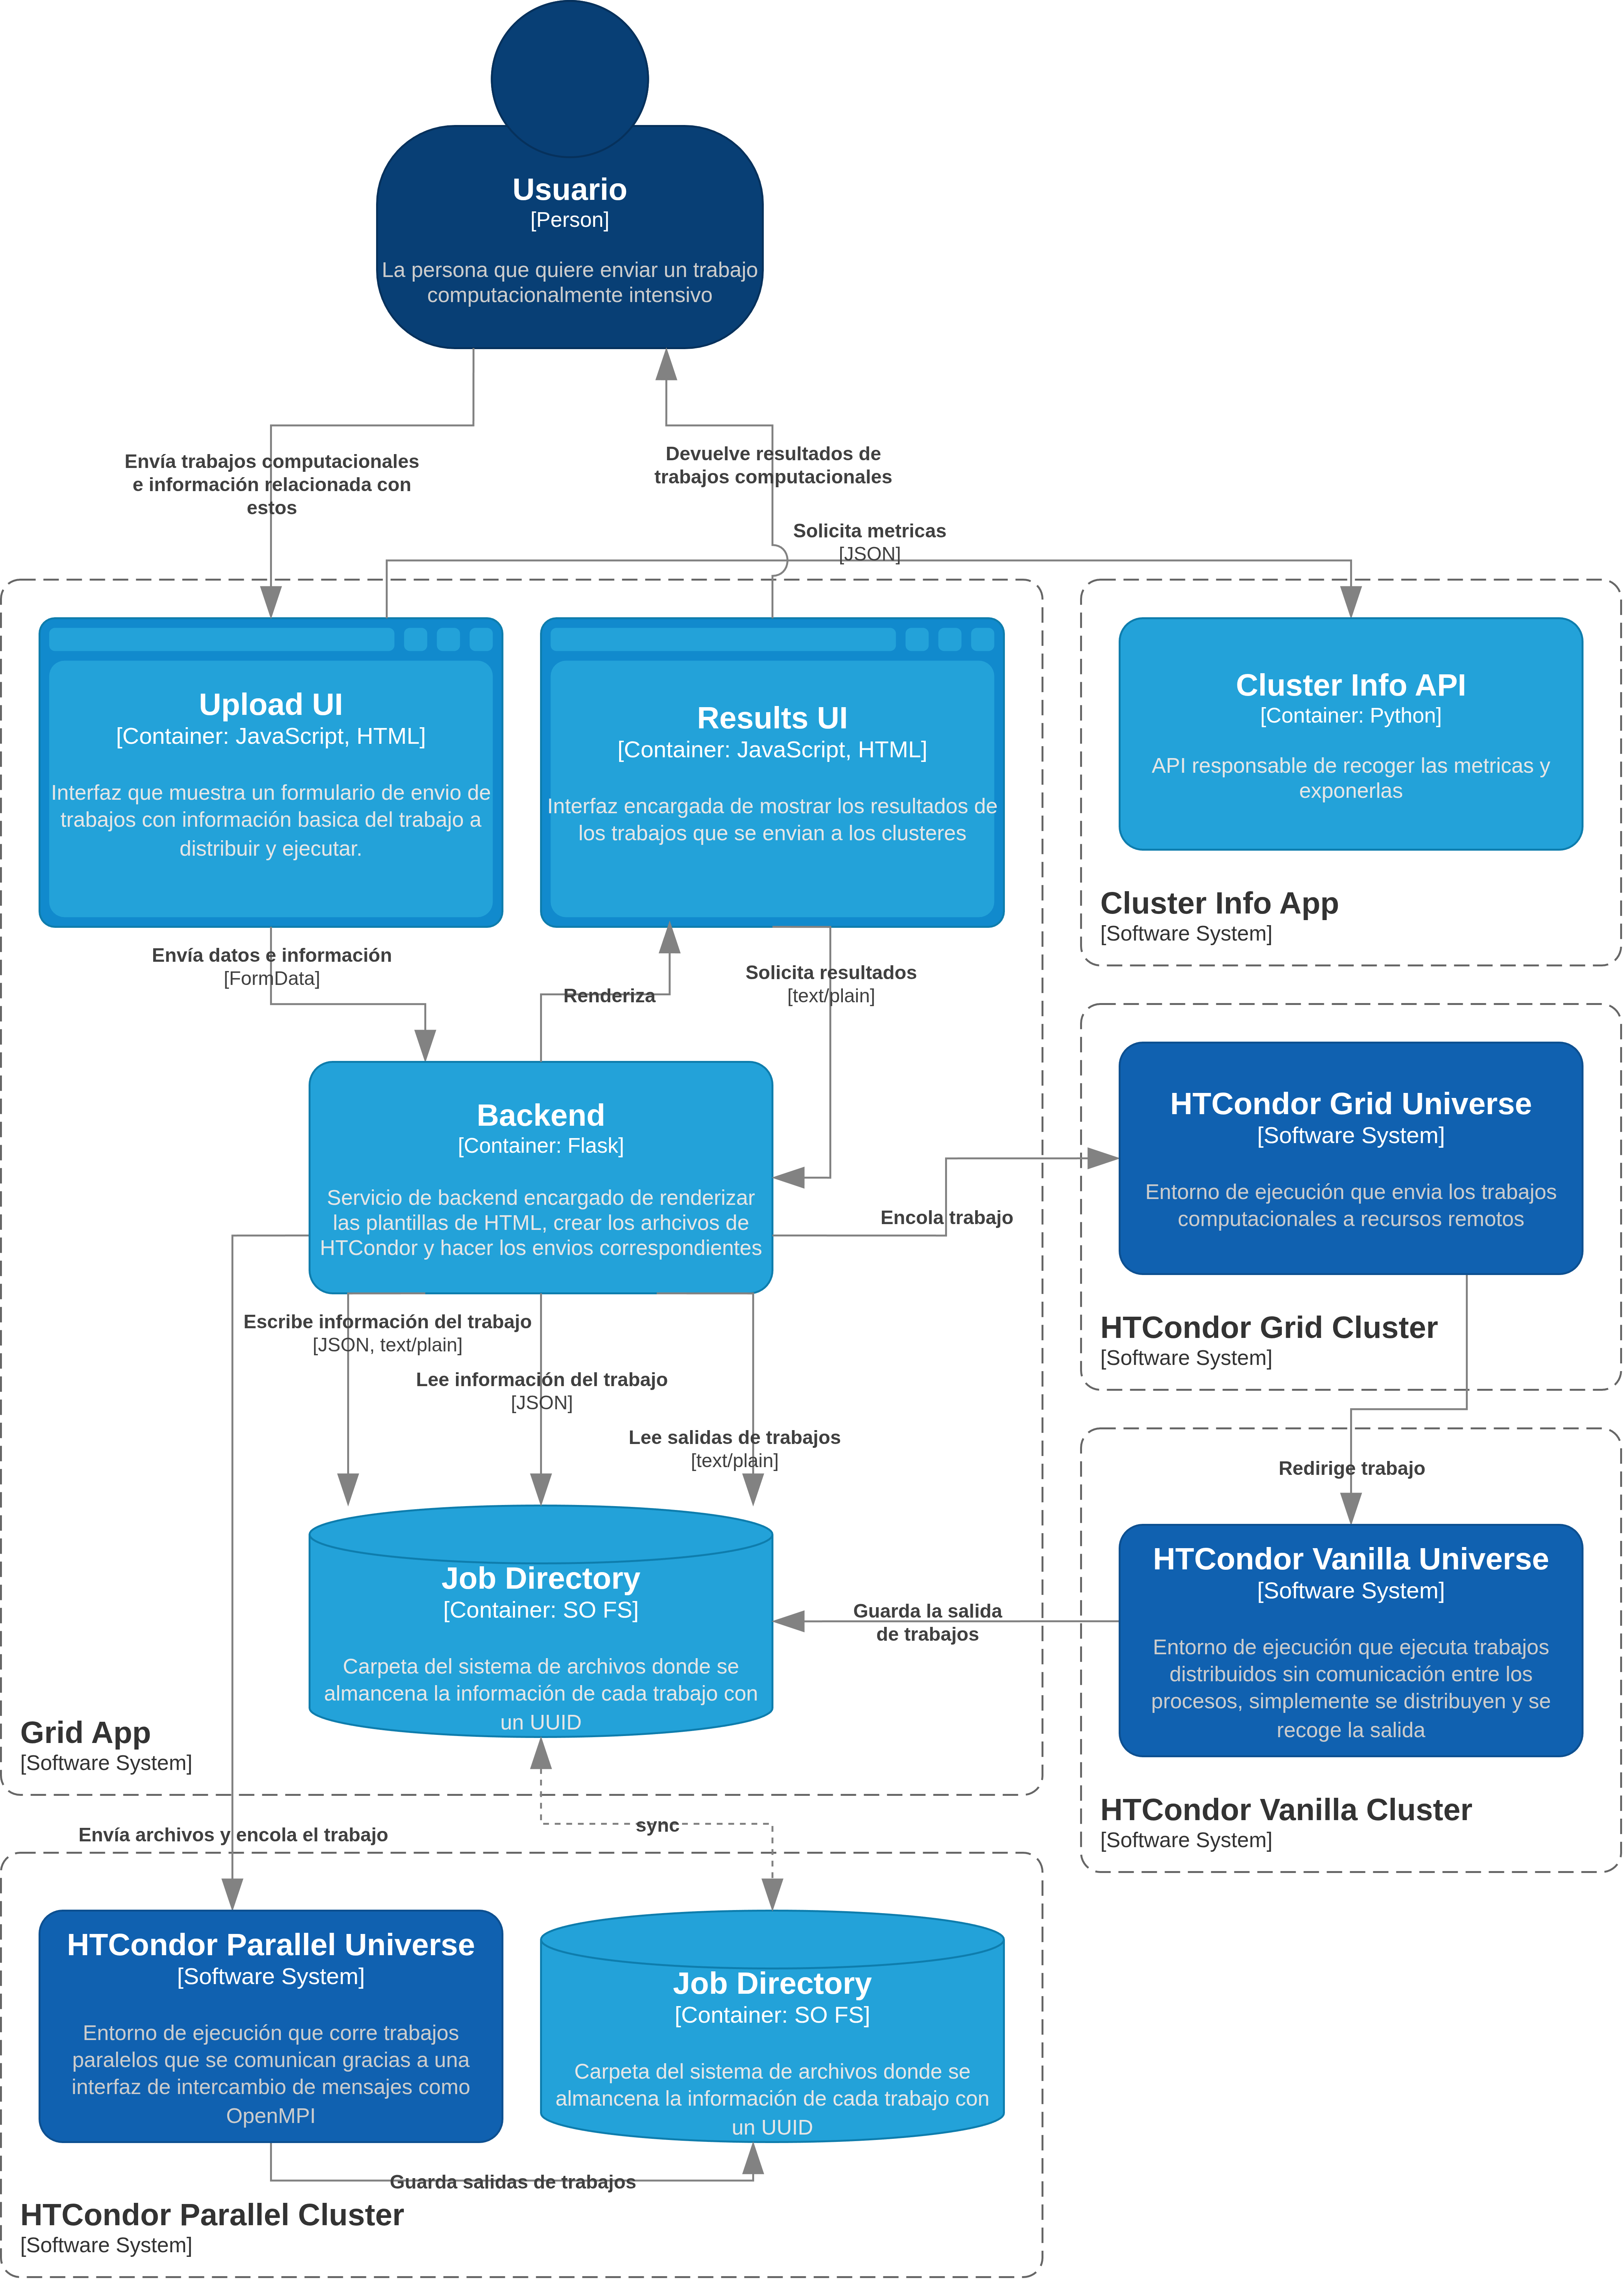
\includegraphics[scale=0.1]{tablas-images/C4/Diagramas HTCondor-Nivel 2.drawio.png}
	\caption{Diagrama de contenedores}
    \label{fig:C4Nivel2}
\end{figure}

\subsection{Nivel 3: Diagrama de componentes}
\noindent
El diagrama de componentes muestra los elementos básicos dentro de cada contenedor. Lo que permite ir aún más allá y entender de forma profunda como están compuestos los elementos del Software y que realizan a nivel interno. Para este nivel de granularidad se decide dividir el diagrama de componentes en distintas partes. Con el fin de hacer más sencilla su lectura y comprensión.

\subsubsection{Universo \textit{Vanilla}}
\noindent
En la Figura \ref{fig:C4Nivel3Vanilla} se muestran los componentes principales de la arquitectura del universo Vanilla en HTCondor. Además, se pueden apreciar los distintos procesos que sigue un trabajo desde su envío hasta la recepción de sus resultados.

\begin{figure}[H]
	\centering
	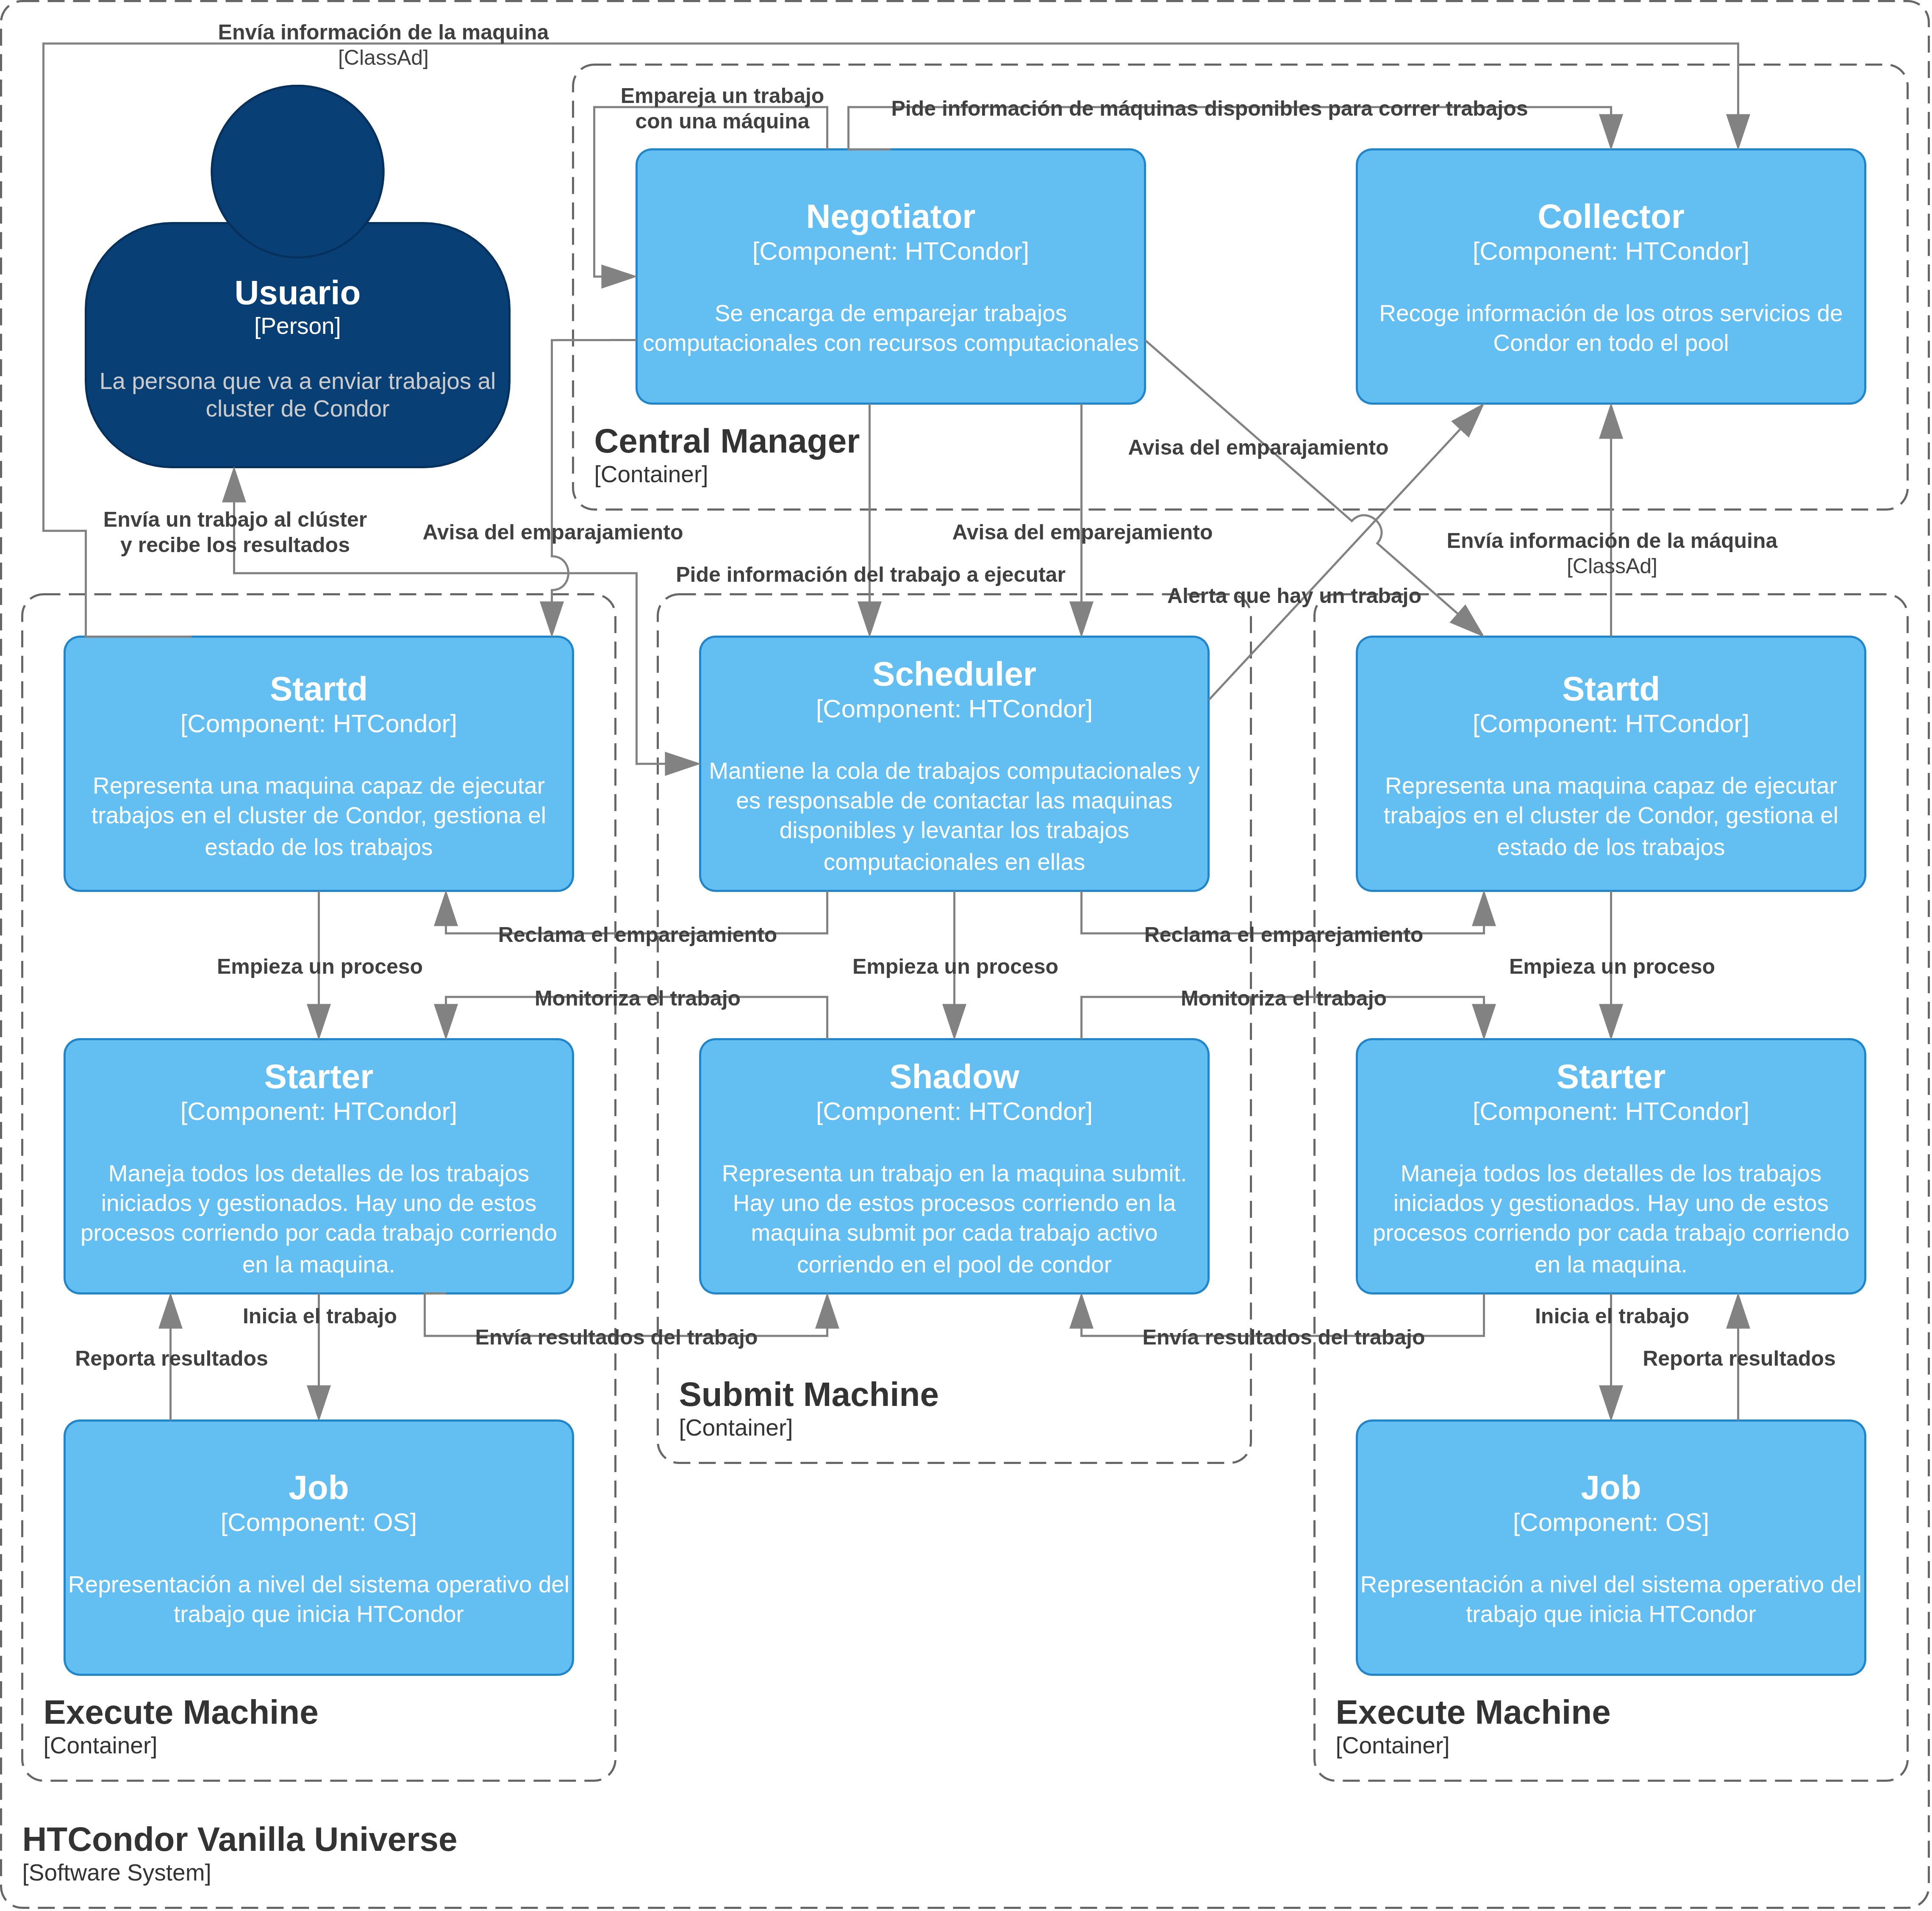
\includegraphics[scale=0.09]{tablas-images/C4/Diagramas HTCondor-Nivel 3 - Vanilla.drawio.png}
	\caption{Diagrama de componentes para el universo Vanilla}
    \label{fig:C4Nivel3Vanilla}
\end{figure}

\subsubsection{Universo \textit{Parallel}}
\noindent
En la Figura \ref{fig:C4Nivel3Parallel} se muestran los componentes principales de la arquitectura del universo Parallel en HTCondor. Además, se pueden apreciar los distintos procesos que sigue un trabajo desde su envío hasta la recepción de sus resultados. Es importante notar que ls comunicación y los componentes funcionan exactamente de la misma forma que en el universo Vanilla, con la unica diferencia que aquí, los trabajo se comunican a través de \MPI.

\begin{figure}[H]
	\centering
	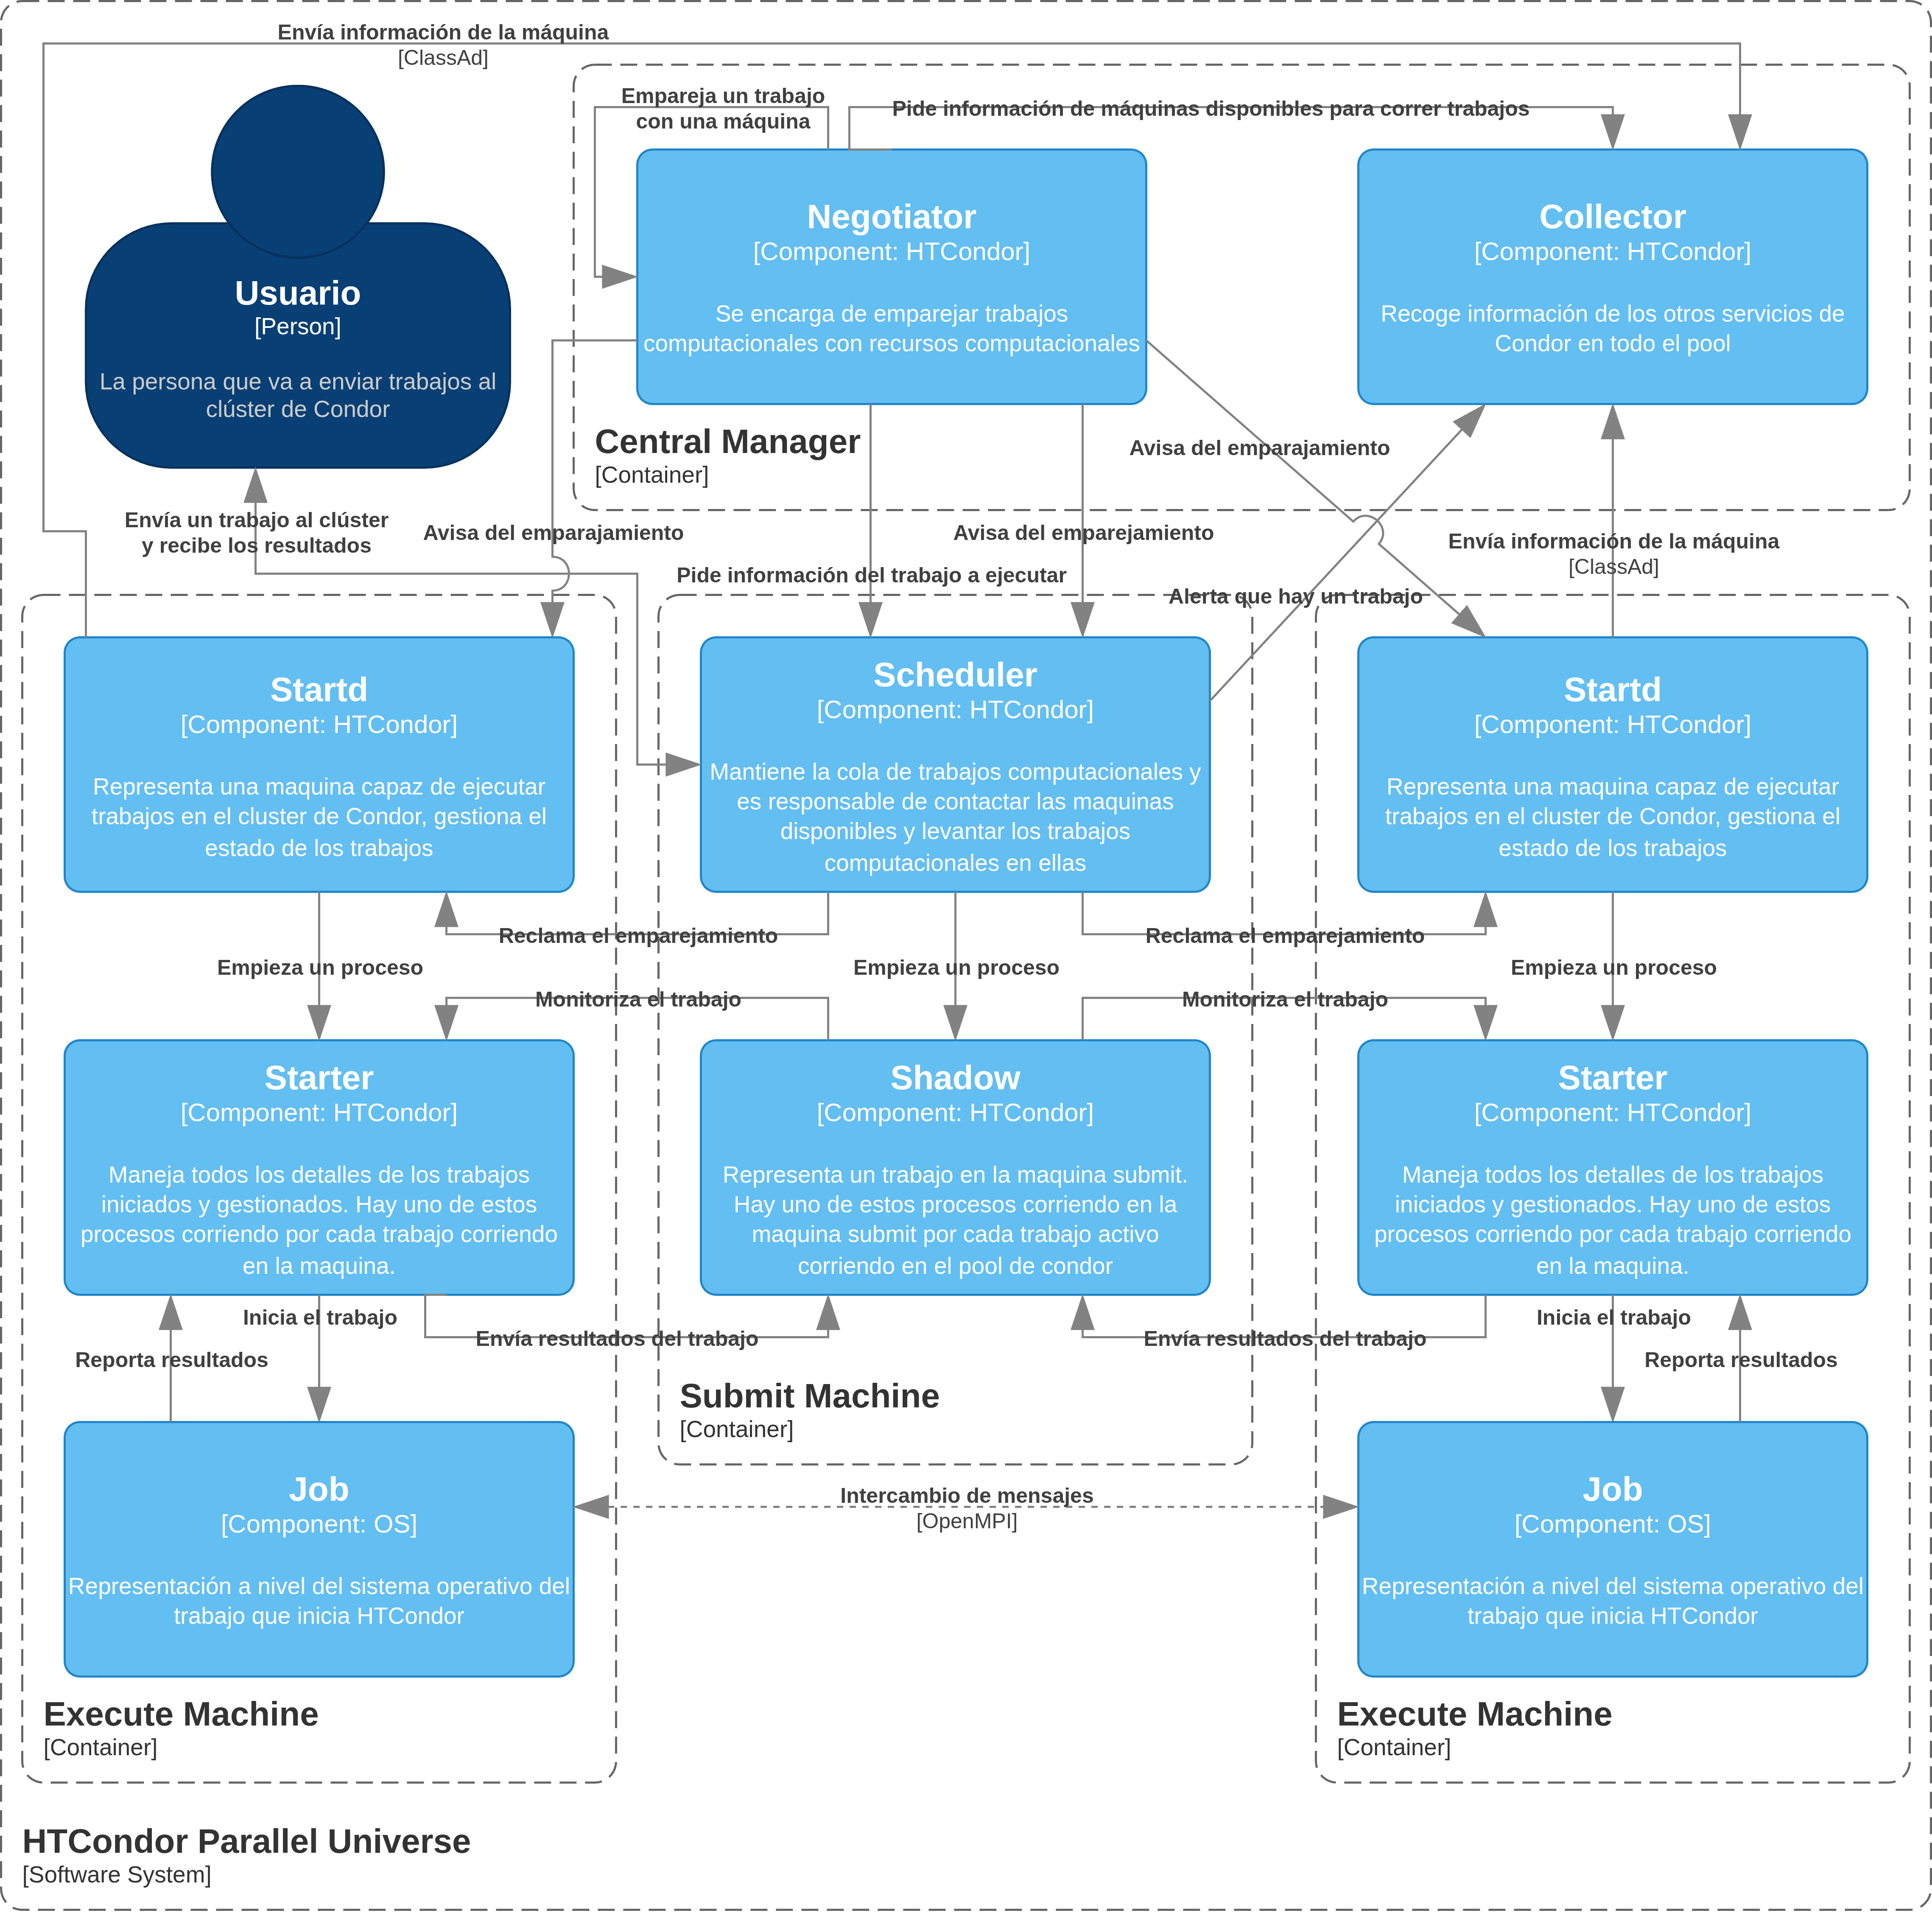
\includegraphics[scale=0.09]{tablas-images/C4/Diagramas HTCondor-Nivel 3 - Parallel.drawio.png}
	\caption{Diagrama de componentes para el universo Parallel}
    \label{fig:C4Nivel3Parallel}
\end{figure}

\subsubsection{Universo \textit{Grid}}
\noindent
En la Figura \ref{fig:C4Nivel3Grid} se muestran los componentes principales de la arquitectura del universo Grid en HTCondor. Como se puede apreciar en el digrama este universo actua como un intermediario entre el usuario y el clúster que va a ejecutar su trabajo, permitiendo así interconectar multiples clústeres, donde reside el valor de este universo.

\begin{figure}[H]
	\centering
	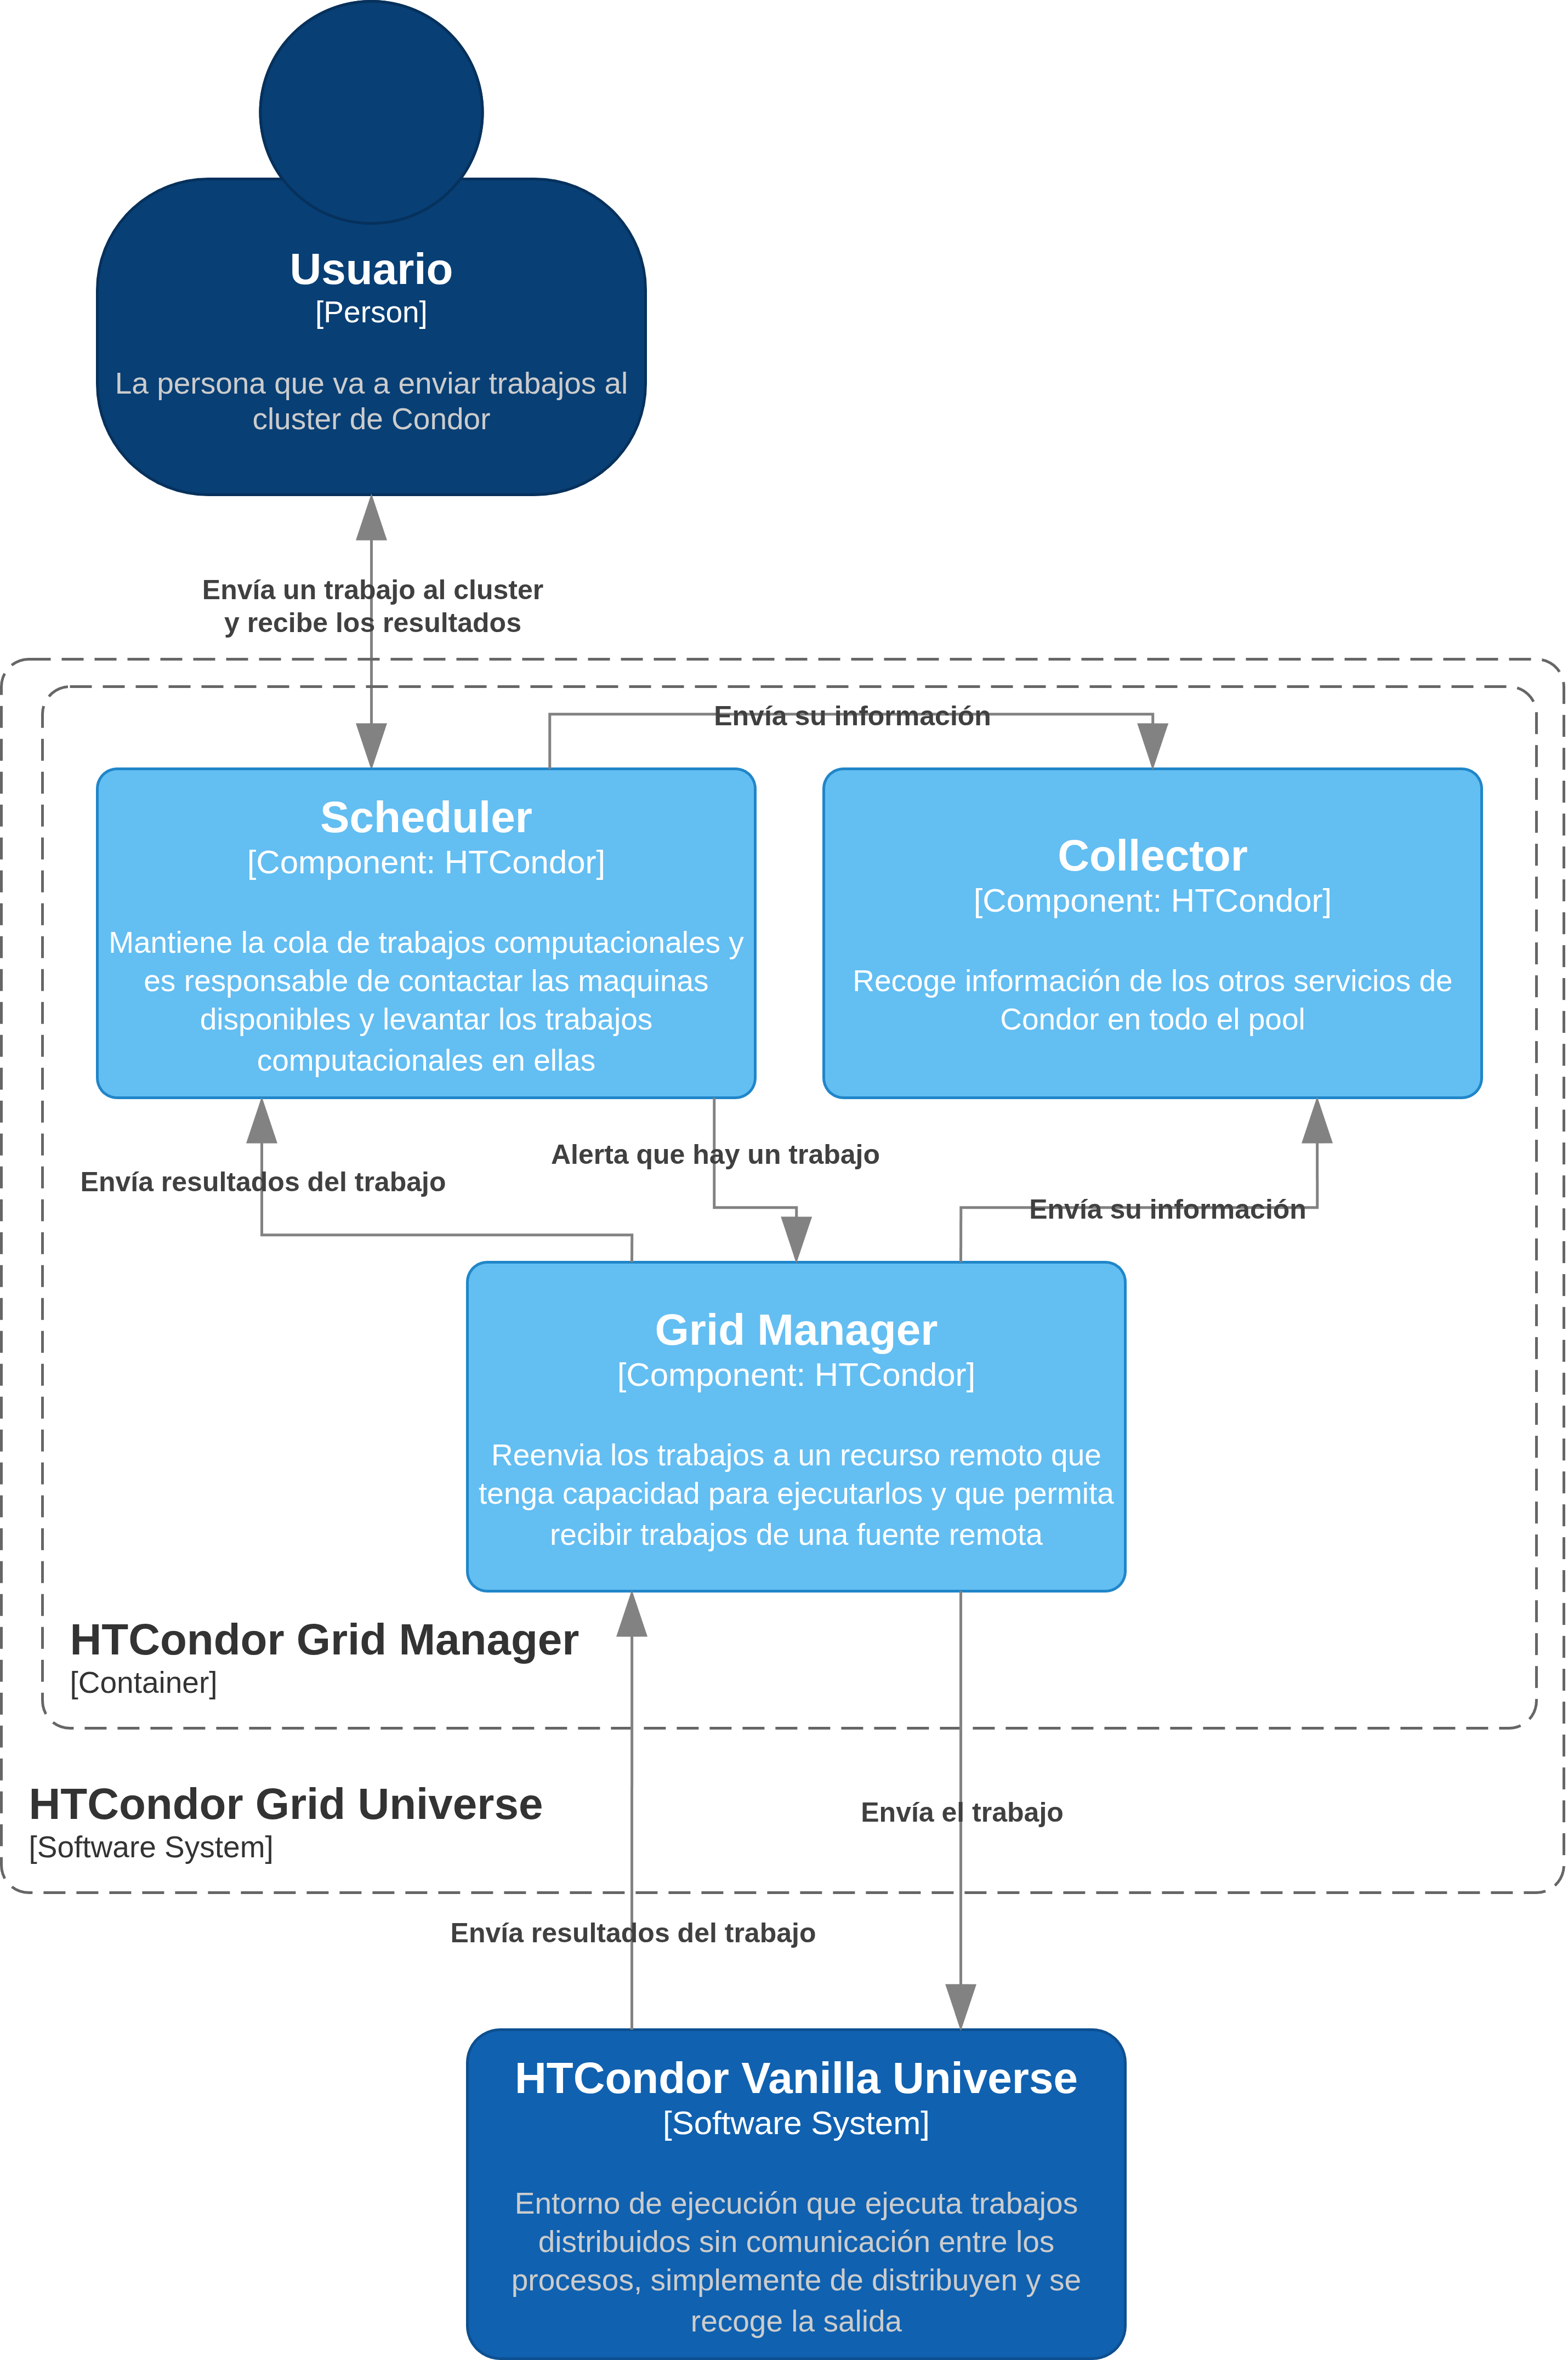
\includegraphics[scale=0.1]{tablas-images/C4/Diagramas HTCondor-Nivel 3 - Grid.drawio.png}
	\caption{Diagrama de componentes para el universo Grid}
    \label{fig:C4Nivel3Grid}
\end{figure}

\subsubsection{Aplicaciones de Software}
\noindent
En la Figura \ref{fig:C4Nivel3Apps} se muestran los componentes principales de las aplicaciones que integran el sistema. Como se puede evidenciar en el diagrama, hay dos aplicaciones principales que conforman este sistema. La primera es la aplicación central \textit{Grid App} que ayuda a abstraer la complejidad de HTCondor con una interfaz \textit{web} más amigable, además, es la encargada de enviar los trabajos y recoger los resultados. La segunda es la \textit{Cluster Info App} que ayuda a exponer métricas de cada clúster, permitiendo así a la aplicación central obtener datos reales de cada clúster y permitir al usuario elegir el clúster con métricas más favorables para su caso de uso. Es importante aclarar que la aplicación \textit{Tablero App} también está disponible y funcionando en algunos de los clústeres que componen la solución. Sin embargo, dado que su única labor es mostrar métricas detalladas del clúster, se opta por no agregarlo al diagrama por dos razones: (1) para reducir su complejidad y (2) porque el desarrollo de esta aplicación no es resultado del desarrollo de este proyecto.

\begin{figure}[H]
	\centering
	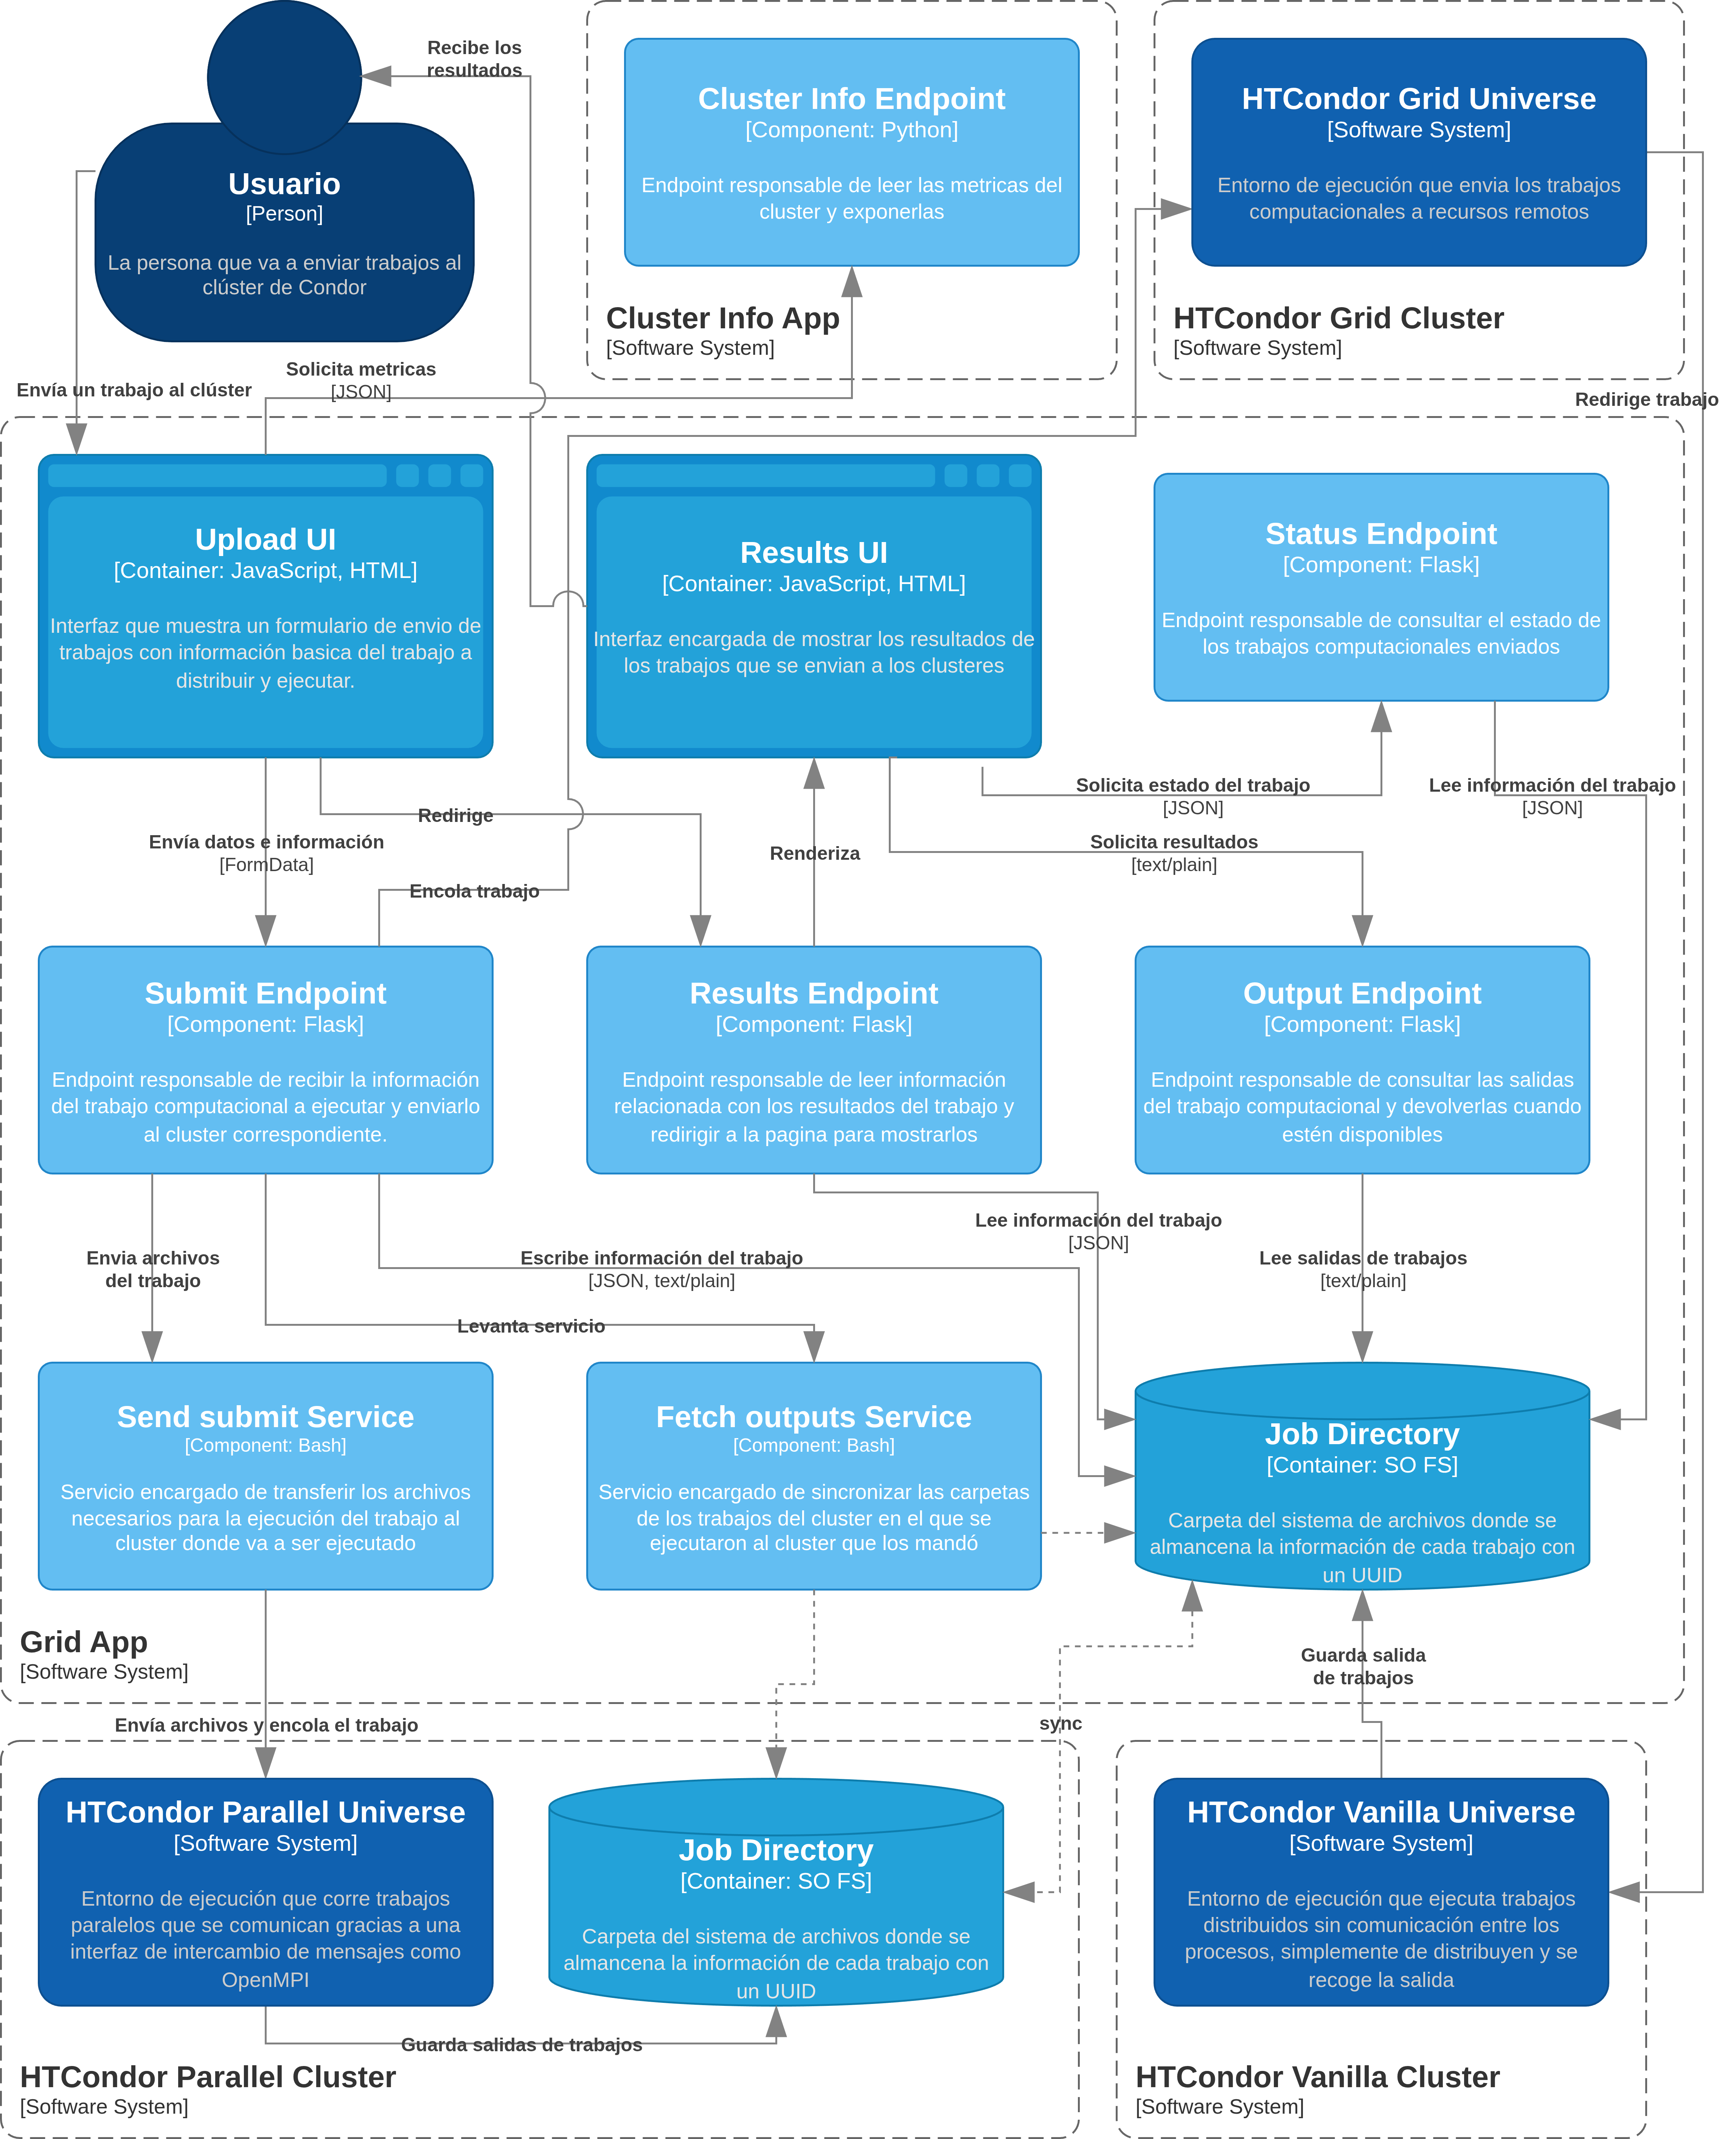
\includegraphics[scale=0.09]{tablas-images/C4/Diagramas HTCondor-Nivel 3 - Apps.drawio.png}
	\caption{Diagrama de componentes para las aplicaciones que componen el sistema}
    \label{fig:C4Nivel3Apps}
\end{figure}

\section{Modelado de secuencia con UML}
\UML es un lenguaje de modelado orientado a múltiples enfoques como la secuencia de eventos y la estructura de las clases \citep{10.1145/1125944.1125949}. Para el caso de este proyecto se usará para describir de forma concreta y estructurada la secuencia que siguen los componentes del Software en cada momento, así como las alternativas que toma el programa con base en la información disponible. De igual forma, se usará este lenguaje para modelar la estructura de las clases que transportan información a través del programa. Cabe aclarar que el sistema no se diseña con una orientación a objetos estricta. Sin embargo su forma principal de intercambio de información es a través de \JSON. Por lo que se hace necesario conocer y describir la forma de los objetos que se intercambian.

\subsection{Diagrama de secuencia}
\noindent
En la Figura \ref{fig:UMLSecuencia} se muestran los procesos y llamados que se ejecutan en cada paso del sistema, desde las rutas que se visitan hasta la información que se transfiere en cada momento. Es importante añadir que la información de transferencia entre cada sistema de software es meramente ilustrativa y para dar mayor profundidad a dicha información, debe complementarse con el diagrama de clases presentado en la sección siguiente y el código de la aplicación presentado en el Apéndice XX.

\begin{figure}[H]
	\centering
	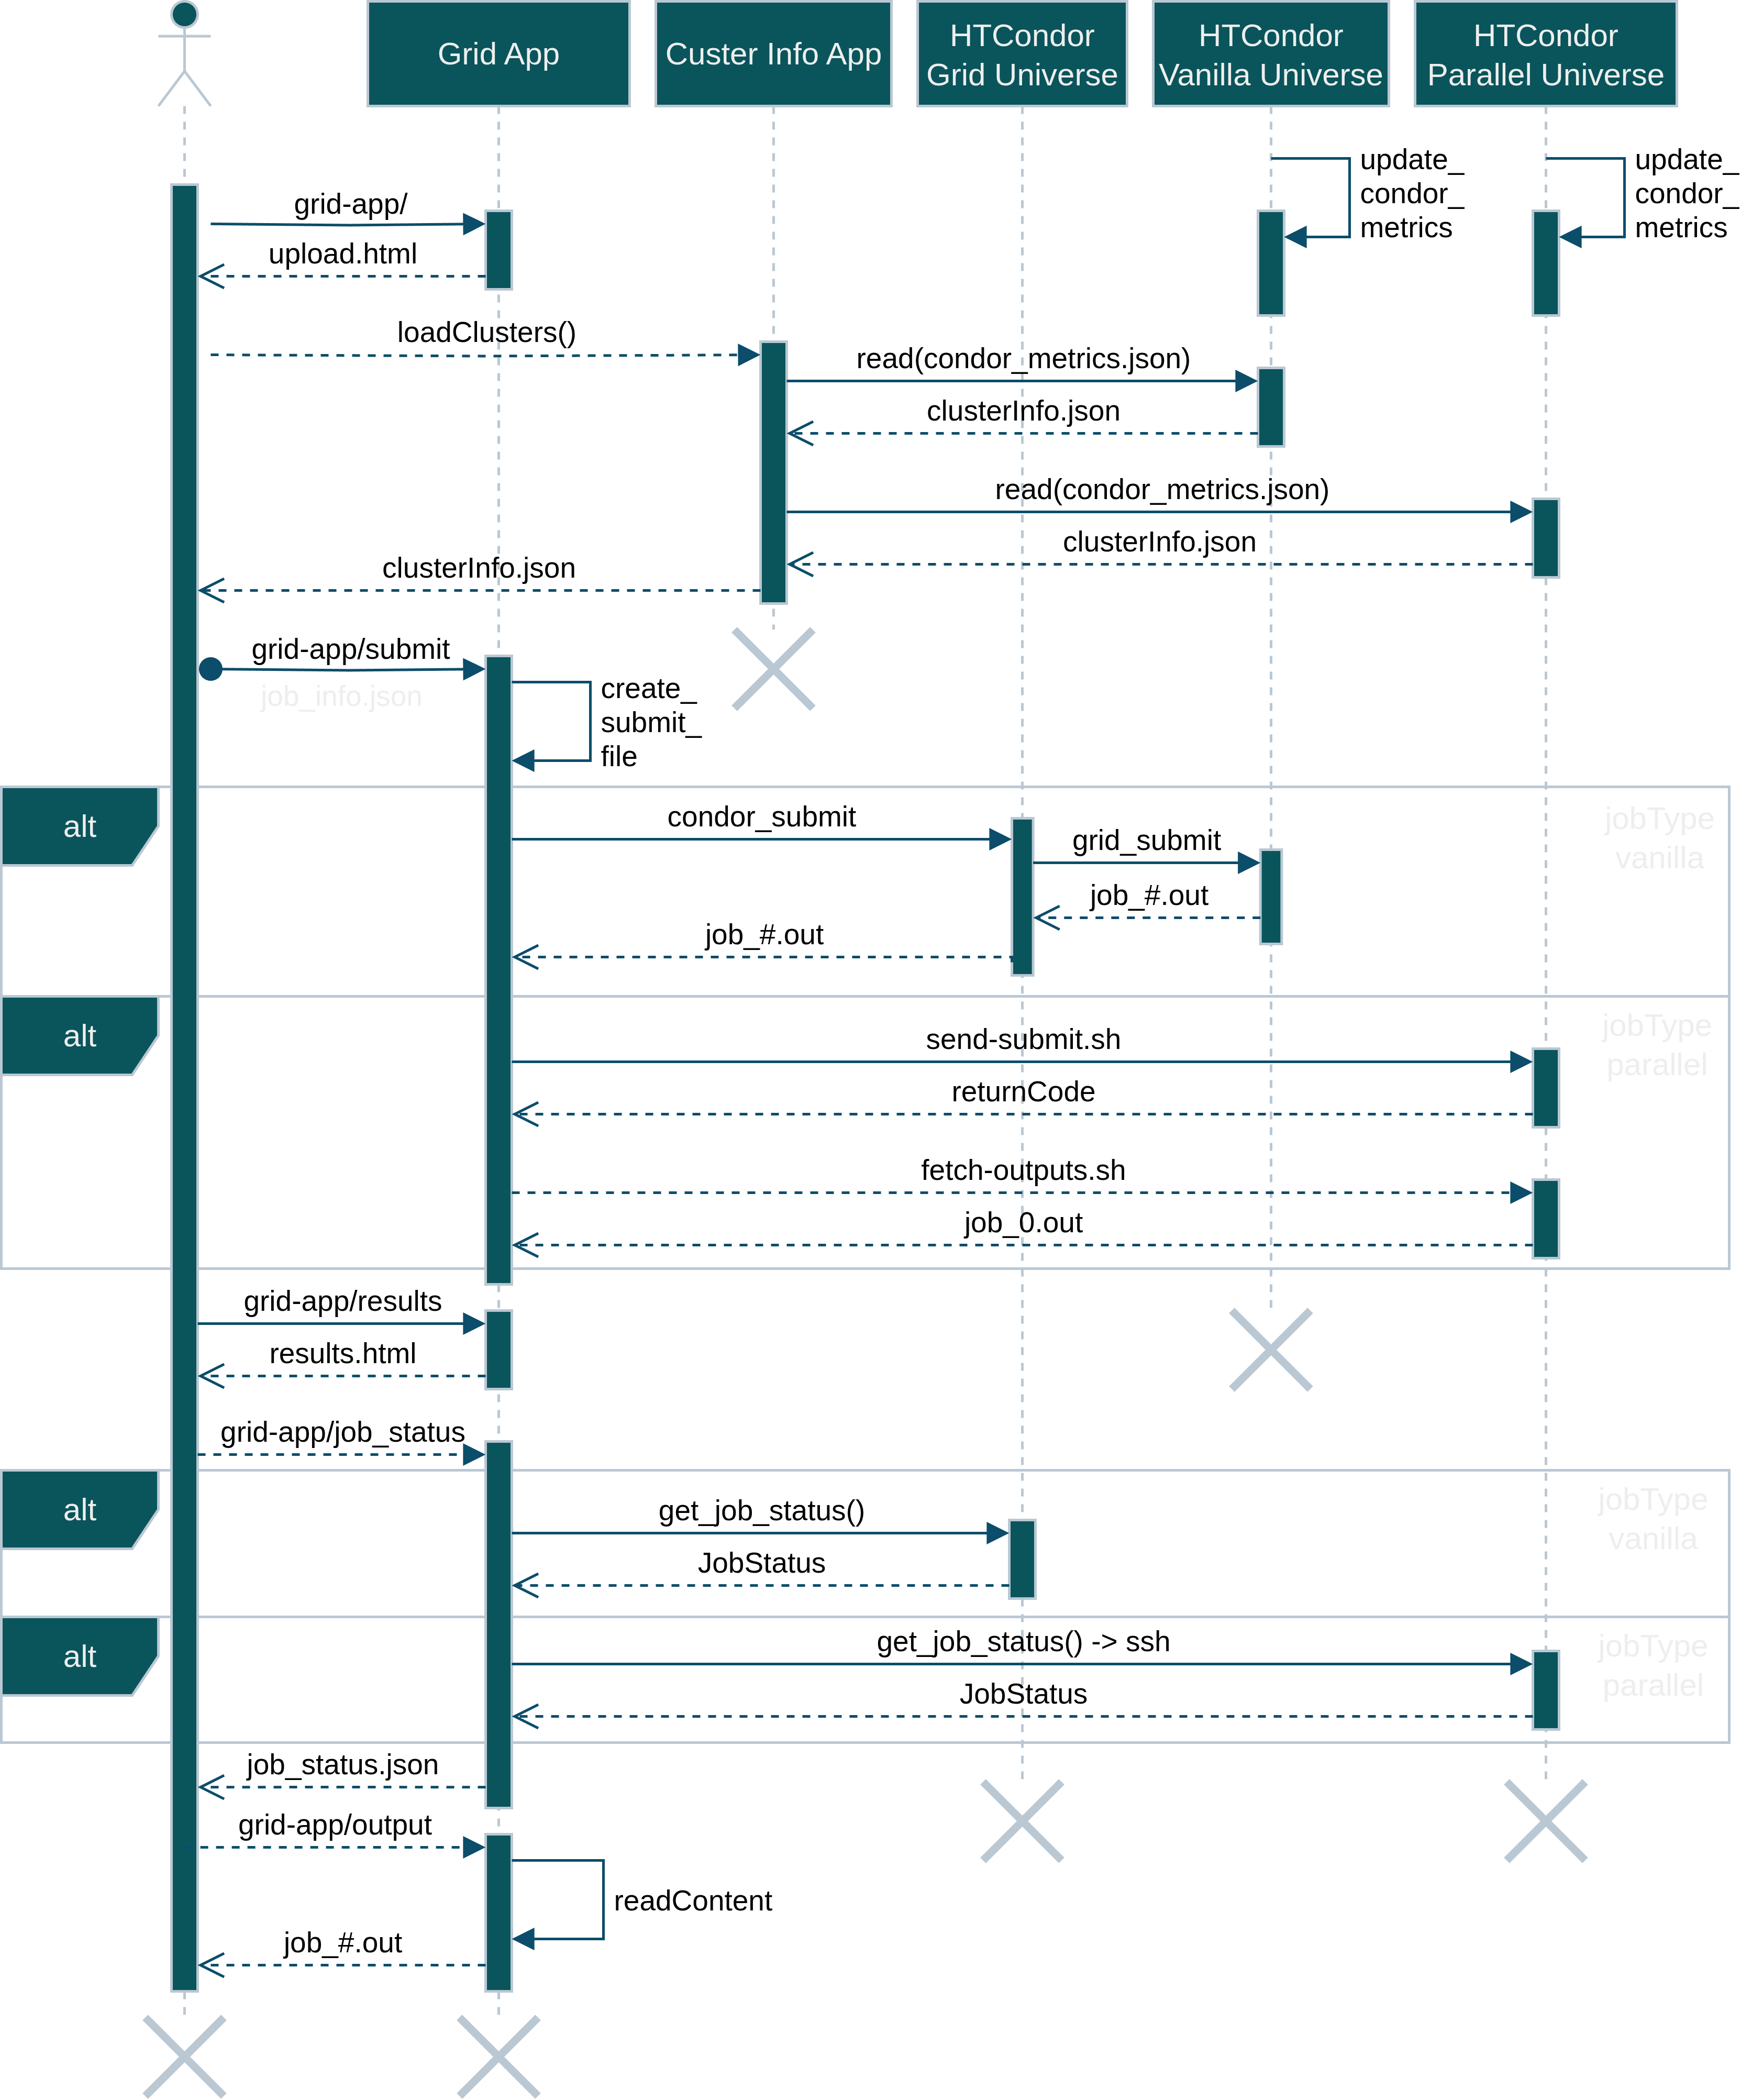
\includegraphics[scale=0.11]{tablas-images/UML/Diagramas HTCondor-Secuencia.drawio.png}
	\caption{Diagrama de secuencia para el sistema}
    \label{fig:UMLSecuencia}
\end{figure}

\subsection{Diagrama de clases}
\noindent
En la Figura \ref{fig:UMLClases} se muestra la composición de las clases en las que se basan los objetos que permiten intercambiar información a través de los sistemas. Debido a que el diseño no fue orientado a objetos, este diagrama solo pretende mostrar los elementos de información que intercambia el sistema y no pretende modelar la arquitectura general de los sistemas de software.

\begin{figure}[H]
	\centering
	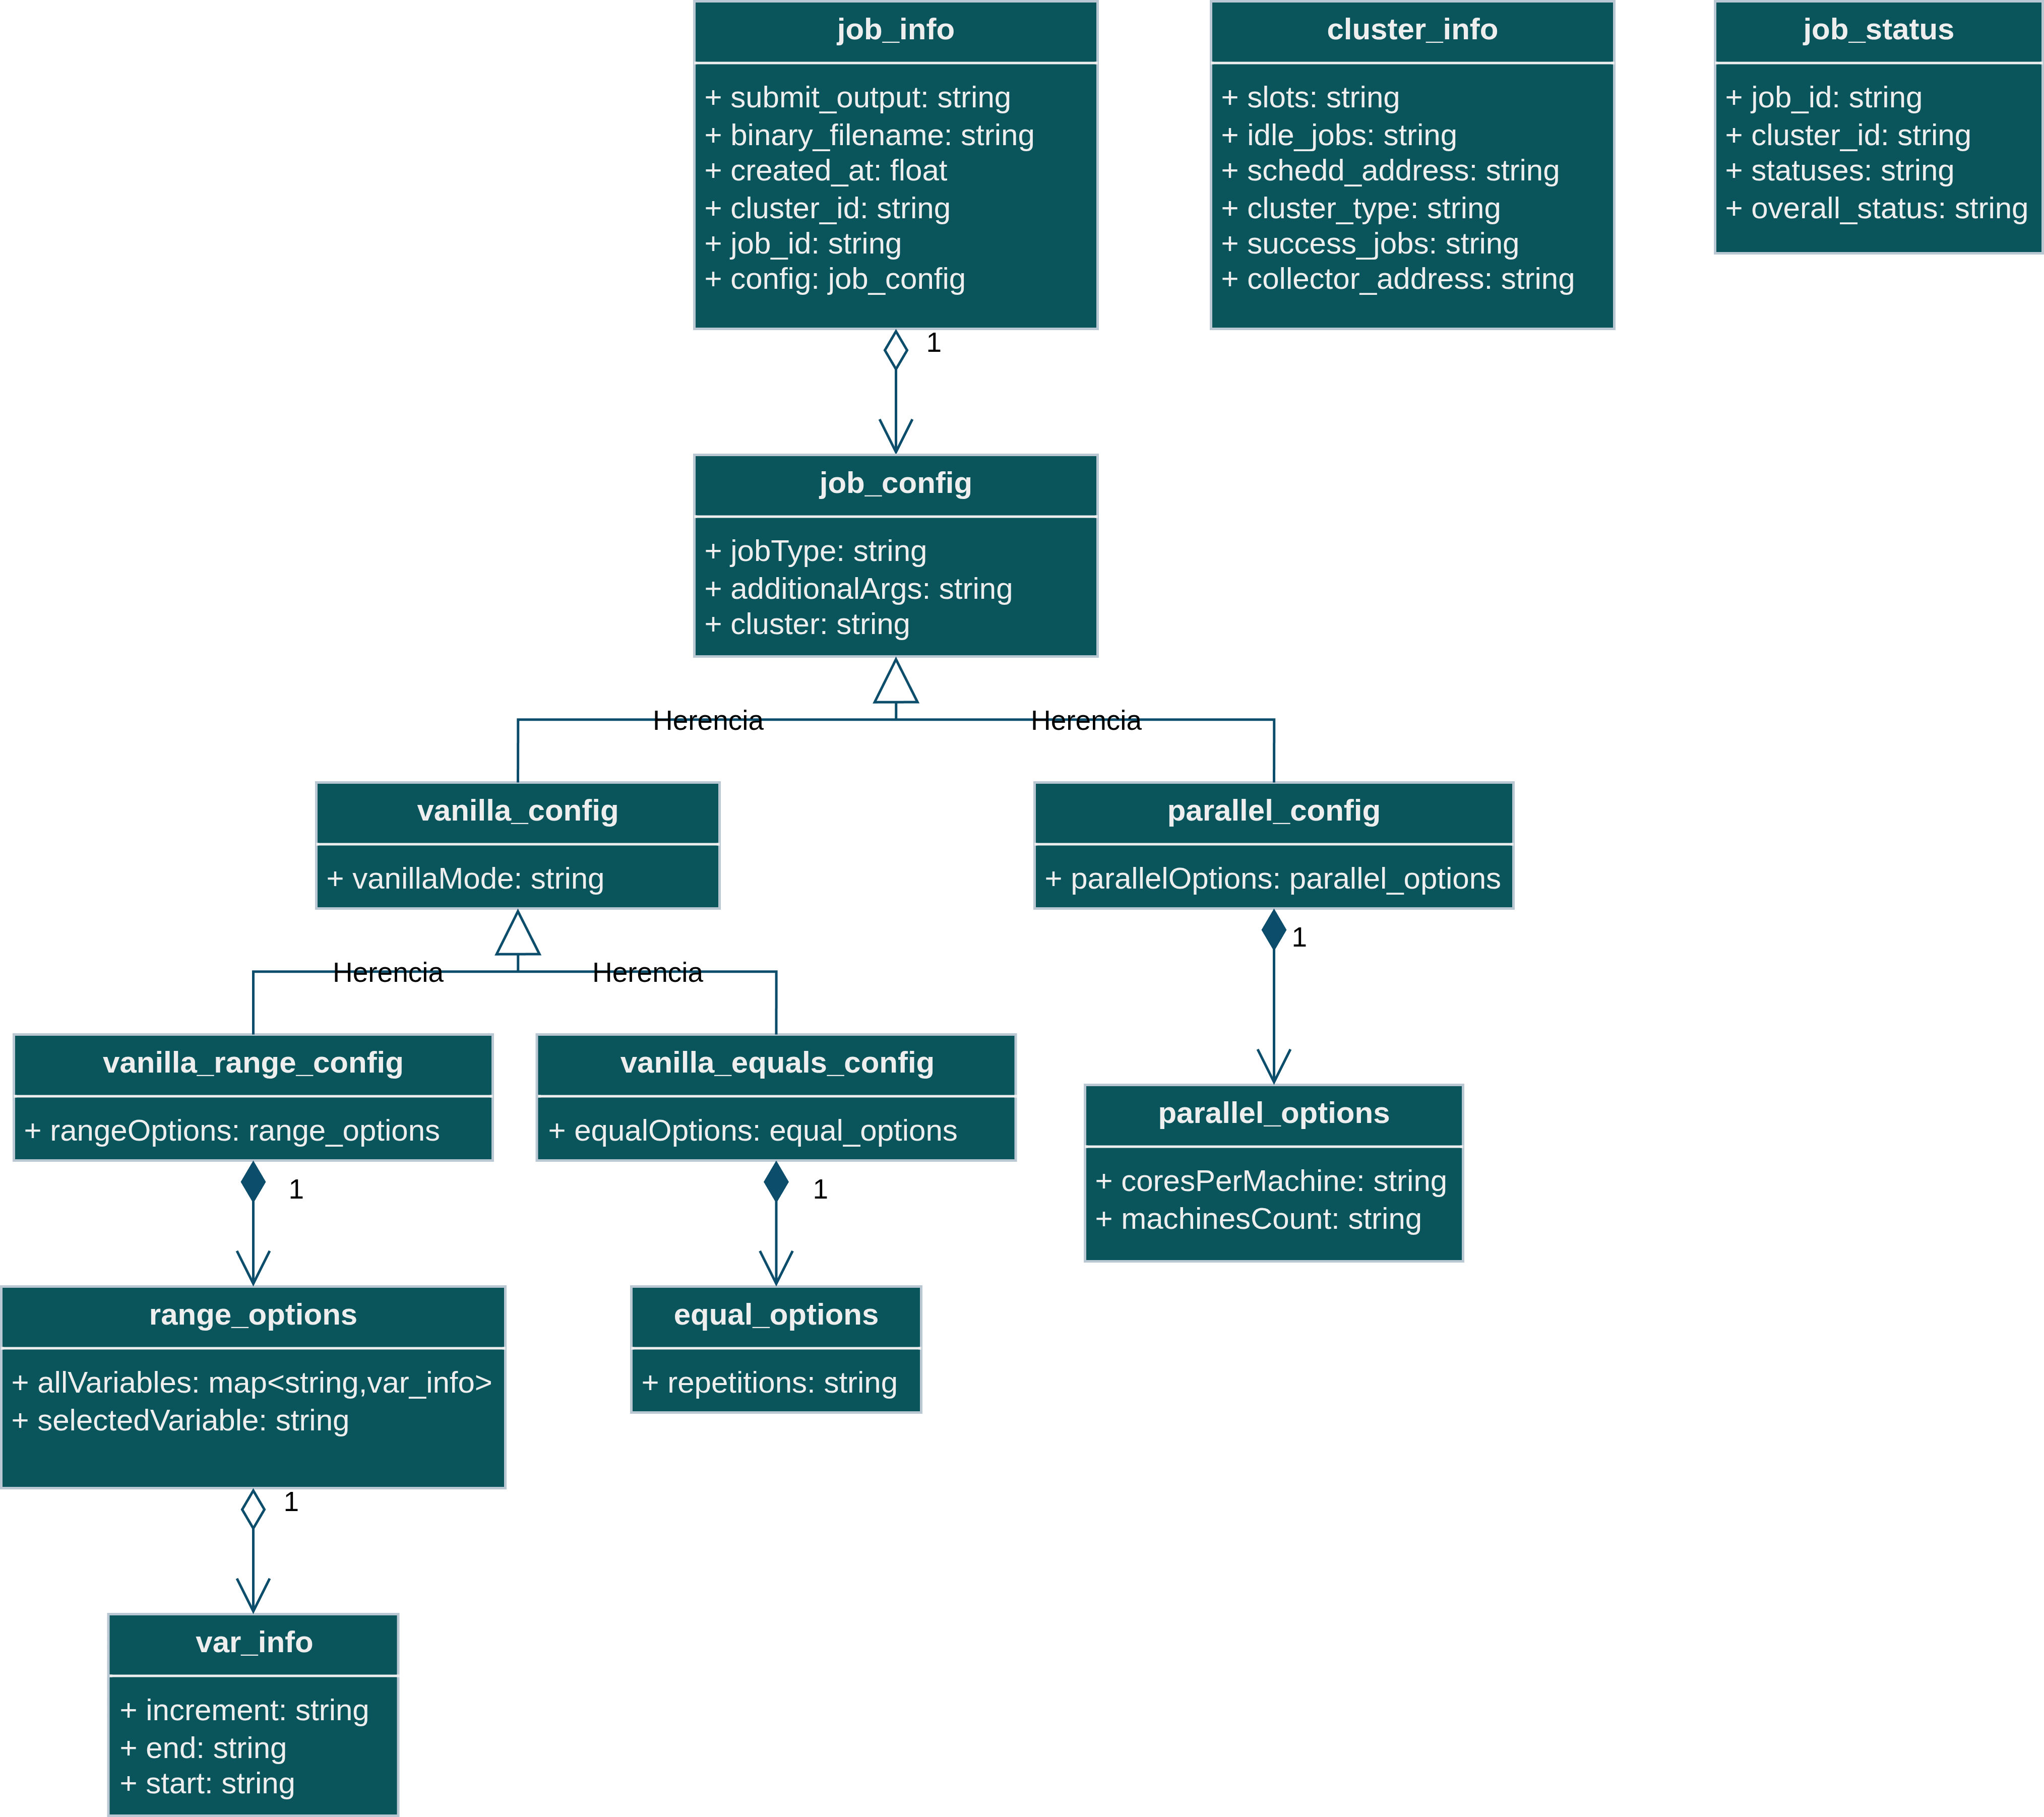
\includegraphics[scale=0.1]{tablas-images/UML/Diagramas HTCondor-Objetos.drawio.png}
	\caption{Diagrama de clases para el sistema}
    \label{fig:UMLClases}
\end{figure}

\section{Modelado de infraestructura con modelos personalizados}
Después de conocer como está compuesto el sistema de forma transversal con ArchiMate y en cuanto a software con C4 y \UML, se hace necesario un modelado más profundo de la infraestructura física y de red que compone la solución. Esto debido a que ArchiMate no da la profundidad necesaria para modelar esta clase de elementos, por lo que se opta por otras opciones con el fin de dar más profundidad al diseño y más claridad al lector sobre los elementos que componen la solución.

A pesar de esto, el equipo del proyecto no halló ningún lenguaje de modelado ni sistema formal que se armonizara con la clase de modelado de infraestructura que se pretende realizar. Por lo que se opta por usar una herramienta de modelado llamada draw.io y figuras genéricas con información complementaria que permiten tener una idea general de la infraestructura que subyace la solución.

\subsection{Modelo de infraestructura física}
\noindent
En la Figura \ref{fig:Fisica} se muestran los componentes de hardware principales que componen la solución. A su vez, se presentan las conexiones eléctricas que tiene cada elemento. Esto con el fin de mostrar la forma en que están conectados a la red eléctrica los componentes, ya que su conexión no es trivial y se hace necesaria documentación especializada que muestre este tipo de elementos.

\begin{figure}[H]
	\centering
	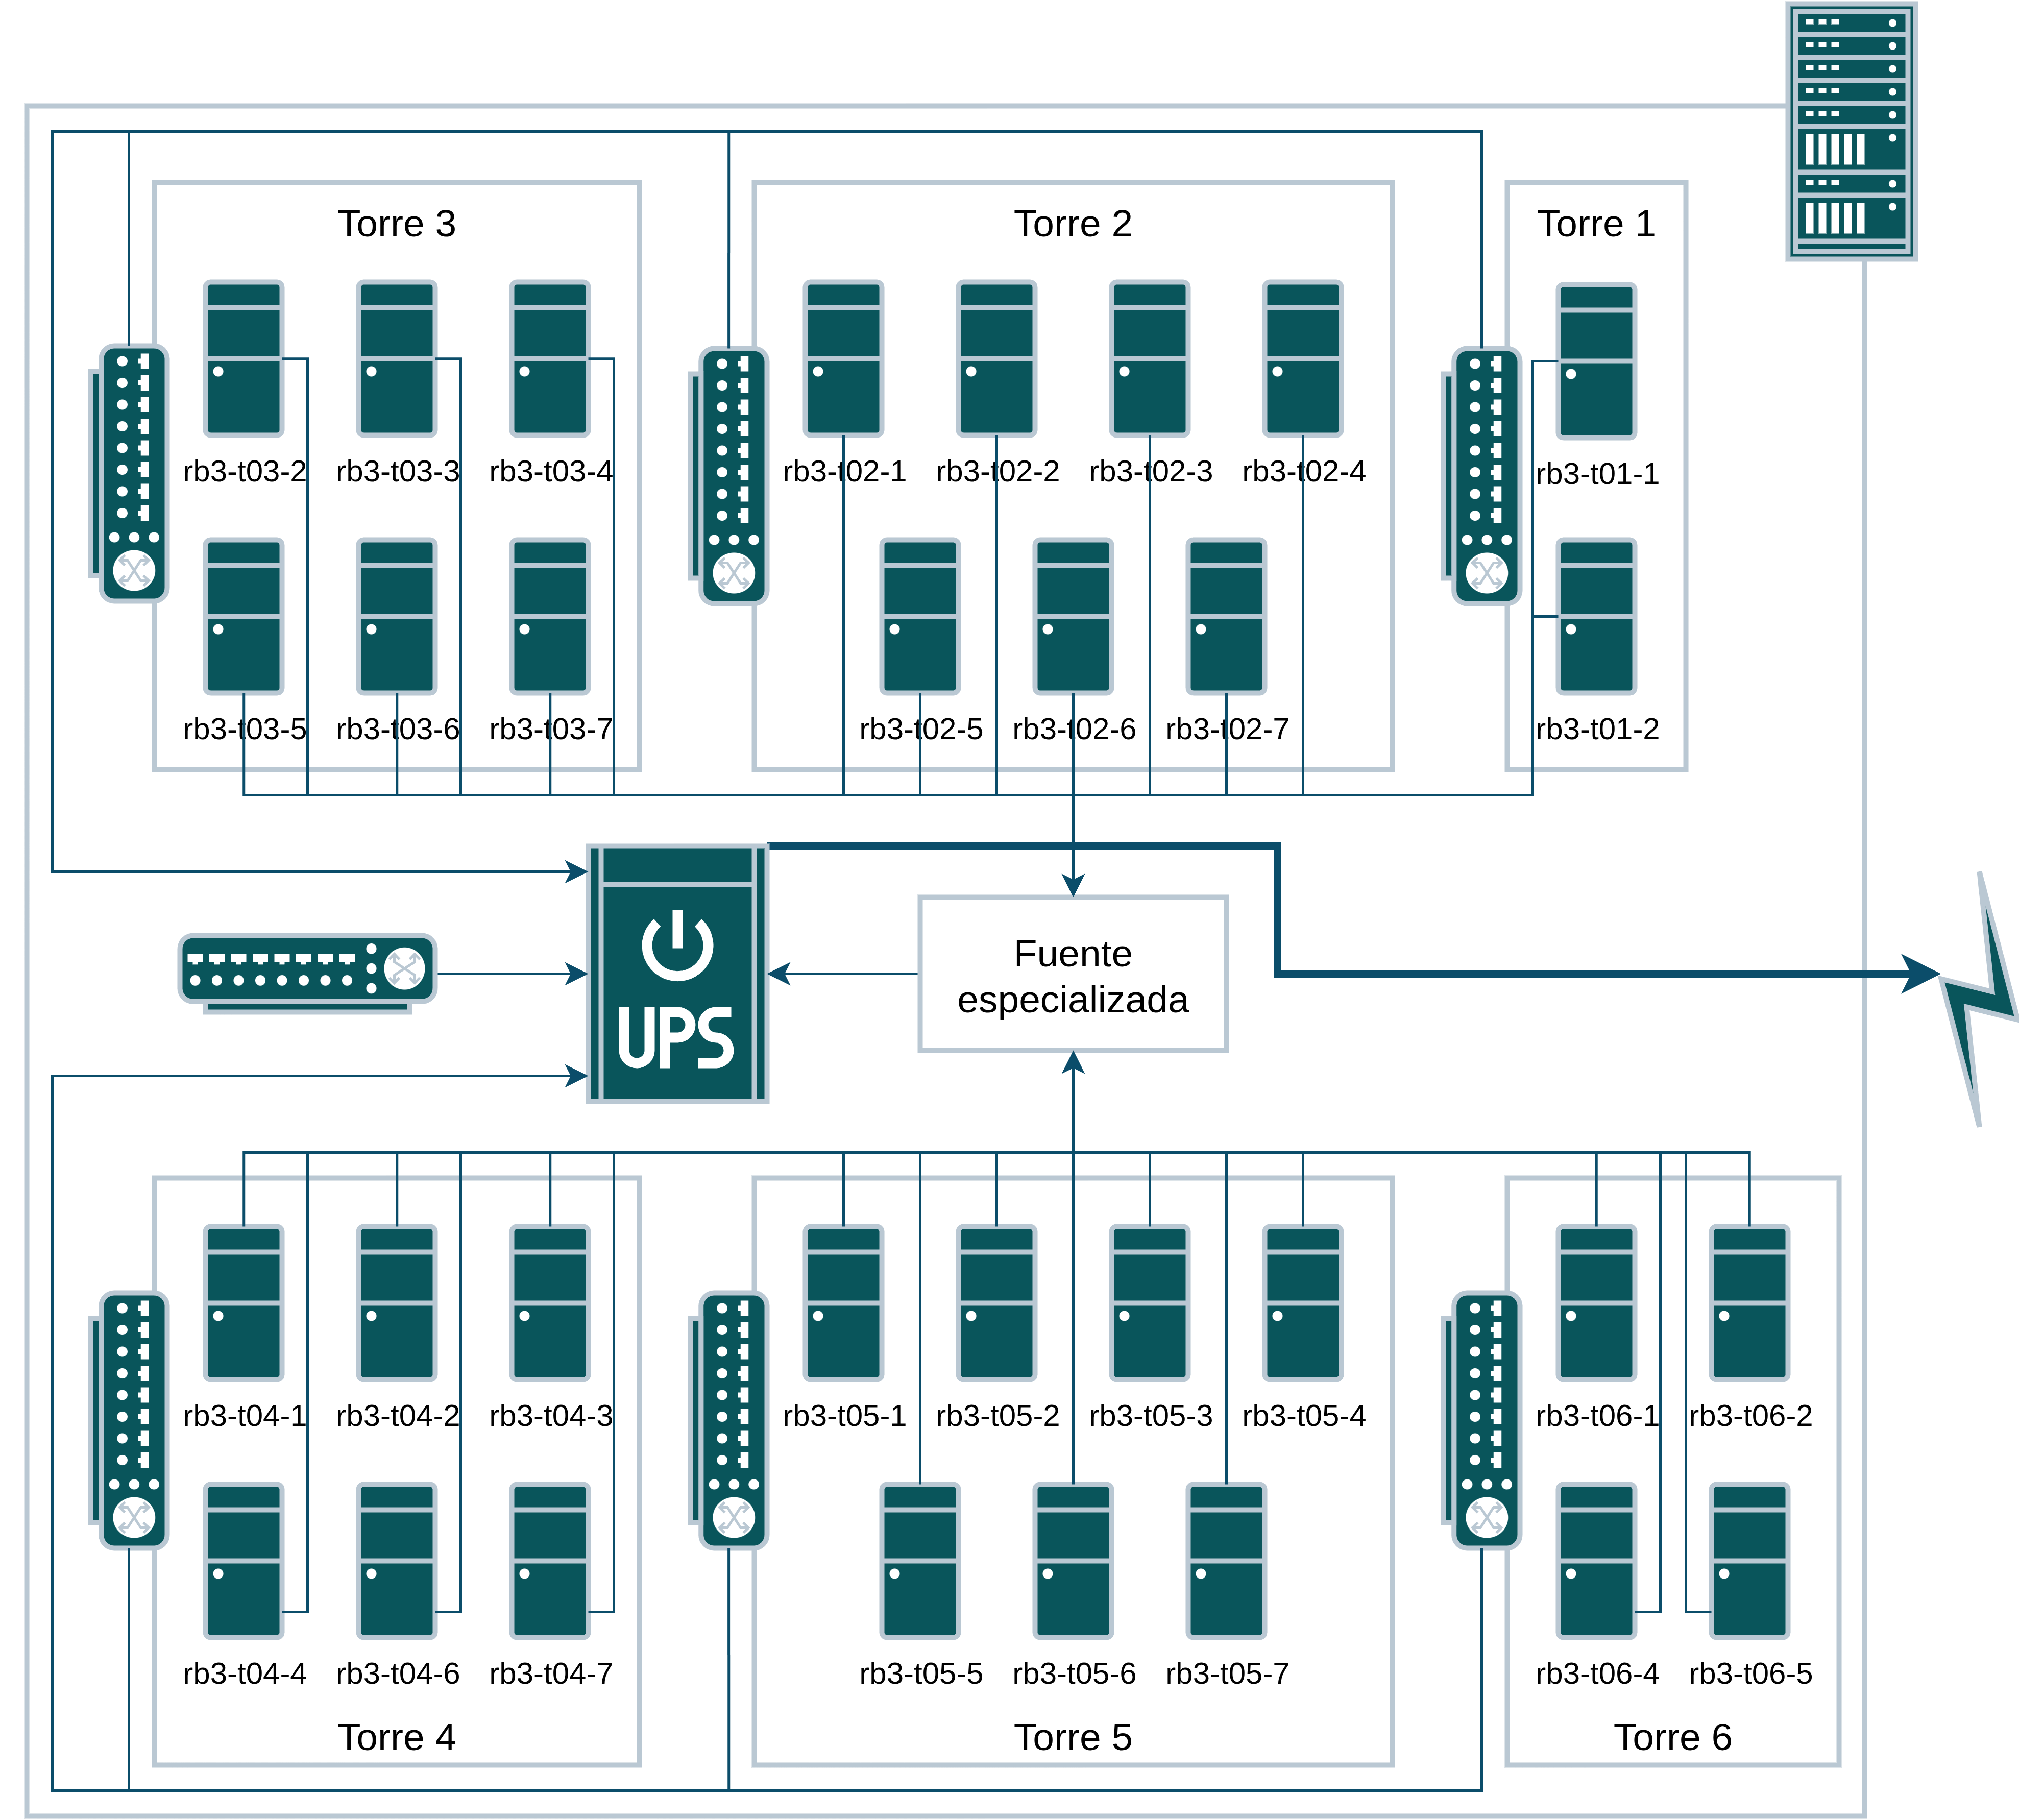
\includegraphics[scale=0.1]{tablas-images/personalizado/Diagramas HTCondor-Fisica.drawio.png}
	\caption{Modelo de infraestructura física}
    \label{fig:Fisica}
\end{figure}

\subsection{Modelo de enlace de datos}
\noindent
En la Figura \ref{fig:Enlace} se muestran las conexiones de red que tiene cada elemento. Esto con el fin de mostrar la forma en que están conectados los componentes a la red y a Internet, ya que su conexión no es trivial y se hace necesaria documentación especializada que muestre estás conexiones.

\begin{figure}[H]
	\centering
	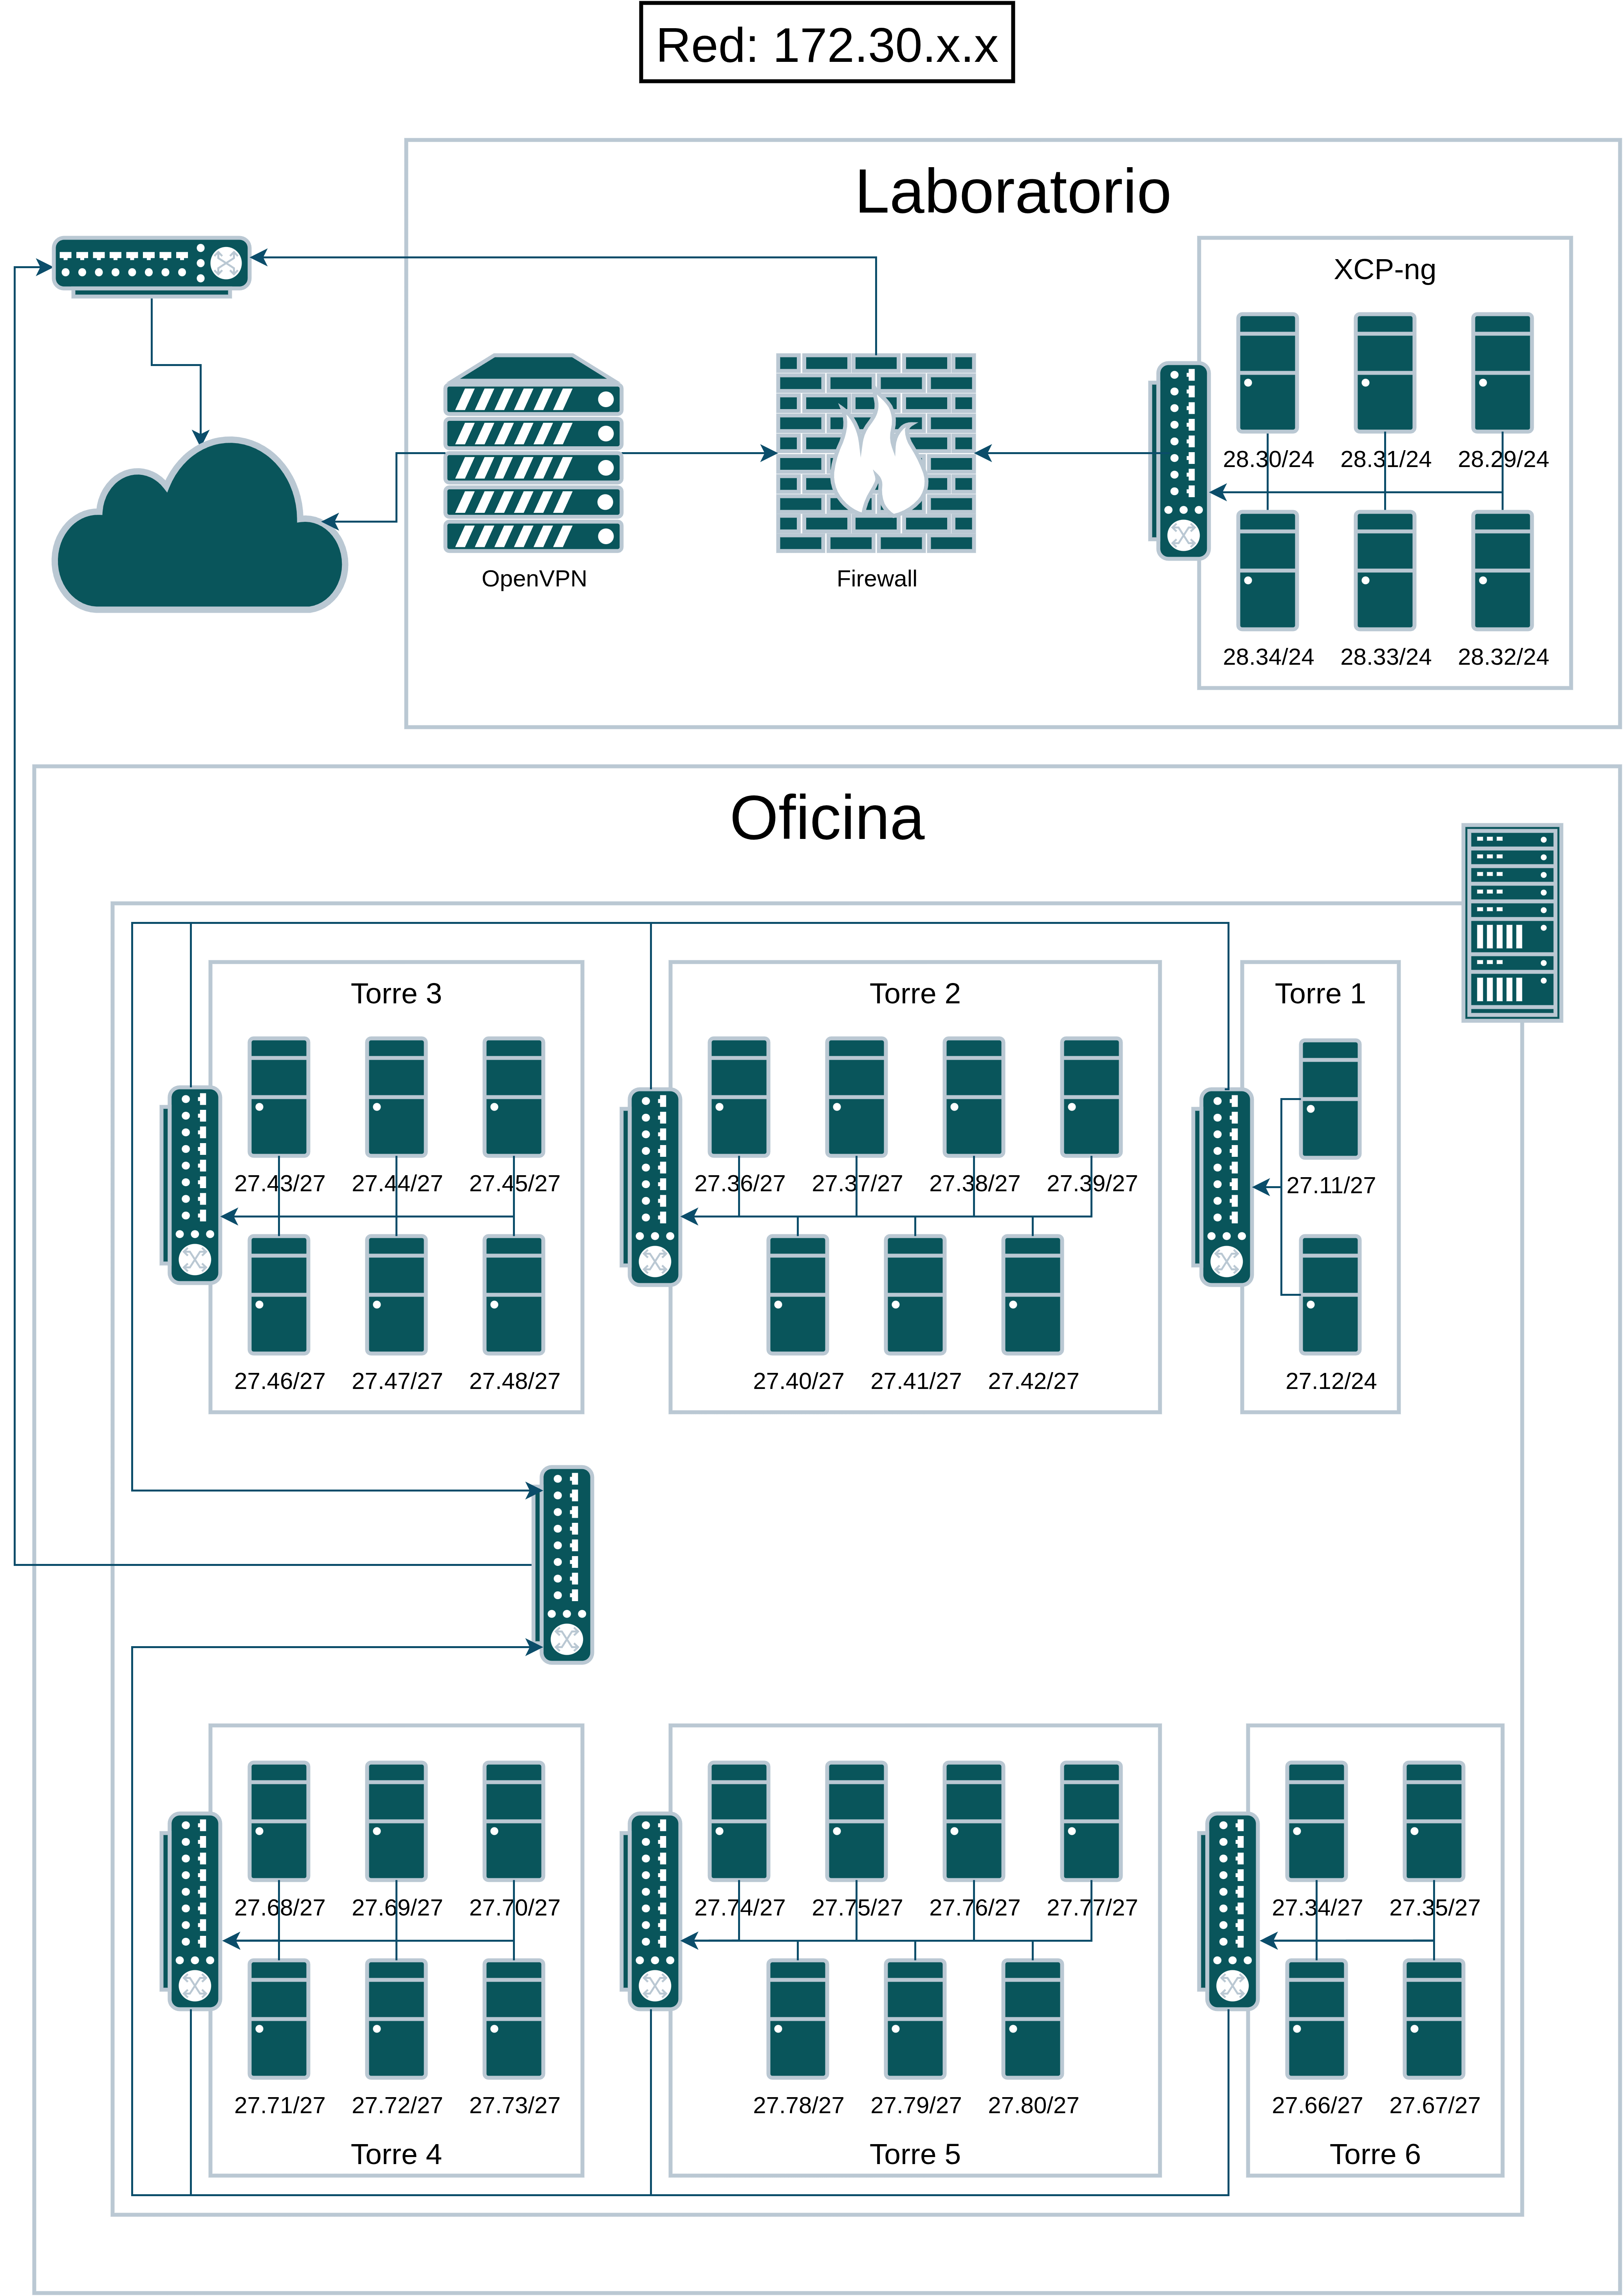
\includegraphics[scale=0.1]{tablas-images/personalizado/Diagramas HTCondor-Enlace.drawio.png}
	\caption{Modelo de enlace de datos}
    \label{fig:Enlace}
\end{figure}

\subsection{Modelo de roles}
\noindent
Después de conocer como están conectados los elementos de infraestructura a nivel eléctrico y de red, se hace necesario plasmar la forma en que están conectados los elementos de forma lógica, que es la forma en que se comunican los elementos en el diseño de la solución. Además, se hace necesario mostrar los roles de HTCondor que ocupa cada elemento en su clúster. En la Figura \ref{fig:Roles} se plasman estos aspectos.

\begin{figure}[H]
	\centering
	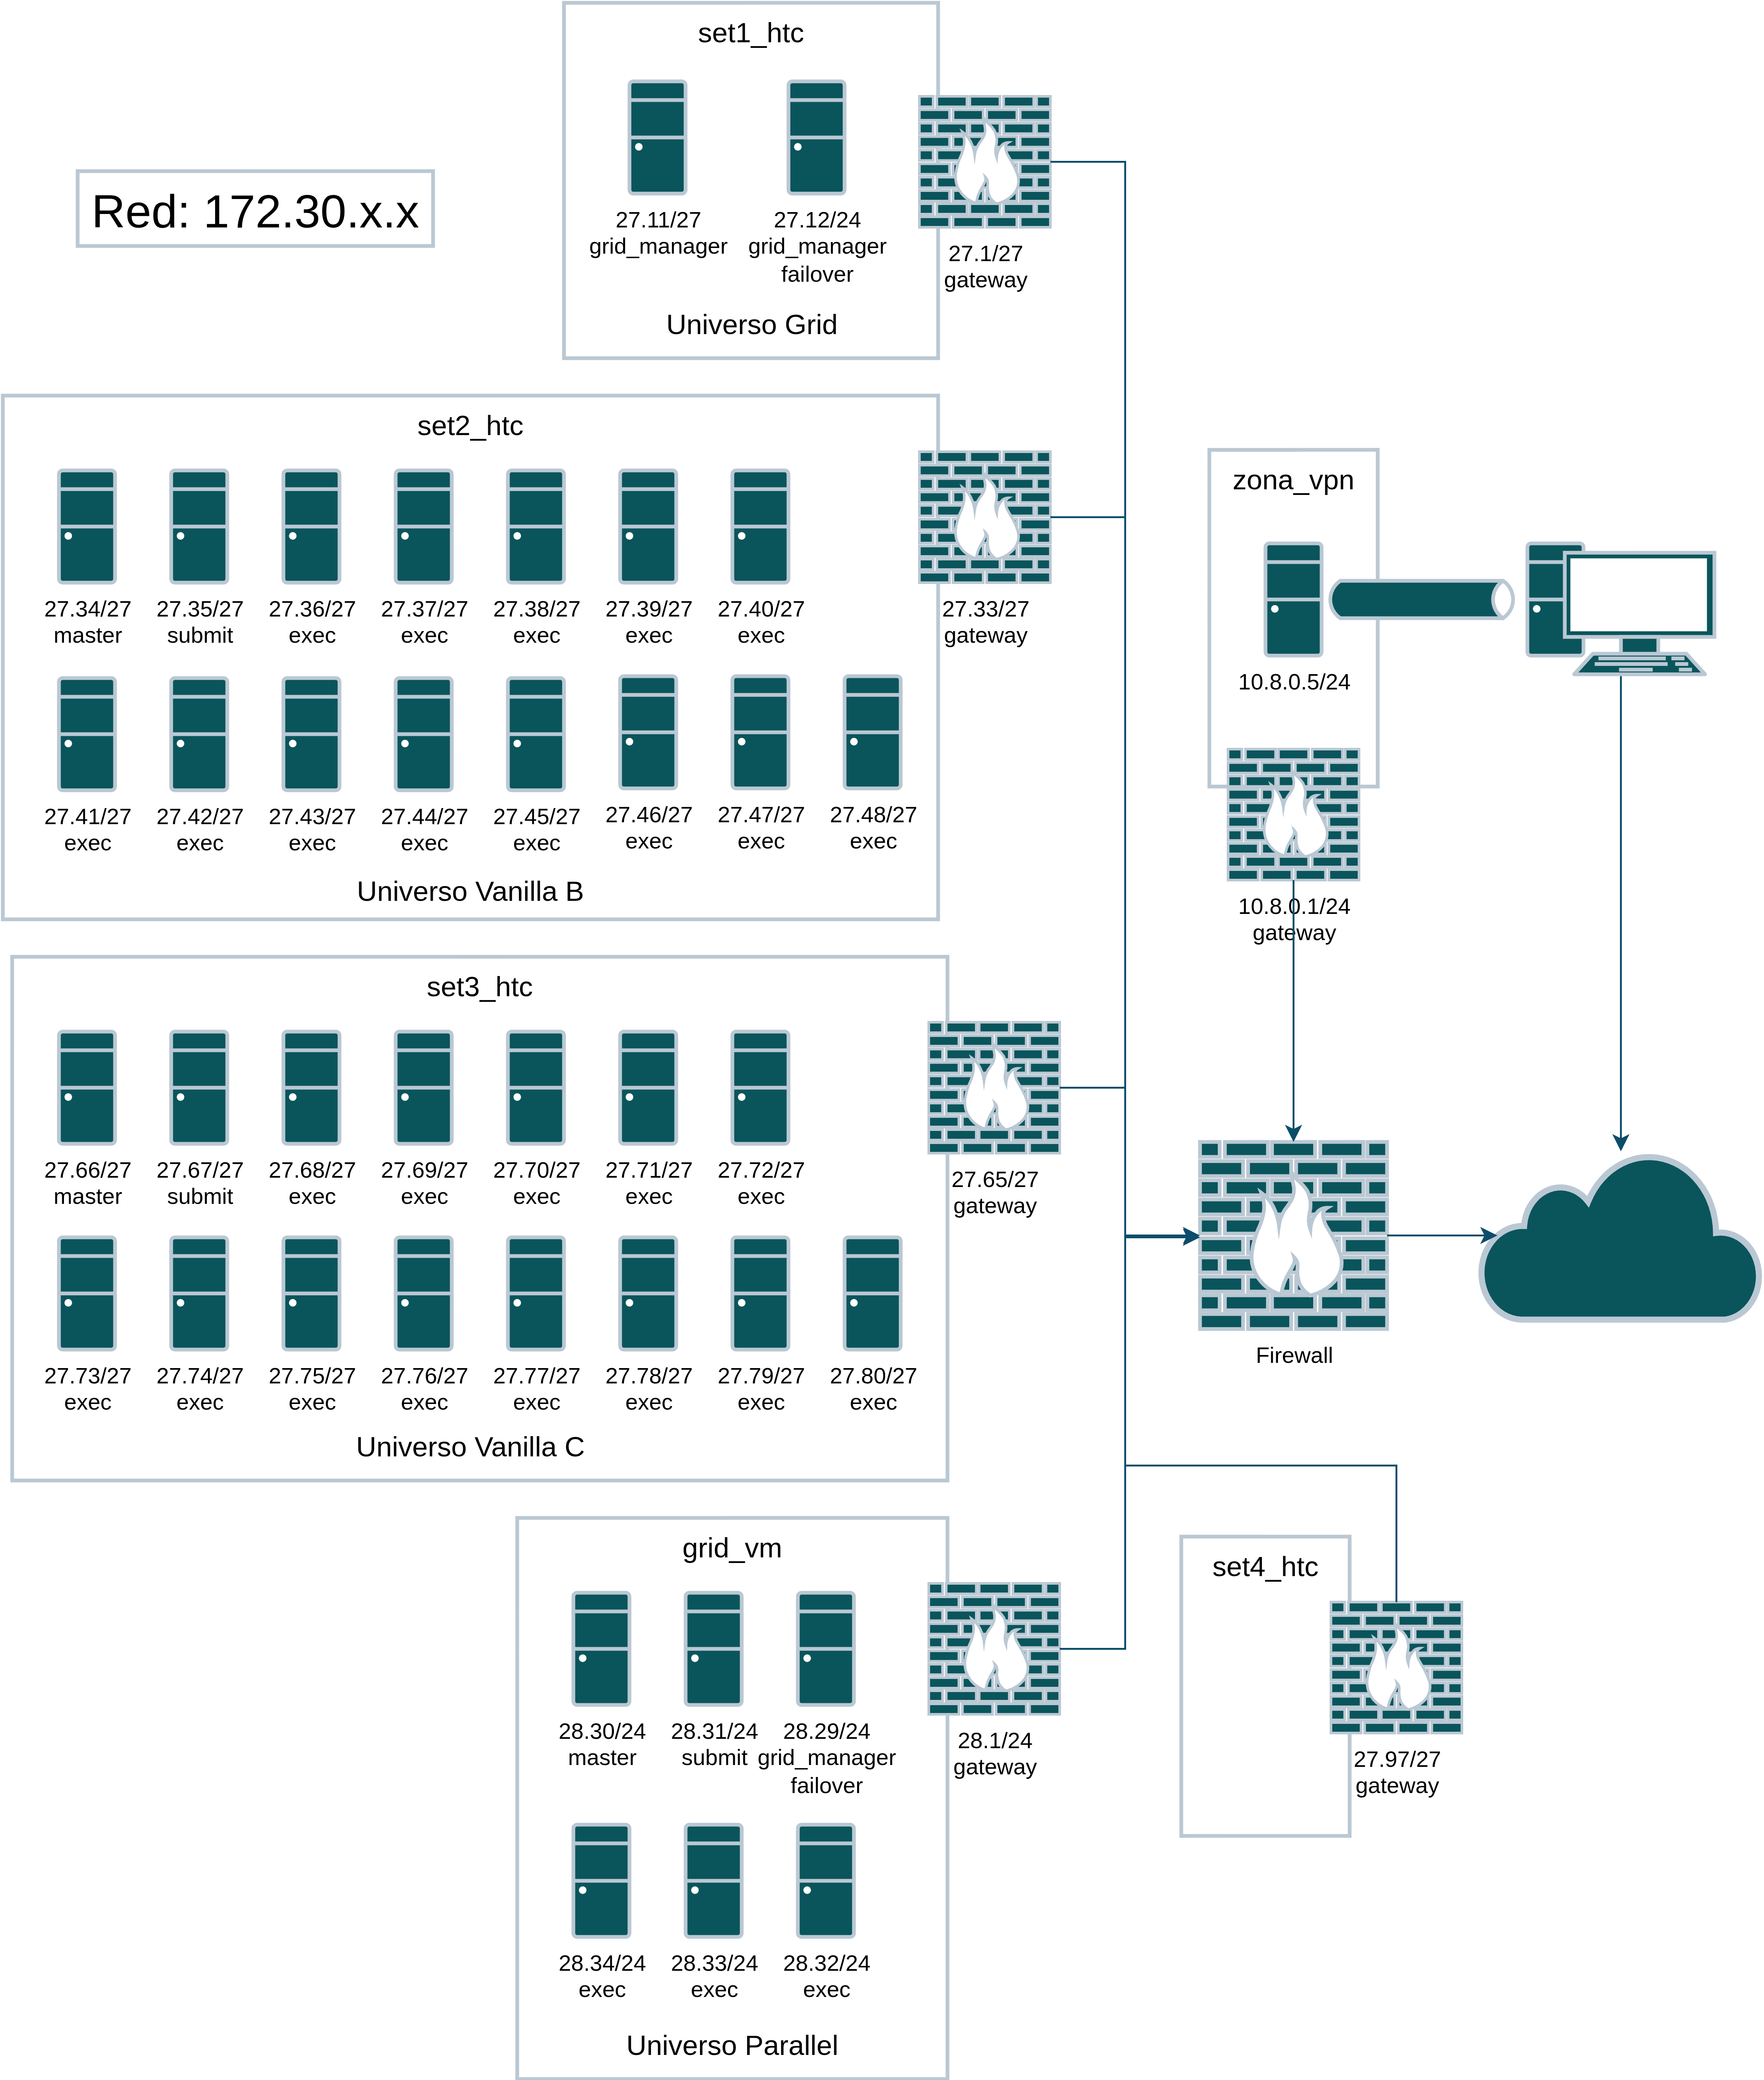
\includegraphics[scale=0.088]{tablas-images/personalizado/Diagramas HTCondor-Roles.drawio.png}
	\caption{Modelo de roles}
    \label{fig:Roles}
\end{figure}